% Includable chapter. Requires amsmath, amssymb, graphicx, caption,
% tikz, hyperref, and float.
\chapter{Measuring the world with geometry}
\label{chap:geometry}
\begin{center}\large Geometry as a way of reasoning\end{center}
\begin{center}
\begin{minipage}[t]{0.47\textwidth}
\centering\vspace{0pt}
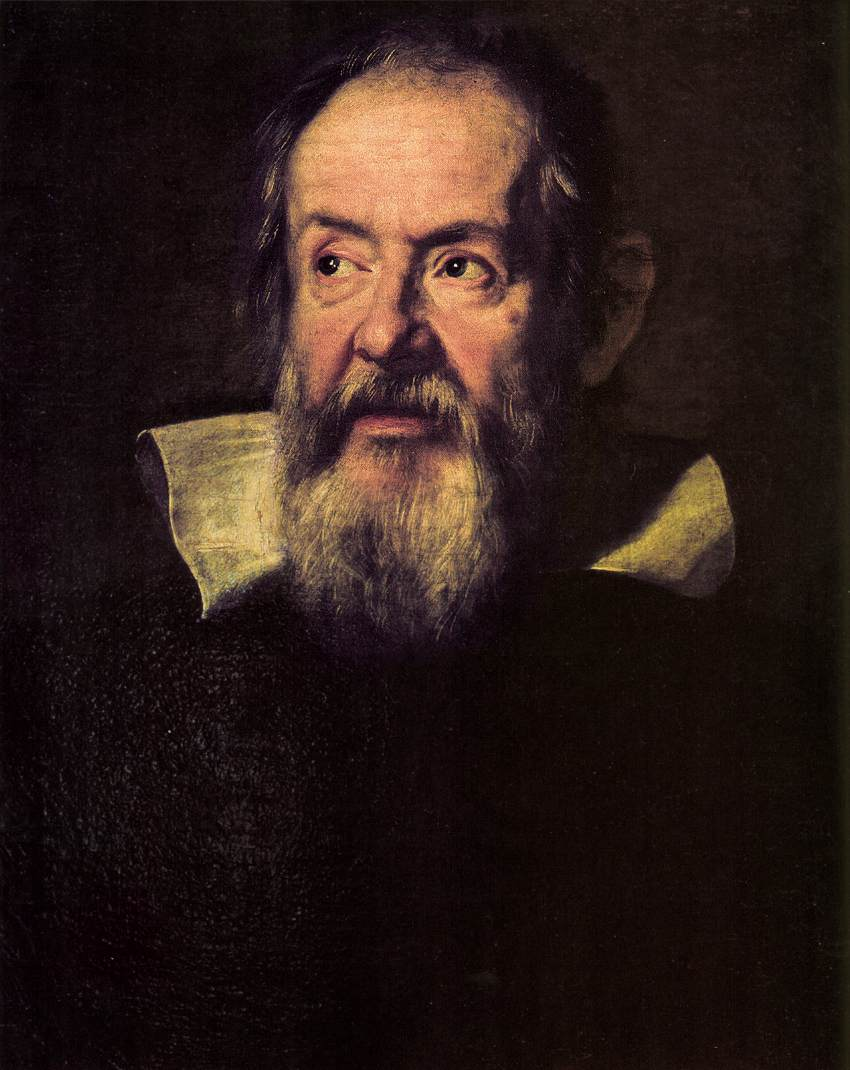
\includegraphics[height=1.25in]{images/galileo.jpg}
\captionof*{figure}{\small ``It is written in the language of mathematics, and its characters are triangles, circles, and other geometric figures''\\
---Galileo Galilei, \href{https://old.maa.org/press/periodicals/convergence/quotations-in-context-galileo-2}{\emph{The Assayer}} (1623), excerpt; translated by Stillman Drake.}
{\scriptsize Portrait by Justus Sustermans, 1636. Public domain.}
\end{minipage}\hfill
\begin{minipage}[t]{0.47\textwidth}
\centering\vspace{0pt}
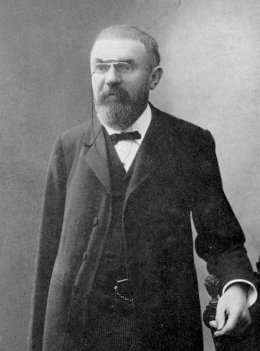
\includegraphics[height=1.25in]{images/poincare.jpg}
\captionof*{figure}{\small ``it is by logic one demonstrates, by intuition one invents.''\\
---Henri Poincar\'e, \href{https://www.gutenberg.org/files/39713/39713-h/39713-h.htm}{\emph{Science and Method}}, Book II, Chapter II; excerpt, translated by G.~B.~Halsted.}
{\scriptsize Frontispiece of \emph{Last Thoughts}, 1913. Public-domain image (Wikimedia Commons).}
\end{minipage}
\end{center}

How can we measure a building without climbing it? Locate ourselves from
distances to landmarks? Find a shortest route that has to touch a boundary?
Choose a shape that uses a fixed amount of material efficiently?
These questions ask us to do more than remember a formula. We must decide
what to represent, what to measure, and why the resulting construction works.

In the preceding chapters, a proof guided the construction of an algorithm.
Geometry lets us follow the same approach with diagrams. A figure suggests
relationships; a proof explains which of them must hold. We will use
similar triangles, lengths, areas, and volumes that are already familiar,
and turn them into tools for solving practical problems.

\section{From a place to a geometric model}
\label{sec:geo-model}
A building has windows, ledges, and an irregular roof. For a shadow
measurement, we may represent it by a vertical segment of unknown length.
We represent level ground by a straight line and sunlight by parallel
rays. These choices form a \emph{model}: we retain the features relevant
to the question and set others aside.

A conclusion can be correct within a model and still give a poor answer
about the place being measured. Perhaps the ground slopes, the building
leans, or we measure the shadow of the wrong part of the roof. We therefore
keep two questions separate: does the reasoning follow from the assumptions,
and are those assumptions suitable here?

\begin{figure}[htbp]\centering
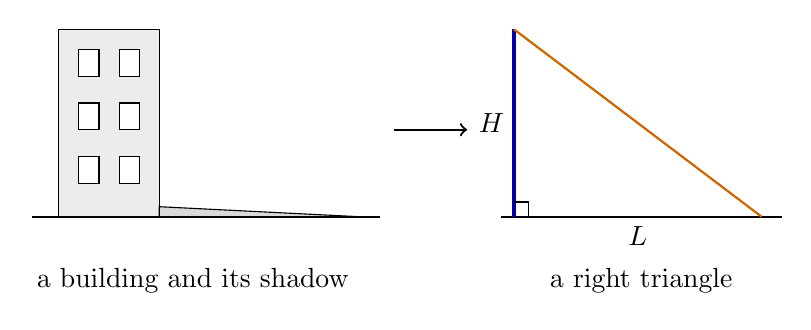
\begin{tikzpicture}[scale=.85]
\draw[fill=gray!15] (0,0) rectangle (1.5,2.8);
\foreach \x in {.3,.9}{\foreach \y in {.5,1.3,2.1}{\draw[fill=white] (\x,\y) rectangle +(0.3,.4);}}
\draw[thick] (-.4,0)--(4.8,0);\draw[fill=gray!30] (1.5,0)--(4.5,0)--(1.5,.15)--cycle;
\node at (2,-.95) {a building and its shadow};
\draw[->,thick] (5,1.3)--(6.1,1.3);
\draw[thick] (6.6,0)--(10.8,0);\draw[very thick,blue!65!black] (6.8,0)--(6.8,2.8);
\draw[orange!80!black,thick] (6.8,2.8)--(10.5,0);
\draw (6.8,.22)--(7.02,.22)--(7.02,0);
\node[left] at (6.8,1.4) {$H$};\node[below] at (8.65,0) {$L$};
\node at (8.7,-.95) {a right triangle};
\end{tikzpicture}
\caption{A model makes selected relationships explicit. The right angle is an assumption to check, not a consequence of the drawing.}
\end{figure}

Throughout this chapter we use plane Euclidean geometry for local maps,
and straight-line distance unless another notion of distance is specified.
Diagrams explain the construction; their drawn sizes are not measurements.

\section{Measuring what we cannot reach}
\label{sec:geo-measure}
\subsection{A building and a stick}
\paragraph{The problem.}
Determine the height $H$ of a vertical building from a stick of known
height $h>0$ and simultaneous shadow lengths $s>0$ (stick) and $L>0$
(building). Assume level ground, vertical objects, and parallel sunlight.

Place a vertical stick
of known height $h$ on the same level ground, and measure its shadow $s$
and the building's shadow $L$ at the same time. Assume the tips of both
shadows can be identified and the Sun is above the horizon, so $s>0$.

The two right triangles have the same angle with the sunlight, whose rays
we treat as parallel. They are similar, and hence
\[
\frac{H}{L}=\frac{h}{s},\qquad H=\frac{hL}{s}.
\]
The inaccessible length has been replaced by three accessible ones.

\begin{figure}[htbp]\centering
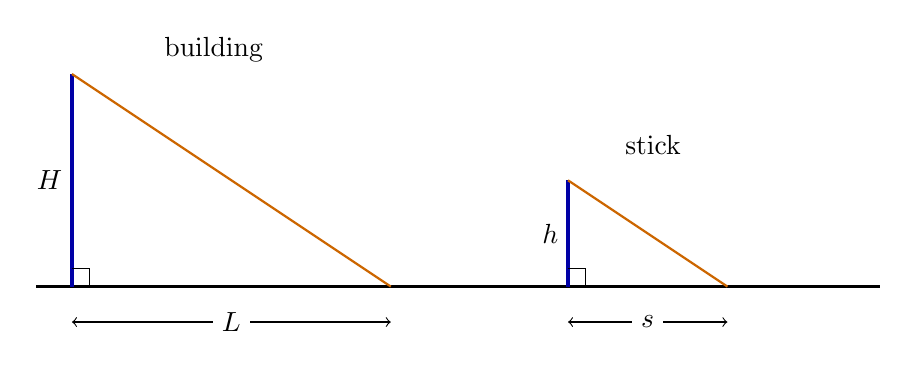
\begin{tikzpicture}[scale=.9]
\draw[thick] (-.5,0)--(11.4,0);
\draw[very thick,blue!65!black] (0,0)--(0,3);
\draw[orange!80!black,thick] (0,3)--(4.5,0);
\draw[very thick,blue!65!black] (7,0)--(7,1.5);
\draw[orange!80!black,thick] (7,1.5)--(9.25,0);
\draw (0,.25)--(.25,.25)--(.25,0);\draw (7,.25)--(7.25,.25)--(7.25,0);
\node[left] at (0,1.5) {$H$};\node[left] at (7,.75) {$h$};
\draw[<->] (0,-.5)--node[fill=white]{$L$}(4.5,-.5);
\draw[<->] (7,-.5)--node[fill=white]{$s$}(9.25,-.5);
\node at (2,3.35) {building};\node at (8.2,2) {stick};
\end{tikzpicture}
\caption{Equal sunlight angles and vertical objects give similar triangles.}
\label{fig:geo-shadows}
\end{figure}

\paragraph{A measurement procedure.}
First check verticality and the ground. Measure $h$, then measure $s$ and
$L$ as nearly simultaneously as possible. Calculate $hL/s$ and record the
units and the conditions under which the measurement was made.
For $h=1.5$ metres, $s=2$ metres, and $L=18$ metres, the estimate is
$H=13.5$ metres. The numerical answer alone does not tell us how accurate
it is.

\subsection{How much should we trust the answer?}
Suppose $h=1.5$ metres is treated as exact, but the shadow measurements
lie in the intervals
\[
17.8\leq L\leq18.2,\qquad1.9\leq s\leq2.1.
\]
\paragraph{The problem.}
Under the same shadow model, find lower and upper bounds for $H$ that
contain every value consistent with these measurement intervals. All
lengths in the displayed intervals are in metres.

Increasing $L$ increases $H$, while increasing the positive denominator
$s$ decreases it. Consequently,
\[
\frac{1.5(17.8)}{2.1}\leq H\leq\frac{1.5(18.2)}{1.9},
\qquad 12.71\ldots\leq H\leq14.36\ldots.
\]
A conservative rounded report is $12.7\leq H\leq14.4$ metres.
This interval accounts for the stated measurement uncertainty within the
model; it does not account for a leaning stick or sloping ground.

\begin{figure}[htbp]\centering
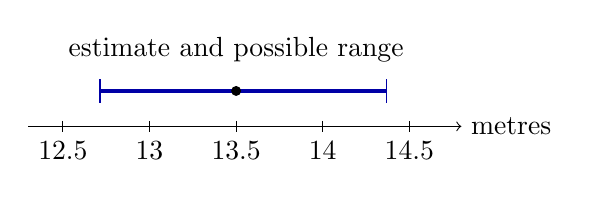
\begin{tikzpicture}[x=2.2cm,y=1cm]
\draw[->] (12.3,0)--(14.8,0) node[right]{metres};
\foreach \x in {12.5,13,13.5,14,14.5}{\draw (\x,.07)--(\x,-.07) node[below]{$\x$};}
\draw[very thick,blue!65!black] (12.714,.45)--(14.368,.45);
\draw[blue!65!black] (12.714,.3)--(12.714,.6) (14.368,.3)--(14.368,.6);
\fill (13.5,.45) circle (1.8pt);\node[above] at (13.5,.7) {estimate and possible range};
\end{tikzpicture}
\caption{An interval often communicates a measurement more honestly than extra decimal places.}
\end{figure}

If a shadow is very short, a small absolute error can be a large fraction
of its length. A longer shadow may help, but a low Sun can make its tip
harder to identify. A useful procedure must consider both the geometry
and the quality of the observations.

\subsection{Can a photograph replace a shadow?}
\label{sec:geo-camera}
A shadow turned an inaccessible height into a ratio of accessible lengths.
Could a smartphone photograph do the same job? A photograph also records
rays of light, but its geometry is different. Sunlight was modelled by
parallel rays; a camera is modelled by rays passing through a single point,
the \emph{camera centre}. Similar triangles will again do the work.

\paragraph{A dark room, a small hole, and a picture.}
The point-camera model has a physical counterpart: a dark box with a small
hole in one side and a screen opposite it. Light from the top of an object
passes through the hole and reaches the lower part of the screen; light
from the bottom reaches the upper part. The image is inverted. A darkened
room can do the same thing, which explains the name \emph{camera obscura},
Latin for ``dark room''. A pinhole camera uses this principle without a
lens. The image can be viewed on a screen; recording it permanently
requires a light-sensitive surface.

\begin{figure}[htbp]\centering
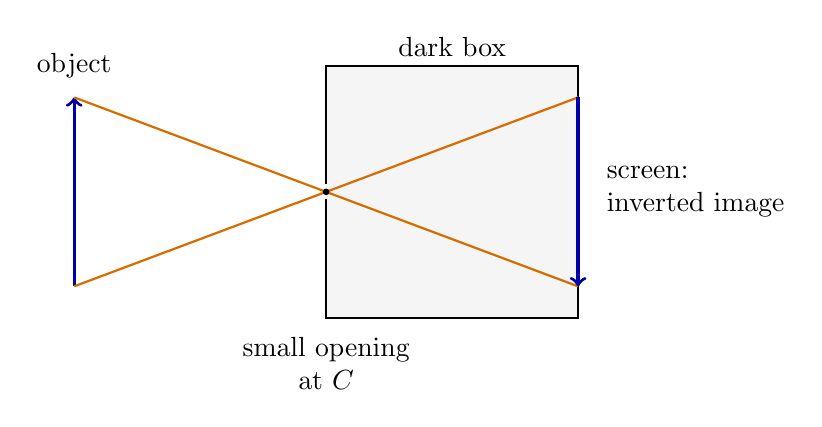
\begin{tikzpicture}[scale=.8]
\fill[gray!8] (0,-2) rectangle (4,2);
\draw[thick] (0,.12)--(0,2)--(4,2)--(4,-2)--(0,-2)--(0,-.12);
\draw[very thick,blue!65!black,->] (-4,-1.5)--(-4,1.5);
\draw[orange!85!black,thick] (-4,1.5)--(4,-1.5);
\draw[orange!85!black,thick] (-4,-1.5)--(4,1.5);
\draw[very thick,blue!65!black,->] (4,1.5)--(4,-1.5);
\fill (0,0) circle(1.5pt);
\node[above] at (-4,1.65) {object};
\node[above] at (2,2) {dark box};
\node[below,align=center] at (0,-2.15) {small opening\\at $C$};
\node[right,align=left] at (4.3,0) {screen:\\inverted image};
\end{tikzpicture}
\caption{The camera obscura principle. Rays cross at the small opening;
the screen is behind it, on the opposite side from the object. The arrows
represent the object and its inverted image, not the direction of light. The ideal pinhole cannot physically exist. Modern cameras are approximations of the ideal model.}
\label{fig:geo-pinhole}
\end{figure}

Pinhole-image effects were known in antiquity. In the eleventh century,
Ibn al-Haytham (Alhazen, c.~965--c.~1040) investigated light and vision
through mathematical reasoning and experiments, including dark-room
arrangements. His work helped establish how straight-travelling light
produces images and how vision depends on light entering the eye. \footnote{For Ibn al-Haytham's experimental approach, see
\href{https://www.unesco.org/en/articles/ibn-al-haythams-scientific-method}{UNESCO, ``Ibn al-Haytham's scientific method''}, and
\href{https://www.ibnalhaytham.com/discover/who-was-ibn-al-haytham/}{``Who was Ibn al-Haytham?''}.
The \href{https://www.cameramuseum.ch/en/discover/permanent-exhibition/the-origins-of-photography/the-camera-obscura/}{Swiss Camera Museum}
discusses the camera obscura's ancient antecedents and later use as a drawing instrument.}

\begin{figure}[htbp]\centering
\begin{minipage}[t]{.46\textwidth}\centering\vspace{0pt}
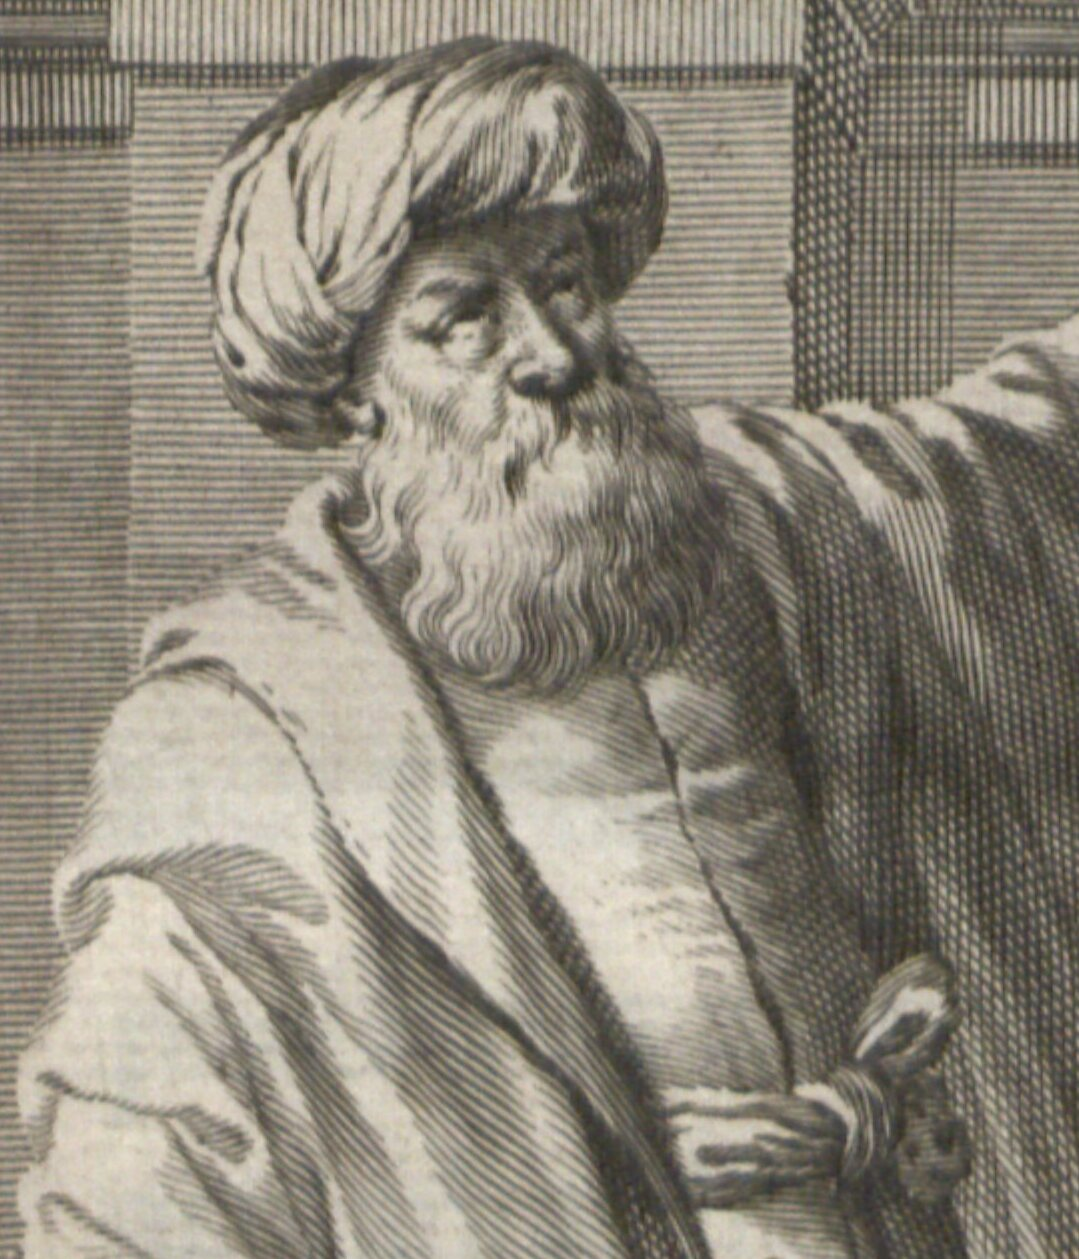
\includegraphics[height=1.65in]{images/ibn-al-haytham.jpg}\par\smallskip
\small Ibn al-Haytham, as imagined in the frontispiece of Hevelius's
\emph{Selenographia} (1647). A later representation, not a contemporary
likeness. \href{https://commons.wikimedia.org/wiki/File:Alhazen_(122459248).jpg}{Polona / Wikimedia Commons; public domain.}
\end{minipage}\hfill
\begin{minipage}[t]{.46\textwidth}\centering\vspace{0pt}
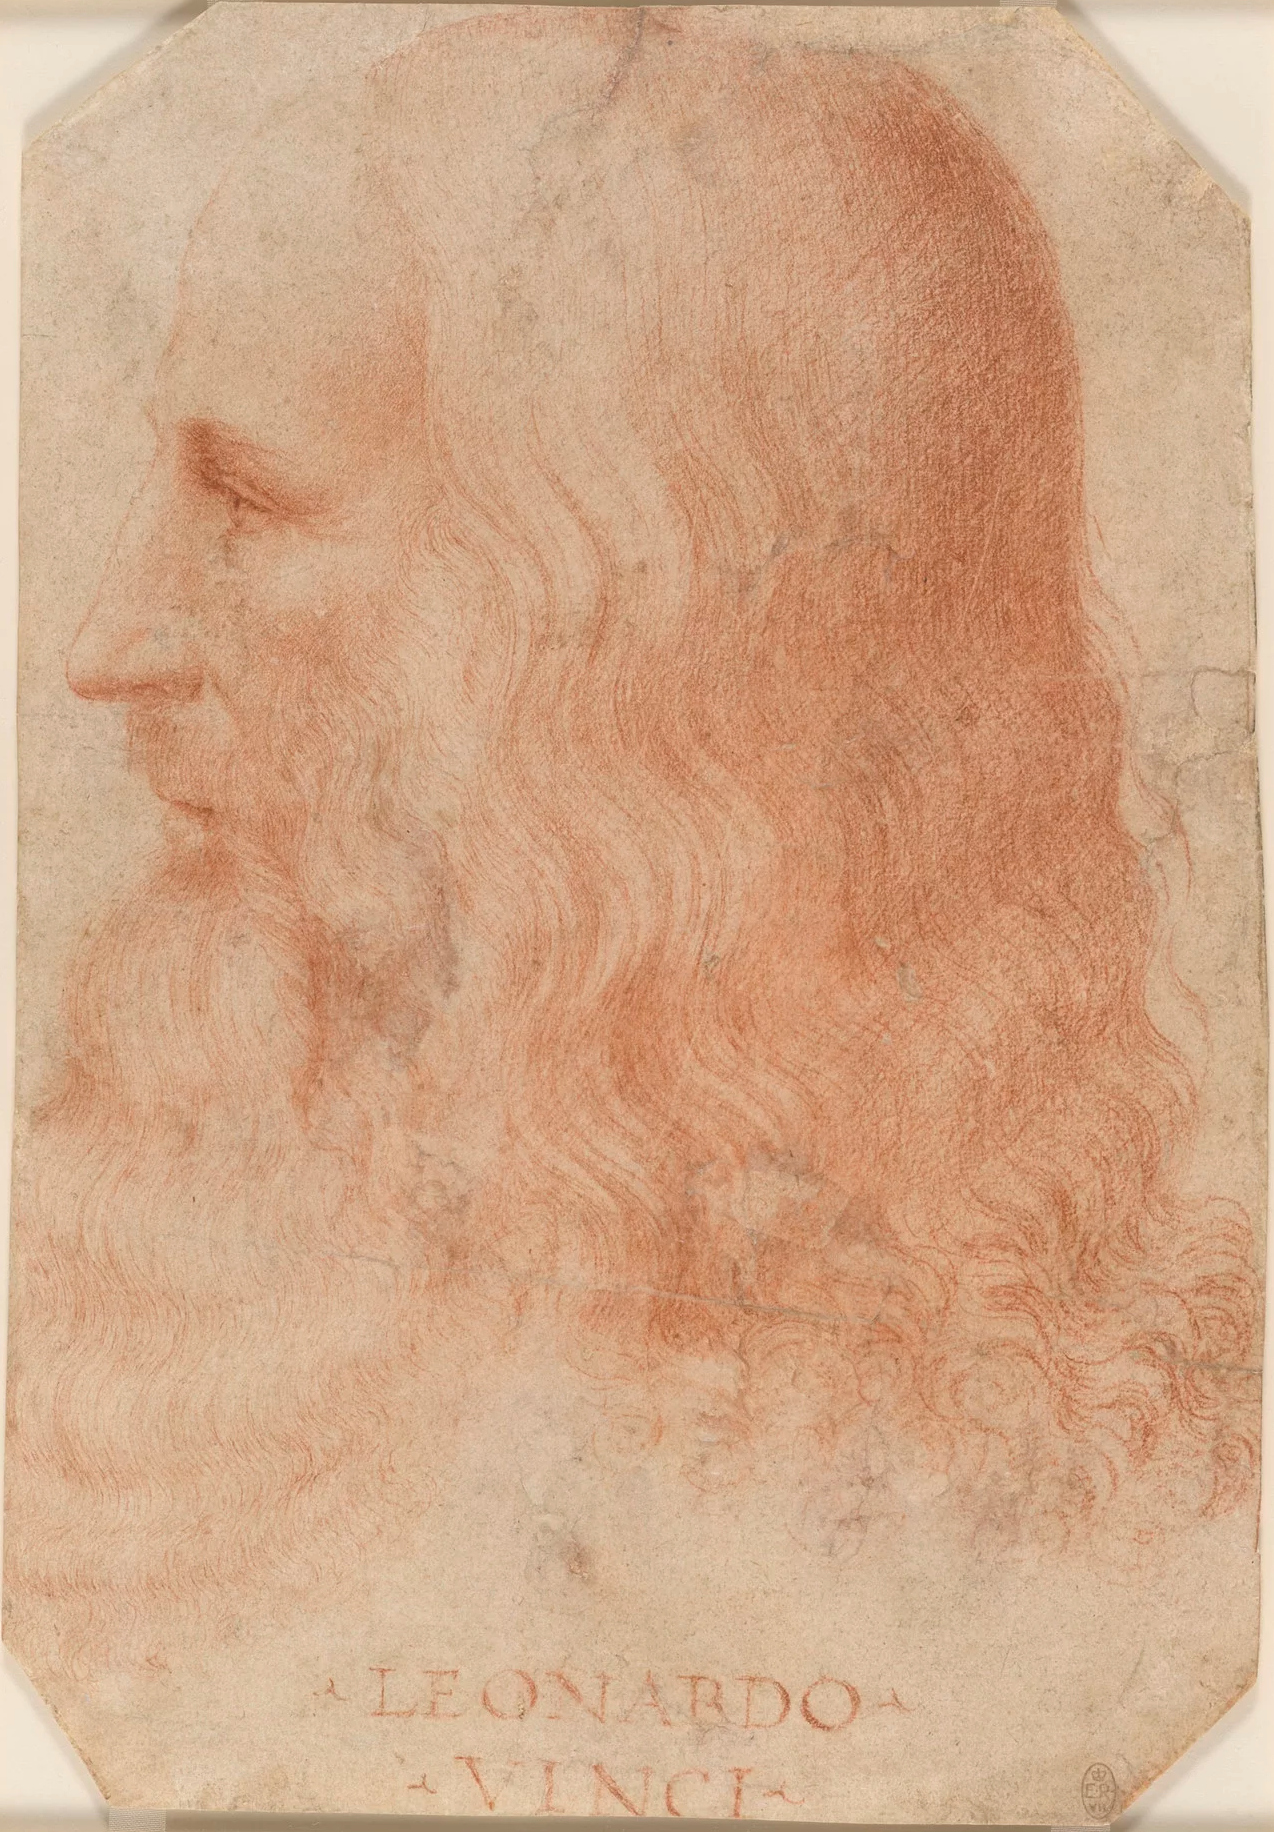
\includegraphics[height=1.65in]{images/leonardo-melzi.jpg}\par\smallskip
\small Leonardo da Vinci (1452--1519). Portrait attributed to his pupil
Francesco Melzi, Royal Collection.
\href{https://commons.wikimedia.org/wiki/File:A_portrait_of_Leonardo,_by_Francesco_Melzi.jpg}{Wikimedia Commons; public domain.}
\end{minipage}
\caption{Optics and pictorial perspective study a common geometry:
how points in space correspond to points in an image.}
\label{fig:geo-optics-portraits}
\end{figure}

\paragraph{Brunelleschi's experiment: testing a picture against the world}
\label{sec:geo-brunelleschi}

Can we test whether a picture gives the same view as the scene it depicts?
In Florence, Filippo Brunelleschi devised a striking demonstration, commonly
placed around 1415--1420. He painted the Baptistery as seen from a particular
position at the entrance to the cathedral opposite it. A small hole through
the panel allowed a viewer to look from behind the painting towards a mirror
held in front of its painted face. The mirror showed the painting's reflection;
moving it aside revealed the building itself. The viewer could compare the
two views while keeping the eye in the prescribed position.\footnote{The panel
has not survived, and its precise date and construction remain debated. A
later account by Antonio Manetti describes the hole and mirror. See Michael
Kubovy, \href{https://www.webexhibits.org/arrowintheeye/brunelleschi1.html}
{\emph{The Arrow in the Eye}, Chapter III}.}


\begin{figure}[htbp]
\centering
\begin{minipage}[t]{.46\textwidth}
\centering\vspace{0pt}
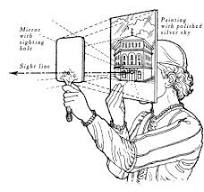
\includegraphics[width=.88\linewidth]{images/brunelleschi-mirror.jpeg}
\end{minipage}\hfill
\begin{minipage}[t]{.46\textwidth}
\centering\vspace{0pt}
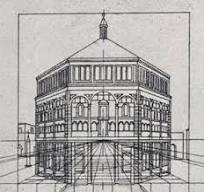
\includegraphics[width=.88\linewidth]{images/brunelleschi-baptistery.jpeg}
\end{minipage}
\caption{Brunelleschi's perspective experiment. Left: a reconstruction
showing the viewer looking through the painted panel towards a mirror.
Right: a perspective drawing of the Florentine Baptistery.
The mirror lets the viewer compare the painted view with the building
from a fixed position.}
\label{fig:geo-brunelleschi-mirror}
\end{figure}

The small hole matters because perspective depends on the position of the
eye. A picture constructed for one viewpoint need not agree with the scene
when viewed from another. This connects the experiment to our camera model:
both organise the scene around a single centre of projection. However,
Brunelleschi's hole fixed the viewing position; it did not project an image
onto a screen as a pinhole camera does. His demonstration made perspective
something that could be checked against observation.

Watch \href{https://youtu.be/bkNMM8uiMww}{\emph{Linear Perspective:
Brunelleschi's Experiment}} for a reconstruction of the arrangement.
As you watch, ask: what would change if the viewer moved sideways?


Leonardo da Vinci studied light, vision, and perspective, and used linear
perspective to organise painted space. In \emph{The Last Supper}, the
receding architectural lines help create the impression that a flat wall
opens into a room. In a perspective construction, one imagines straight
lines from the scene to a fixed eye and marks where they cross a picture
plane: the same geometric arrangement as our point-camera model.\footnote{See the
\href{https://cenacolovinciano.org/en/story/a-powerful-theatrical-machine/}{Museo del Cenacolo Vinciano's discussion of perspective in \emph{The Last Supper}}.
The use of linear perspective is distinct from evidence of tracing a
particular painting with an optical device.}

Later camera obscuras often used lenses to admit more light and mirrors
to redirect the image, and became aids to drawing. A smartphone likewise
uses lenses and a sensor, rather than a literal pinhole. Nevertheless,
central projection remains a useful geometric model when lens distortion
is negligible or corrected. The camera makes an image from a scene; our
measurement problem uses known features of the scene to reason back from
the image.

\paragraph{The problem.}
A single photograph shows two vertical objects standing on the same flat,
horizontal ground. One has known height $h_0>0$; the other has unknown
height $h>0$. Their tops and feet are visible. Four marked ground points
are also visible, and their positions on a ground plane are known.
Determine $h$ without measuring the camera's height. For this construction,
assume that the camera is higher than both objects, that neither stands
directly below it, and that their feet and the point below the camera are
not collinear. We will explain why these assumptions are useful.

\paragraph{What does an image point tell us?}
A pixel identifies a viewing line through the camera centre, not a unique
point in space. Every point on that line projects to the same image
position. However, if we know that a point lies on the ground plane, the
intersection of its viewing line with that plane locates it.

For now, suppose a function $H$ performs this intersection calculation:
\[
H(x,y)=\text{the ground coordinates corresponding to image position }(x,y).
\]
We will construct $H$ from the four marked points later. It maps positions
in the photograph to positions on a plan of the ground. It does not
recover the height of an arbitrary object by itself.

Let $C$ be the camera centre and $O$ its vertical projection onto the
ground. Write $c=CO$ for the camera height. Let $T$ and $F$ be the top
and foot of the unknown object, and let $t,f$ be their image positions. We avoid the image inversion problem by considering an equivalent virtual image plane  at the same distance in front of the camera, Convince yourself that the similar triangle relations hold.
Then
\[
H(f)=F,\qquad H(t)=R.
\]
Here $R$ is where the line from $C$ through $T$, continued beyond $T$,
meets the ground. \emph{Mapping the image of the top does not give the
foot.} It gives a different point on the same viewing line. The assumption
$c>h$ ensures that this line meets the ground beyond the object. However, convince yourself that this is not strictly required.

\begin{figure}[htbp]\centering
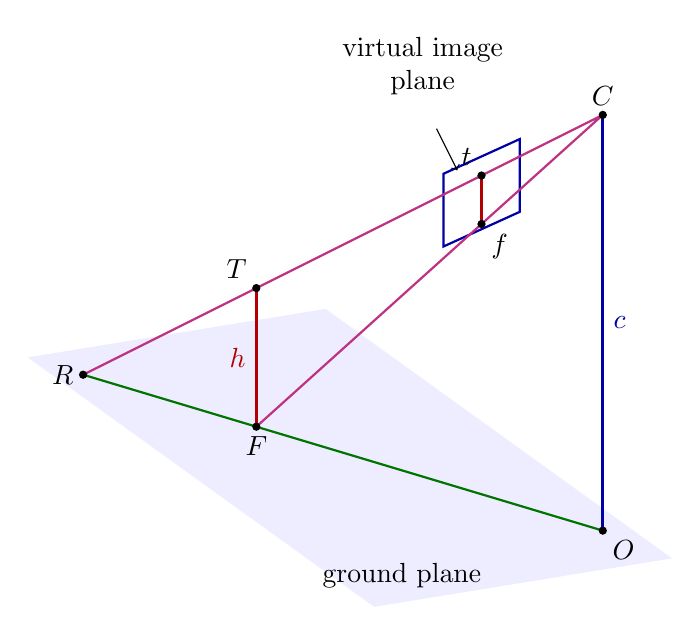
\begin{tikzpicture}[scale=.88]
\fill[blue!7] (-.3,2.5)--(4,3.2)--(9,-.4)--(4.7,-1.1)--cycle;
\coordinate (C) at (8,6);\coordinate (O) at (8,0);
\coordinate (F) at (3,1.5);\coordinate (T) at (3,3.5);
\coordinate (R) at (.5,2.25);\coordinate (t) at (6.25,5.125);\coordinate (f) at (6.25,4.425);
\draw[very thick,blue!65!black] (C)--node[right]{$c$}(O);
\draw[very thick,red!70!black] (F)--node[left]{$h$}(T);
\draw[thick,green!45!black] (R)--(O);
\draw[fill=white,fill opacity=.7,draw=blue!65!black,thick] (5.7,4.1)--(6.8,4.6)--(6.8,5.65)--(5.7,5.15)--cycle;
\draw[thick,magenta!75!black] (C)--(R) (C)--(F);
\draw[very thick,red!70!black] (t)--(f);
\foreach \p/\lab/\pos in {C/C/above,O/O/below right,F/F/below,T/T/above left,R/R/left,t/t/above left,f/f/below right}{\fill (\p) circle(1.7pt) node[\pos]{$\lab$};}
\node[above,align=center] at (5.4,6.15) {virtual image\\plane};
\draw[->] (5.6,5.8)--(5.9,5.2);
\node at (5.1,-.65) {ground plane};
\end{tikzpicture}
\caption{A spatial view of the construction, redrawn from the supplied
metrology sketch. The viewing lines through image points $t,f$ meet the
ground at $R,F$. The camera centre $C$ is vertically above $O$.
The image plane shown in front of $C$ is a convenient \emph{virtual}
plane, not the physical sensor behind the opening.}
\label{fig:geo-camera-spatial}
\end{figure}

For drawing purposes we may place an imaginary image plane in front of
$C$, where it cuts the viewing lines before they reach the scene. This
gives an upright image and simplifies the diagram. Moving to this virtual
plane does not change the viewing lines or their ground intersections.
The physical pinhole image in Figure~\ref{fig:geo-pinhole} is on the other
side of $C$ and is inverted. Figure~\ref{fig:geo-camera-triangles} isolates
the vertical cross-section that we need for the proof.

\begin{figure}[htbp]\centering
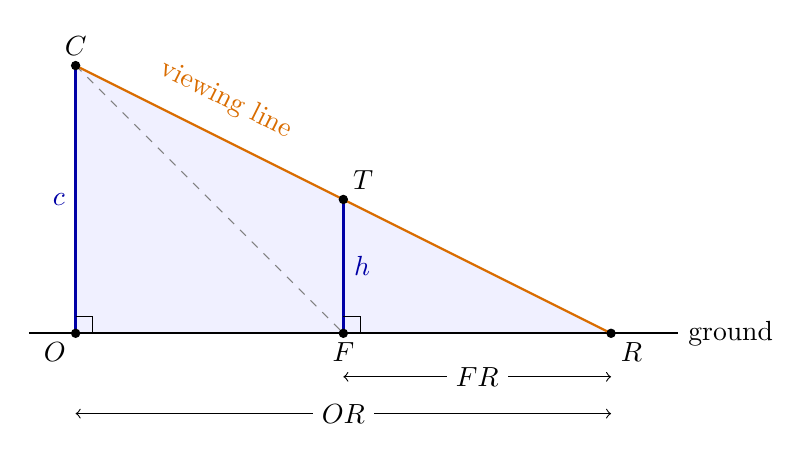
\begin{tikzpicture}[scale=.85]
\coordinate (O) at (0,0);\coordinate (C) at (0,4);
\coordinate (F) at (4,0);\coordinate (T) at (4,2);\coordinate (R) at (8,0);
\fill[blue!6] (O)--(C)--(R)--cycle;
\draw[thick] (-.7,0)--(9,0) node[right]{ground};
\draw[very thick,blue!65!black] (O)--node[left]{$c$}(C);
\draw[very thick,blue!65!black] (F)--node[right]{$h$}(T);
\draw[thick,orange!85!black] (C)--node[pos=.25,above=5pt,sloped]{viewing line}(R);
\draw[dashed,gray] (C)--(F);
\draw (0,.25)--(.25,.25)--(.25,0);
\draw (4,.25)--(4.25,.25)--(4.25,0);
\foreach \p/\lab/\pos in {O/O/below left,C/C/above,F/F/below,T/T/above right,R/R/below right}{\fill (\p) circle(2pt) node[\pos]{$\lab$};}
\draw[<->] (4,-.65)--node[fill=white]{$FR$}(8,-.65);
\draw[<->] (0,-1.2)--node[fill=white]{$OR$}(8,-1.2);
\end{tikzpicture}
\caption{A vertical cross-section through the camera and the object.
The image of the foot maps to $F$; the image of the top maps to $R$.
The right triangles $TFR$ and $COR$ are similar. The image plane is omitted
so that the geometry of the measurement is visible.}
\label{fig:geo-camera-triangles}
\end{figure}

The triangles $TFR$ and $COR$ share the angle at $R$ and each has a right
angle. Consequently,
\[
\frac{h}{c}=\frac{FR}{OR},\qquad h=c\,\frac{FR}{OR}.
\]
The lengths on the right are distances on the ground plane, after applying
$H$. Ratios of uncorrected pixel distances generally do not give the same answer.

\paragraph{Finding the point below the camera.}
For the reference object, write $F_0=H(f_0)$ and $R_0=H(t_0)$, using its
foot and top image positions. The camera and each vertical object lie in
a vertical plane. That plane meets the ground in a line through $O$.
Thus $O,F,R$ are collinear, and so are $O,F_0,R_0$. Draw the two full lines:
\[
O=\operatorname{line}(F,R)\cap\operatorname{line}(F_0,R_0).
\]
This explains the noncollinearity assumption in the problem: the two
lines must be distinct to determine their intersection. $O$ need not
lie inside the photographed patch of ground.

\begin{figure}[htbp]\centering
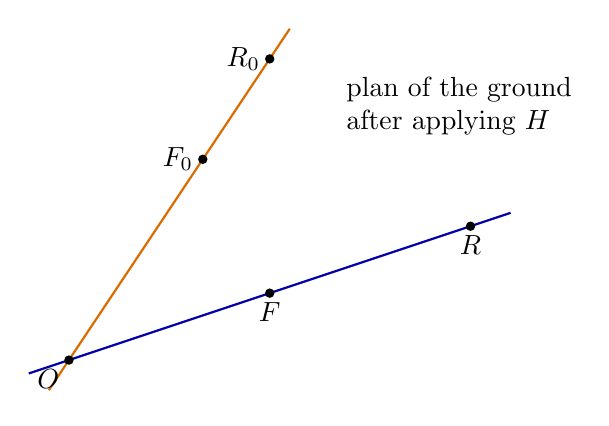
\begin{tikzpicture}[scale=.85]
\coordinate (O) at (0,0);\coordinate (F) at (3,1);\coordinate (R) at (6,2);
\coordinate (Fz) at (2,3);\coordinate (Rz) at (3,4.5);
\draw[thick,blue!65!black] (-.6,-.2)--(6.6,2.2);
\draw[thick,orange!85!black] (-.3,-.45)--(3.3,4.95);
\foreach \p/\lab/\pos in {O/O/below left,F/F/below,R/R/below,Fz/F_0/left,Rz/R_0/left}{\fill (\p) circle(2pt) node[\pos]{$\lab$};}
\node[right,align=left] at (4,3.8) {plan of the ground\\after applying $H$};
\end{tikzpicture}
\caption{Two vertical objects locate the point $O$ below the camera.
Join each mapped foot to its mapped top and extend the lines to meet.
These are ground-plane lines, not the vertical objects themselves.}
\label{fig:geo-camera-plan}
\end{figure}

\paragraph{Eliminating the camera height.}
The reference object gives another pair of similar triangles, so
\[
\frac{h_0}{c}=\frac{F_0R_0}{OR_0}.
\]
Dividing the equation for the unknown object by this equation eliminates
$c$:
\[
\boxed{h=h_0\,\frac{FR/OR}{F_0R_0/OR_0}.}
\]
For example, if $FR/OR=0.6$, $F_0R_0/OR_0=0.4$, and $h_0=1$ metre,
then $h=1.5$ metres. Multiplying every ground-plan length by the same
scale factor changes neither ratio. Thus an absolute ground-distance scale
is unnecessary once a reference height is supplied. Note, that if $H$ is known then no measurements on ground are necessary.

\paragraph{Four points straighten the ground plane.}
How do we obtain $H$? Imagine marking a rectangle on the ground and
photographing it at an angle. Its image usually looks like a quadrilateral:
parallel sides may appear to converge. Suppose we know which image corner
corresponds to each corner of the rectangle. We seek a mapping that sends
those four image positions back to their positions on the ground plane.
The required mapping is a \emph{homography}, or plane perspective
transformation. It preserves straight lines, but generally not lengths,
angles, or parallelism.

\begin{figure}[htbp]\centering
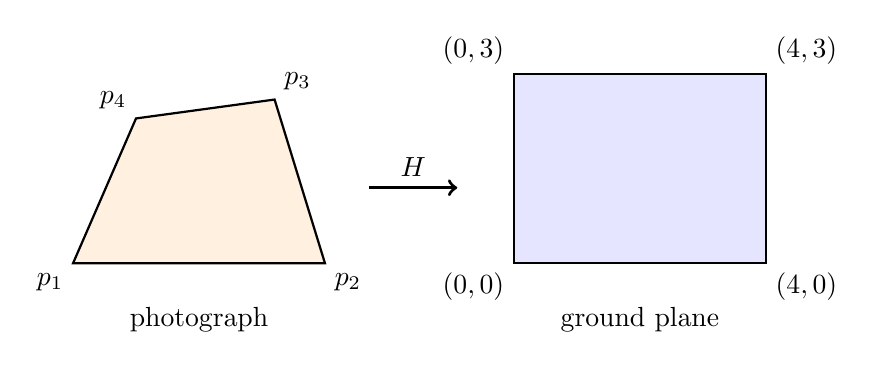
\begin{tikzpicture}[scale=.8]
\begin{scope}
\filldraw[fill=orange!12,thick] (0,0)--(4,0)--(3.2,2.6)--(1,2.3)--cycle;
\node[below left] at (0,0) {$p_1$};\node[below right] at (4,0) {$p_2$};
\node[above right] at (3.2,2.6) {$p_3$};\node[above left] at (1,2.3) {$p_4$};
\node at (2,-.9) {photograph};
\end{scope}
\draw[very thick,->] (4.7,1.2)--node[above]{$H$}(6.1,1.2);
\begin{scope}[xshift=7cm]
\filldraw[fill=blue!10,thick] (0,0) rectangle (4,3);
\node[below left] at (0,0) {$(0,0)$};\node[below right] at (4,0) {$(4,0)$};
\node[above right] at (4,3) {$(4,3)$};\node[above left] at (0,3) {$(0,3)$};
\node at (2,-.9) {ground plane};
\end{scope}
\end{tikzpicture}
\caption{Four correspondences calibrate the mapping:
$p_1\mapsto(0,0)$, $p_2\mapsto(4,0)$, $p_3\mapsto(4,3)$,
$p_4\mapsto(0,3)$. The ground coordinates must describe the marked
points; they cannot be assigned arbitrarily to four unrelated clicks.}
\label{fig:geo-homography}
\end{figure}

Four pairs of corresponding points determine a homography, provided the
points are distinct and no three are collinear in either plane. For our
rectangle, measure its side lengths or their ratio and use coordinates
such as $(0,0),(4,0),(4,3),(0,3)$. Click the four image corners in the
matching order. A supplied computational procedure finds the mapping.
It can then be evaluated at the top and foot image positions, including
positions outside the calibration quadrilateral where the mapping is finite.
The four points calibrate the ground mapping; the vertical objects supply
the additional information needed to measure height.\footnote{The familiar
perspective correction in a document-scanning application uses the same
idea: map the photographed page corners to a rectangle. See
\href{https://docs.opencv.org/4.0.0-alpha/d9/dab/tutorial_homography.html}{OpenCV's introduction to homography}.
For the broader subject, see
\href{https://visionbook.mit.edu/3d_scene_understanding_single_view.html}{\emph{Foundations of Computer Vision}, ``Single View Metrology.''}}

\paragraph{An optional algebraic glimpse.}
In suitable image coordinates, the mapping can be written
\[
H(x,y)=\left(
\frac{a_1x+a_2y+a_3}{c_1x+c_2y+1},\quad
\frac{b_1x+b_2y+b_3}{c_1x+c_2y+1}
\right).
\]
There are eight coefficients. A correspondence $(x_i,y_i)\mapsto(X_i,Y_i)$
gives two equations; for example,
\[
a_1x_i+a_2y_i+a_3=X_i(c_1x_i+c_2y_i+1),
\]
and similarly for $Y_i$. Since all four coordinates in a correspondence
are known, these are linear equations in the unknown coefficients. Four
pairs give eight equations. Under the stated conditions they determine
the mapping. We can use this computation without developing its full
algebra here. A zero denominator represents a viewing line parallel to
the ground, for which no finite ground intersection exists.

\paragraph{From the proof to a procedure.}
First calibrate $H$ using the four ground correspondences. Click the top
and foot of each object, and map those four positions with $H$. Intersect
the two mapped top--foot lines to obtain $O$. Calculate the two distance
ratios and multiply their quotient by the known height $h_0$. Every step
has a purpose supplied by the geometric argument.

\paragraph{What can go wrong?}
All clicks and calibration points must refer to the same camera view.
The model assumes a point camera with negligible or corrected lens
distortion, a flat ground plane, and truly vertical objects. If the two
ground lines nearly coincide, their intersection is poorly determined.
If a top is near camera height, its viewing line is nearly parallel to
the ground and its mapped position can be very far away: small clicking
errors may then produce large height errors. More calibration points can
help check a fitted mapping, but do not correct a wrong geometric model.
These are the same questions about assumptions and uncertainty that arose
when we measured shadows.

\subsection{Across a river, without crossing it}
\paragraph{The problem.}
Determine the perpendicular distance $AT$ to a visible but inaccessible
landmark $T$, using only constructions and length measurements on the
accessible side of a straight baseline through $A$. Assume level terrain
and unobstructed sight lines. Specify which accessible lengths suffice.

Choose a landmark $T$ on the opposite bank and a point $A$ on our bank
so that $AT$ is perpendicular to an accessible baseline. We want the
length $AT$; it need not be the river's width everywhere.
Choose $B$ along the baseline, and continue in the same direction to $C$
with $AB=BC$. From $C$ walk along a perpendicular, away from the river,
until a point $D$ is reached such that $D,B,T$ lie on one straight line.
All walking and tape measurements take place on our side.

\begin{figure}[htbp]\centering
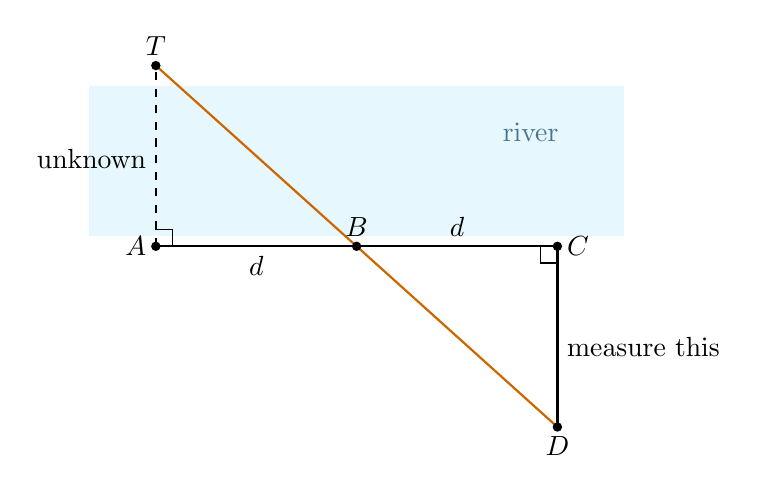
\begin{tikzpicture}[scale=.85]
\fill[cyan!10] (-1,.15) rectangle (7,2.4);
\node[cyan!50!black] at (5.6,1.7) {river};
\coordinate (A) at (0,0);\coordinate (B) at (3,0);\coordinate (C) at (6,0);
\coordinate (T) at (0,2.7);\coordinate (D) at (6,-2.7);
\draw[thick] (A)--(C)--(D);\draw[dashed,thick] (A)--(T);\draw[orange!80!black,thick] (T)--(D);
\draw (0,.25)--(.25,.25)--(.25,0);\draw (5.75,0)--(5.75,-.25)--(6,-.25);
\foreach \p/\pos in {A/left,B/above,C/right,T/above,D/below}{\fill (\p) circle(2pt);\node[\pos] at (\p){$\p$};}
\node[below] at (1.5,0) {$d$};\node[above] at (4.5,0) {$d$};
\node[left] at (0,1.3) {unknown};\node[right] at (6,-1.5) {measure this};
\end{tikzpicture}
\caption{The right triangles $TAB$ and $DCB$ are similar. Equal baseline segments make their corresponding heights equal.}
\end{figure}

The angles at $B$ are vertically opposite, and the angles at $A$ and $C$
are right angles. Similarity therefore gives
\[
\frac{AT}{CD}=\frac{AB}{BC}=1.
\]
Thus measuring $CD$ determines $AT$. If equal baseline segments are
inconvenient, the same proof gives $AT=CD\,(AB/BC)$.
The construction assumes enough clear ground behind $C$ and a visible
line of sight to $T$.\footnote{A useful geometric construction converts an
inaccessible measurement into an accessible one. Its proof also explains
which field conditions are essential: here, the two perpendiculars,
the baseline ratio, and the alignment of $T,B,D$.}

\section{Measuring the Earth: shadows, angles, and a long journey}
\label{sec:geo-earth}
Our shadow calculation treated the ground as flat and vertical sticks as
parallel. Over a small region this is a useful approximation. Over a long
north--south journey, however, the direction of the local vertical changes.
On a spherical Earth, vertical sticks point along radii from the centre.
That change of direction allows us to measure the size of the Earth without
travelling all the way around it.

In the third century BCE, Eratosthenes used observations associated with
Alexandria and Syene, near present-day Aswan in Egypt, to estimate Earth's
circumference. Before following the argument, we need a way to describe
positions on a sphere.\footnote{Eratosthenes' own account is lost. The
familiar Alexandria--Syene construction comes through later writers,
including Cleomedes. We present its idealised geometry rather than a
reconstruction of every historical observation. See
\href{https://old.maa.org/press/periodicals/convergence/eratosthenes-and-the-mystery-of-the-stades-the-basic-problem}{the Mathematical Association of America's historical discussion}.}

\begin{figure}[htbp]\centering
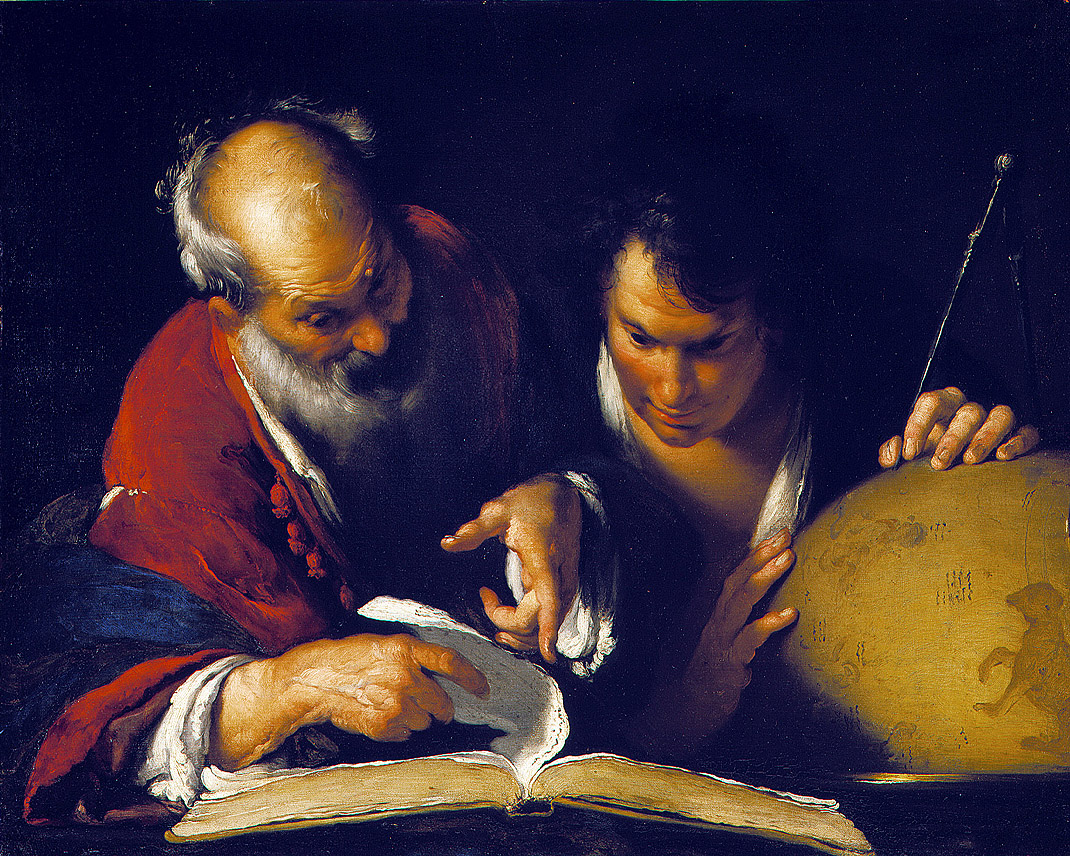
\includegraphics[width=.60\textwidth]{images/eratosthenes-strozzi.jpg}
\caption{\emph{Eratosthenes Teaching in Alexandria}, Bernardo Strozzi, 1635.
Montreal Museum of Fine Arts. This much later painting is an imaginative
representation, not a contemporary likeness.
\href{https://commons.wikimedia.org/wiki/File:Eratosthenes_Teaching_in_Alexandria_(Bernardo_Strozzi,_Montreal).jpg}{Image source: Wikimedia Commons; public domain.}}
\label{fig:geo-eratosthenes-portrait}
\end{figure}

\paragraph{The problem.}
Assume Earth is a sphere and that two observation sites lie on the same
meridian. Given their surface separation $d>0$ and the angle
$0<\theta<180^\circ$ between their local verticals, determine Earth's
great-circle circumference $C$. Explain how solar observations can supply
$\theta$ and what ground measurement is still required.

\subsection{Latitude and longitude: angles that locate a place}
Imagine Earth as a sphere with centre $O$, turning about the line joining
the North and South Poles. The plane through $O$ perpendicular to this
axis cuts the sphere in the \emph{equator}. Its latitude is $0^\circ$.

The \emph{latitude} of a point $P$ is the angle its radius $OP$ makes
with the equatorial plane. We specify north or south: the North Pole has
latitude $90^\circ$ N, the South Pole $90^\circ$ S. Points of equal latitude
form circles called \emph{parallels}. Apart from the equator, these circles
are smaller than a great circle, which is a circle whose centre is $O$.

A \emph{meridian} is a semicircle running from the North Pole to the South
Pole. Choose one as the \emph{prime meridian}. The \emph{longitude} of a
point is the angle from that reference meridian to its own, measured east
or west about Earth's rotation axis. We use $0^\circ$ to $180^\circ$ E or W;
$180^\circ$ E and $180^\circ$ W describe the same meridian. At a pole all
meridians meet, so longitude does not distinguish a position there.

\begin{figure}[htbp]\centering
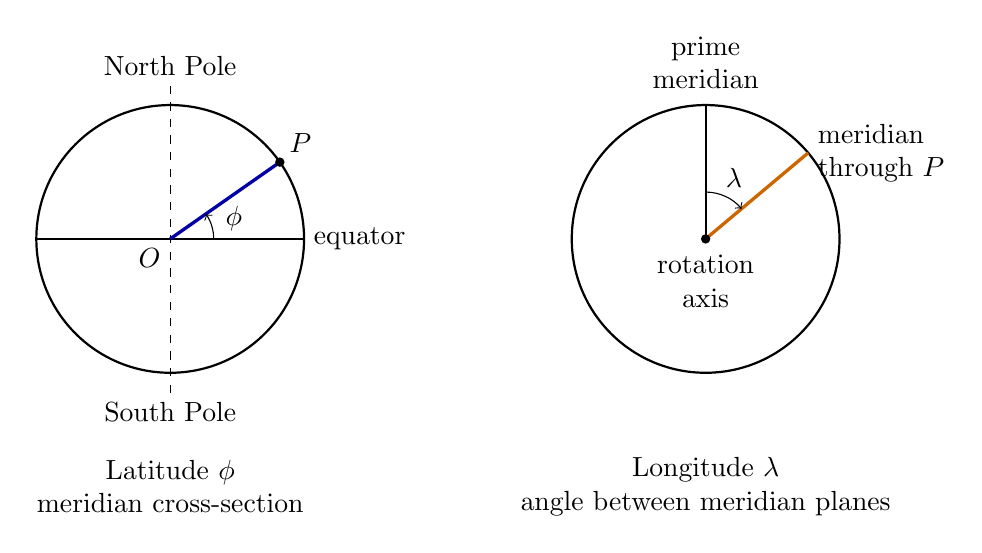
\begin{tikzpicture}[scale=.85]
\begin{scope}
\draw[thick] (0,0) circle(2);
\draw[dashed] (0,-2.3)--(0,2.3);\draw[thick] (-2,0)--(2,0);
\draw[very thick,blue!65!black] (0,0)--(35:2);
\draw[->] (.65,0) arc(0:35:.65);\node at (18:1) {$\phi$};
\fill (35:2) circle(2pt) node[above right]{$P$};
\node[below left] at (0,0) {$O$};\node[above] at (0,2.3) {North Pole};
\node[below] at (0,-2.3) {South Pole};\node[right] at (2,0) {equator};
\node[align=center] at (0,-3.7) {Latitude $\phi$\\meridian cross-section};
\end{scope}
\begin{scope}[xshift=8cm]
\draw[thick] (0,0) circle(2);
\draw[thick] (0,0)--(0,2);\draw[very thick,orange!80!black] (0,0)--(40:2);
\draw[->] (0,.7) arc(90:40:.7);\node at (65:1) {$\lambda$};
\fill (0,0) circle(2pt);\node[below,align=center] at (0,-.1) {rotation\\axis};
\node[above,align=center] at (0,2.1) {prime\\meridian};
\node[right,align=left] at (40:2) {meridian\\through $P$};
\node[align=center] at (0,-3.7) {Longitude $\lambda$\\angle between meridian planes};
\end{scope}
\end{tikzpicture}
\caption{Two separate views define the two angles. Left: a slice through the poles and $P$. Right: a view along the rotation axis; each meridian plane is represented by a radial line. The chosen angular separation is illustrative.}
\label{fig:geo-latlong}
\end{figure}

For example, $30^\circ$ N, $20^\circ$ E specifies a point north of the
equator on the meridian $20^\circ$ east of the reference. These are angles,
not distances in kilometres. A degree of longitude spans a smaller distance
along a parallel near a pole than it does at the equator, because the
parallel itself is smaller.\footnote{The modern reference for longitude
is associated with Greenwich. Unlike the equator, this reference is a
human choice, not a feature singled out by the rotation axis. Our latitude
is defined for a sphere; precise surveying accounts for Earth's flattening.
See NOAA's explanations of
\href{https://oceanservice.noaa.gov/facts/latitude.html}{latitude} and
\href{https://oceanservice.noaa.gov/facts/longitude.html}{longitude}.}

If two places lie on the same meridian, their north--south surface
separation is an arc of a great circle. The angle it subtends at the centre
is the difference of their signed latitudes. Thus two points at $24^\circ$ N
and $31^\circ$ N on the same meridian are separated by $7^\circ$ of arc.
If their longitudes differ as well, latitude difference alone does not give
the angle between their radii. This is why the north--south alignment
matters in the following argument.

\subsection{From a shadow angle to a central angle}
The idealised account begins at \emph{local solar noon} on the northern
summer solstice. Solar noon means the Sun's daily passage across the local
meridian; it need not occur at 12 on a civil clock. At Syene the Sun was
reported directly overhead: a vertical stick had no shadow. At Alexandria,
farther north, a vertical stick did cast a shadow. The stick made an
angle of about $7.2^\circ$ with the incoming sunlight.

We make three geometric assumptions: Earth is spherical, sunlight reaches
the two sites in parallel rays, and the sites lie on the same meridian.
In this idealisation they share solar noon. The overhead ray at Syene
lies along the local radius. Because the ray at Alexandria is parallel
to it, the angle between that ray and Alexandria's vertical is equal to
the angle between the two radii at Earth's centre.

\begin{figure}[htbp]\centering
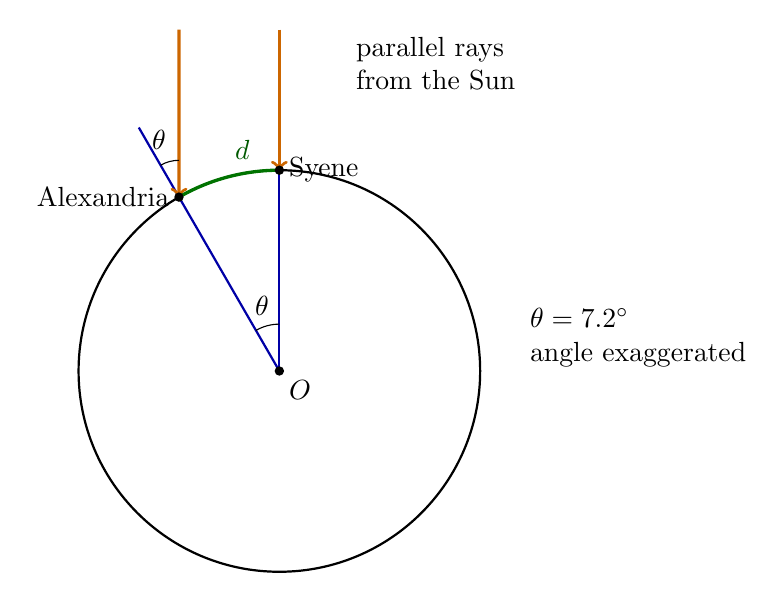
\begin{tikzpicture}[scale=.85]
\coordinate (O) at (0,0);\coordinate (S) at (0,3);\coordinate (A) at (120:3);
\draw[thick] (O) circle(3);
\draw[blue!65!black,thick] (O)--(120:4.2);\draw[blue!65!black,thick] (O)--(0,4.2);
\draw[orange!80!black,very thick,->] (0,5.1)--(S);
\draw[orange!80!black,very thick,->] (-1.5,5.1)--(A);
\draw[very thick,green!45!black] (90:3) arc(90:120:3);
\draw (90:.7) arc(90:120:.7);\node at (105:1) {$\theta$};
\draw (-1.5,3.148) arc(90:120:.55);\node at (-1.8,3.45) {$\theta$};
\fill (O) circle(2pt) node[below right]{$O$};
\fill (S) circle(2pt) node[right]{Syene};\fill (A) circle(2pt) node[left]{Alexandria};
\node[right,align=left] at (1,4.6) {parallel rays\\from the Sun};
\node[above right,green!35!black] at (105:3.12) {$d$};
\node[right,align=left] at (3.6,.5) {$\theta=7.2^\circ$\\angle exaggerated};
\end{tikzpicture}
\caption{The shadow angle measures the turn between local verticals. The surface distance $d$ is the arc between the sites, not the straight chord through Earth. The circle is a meridian cross-section, not a map with north at the top.}
\label{fig:geo-eratosthenes}
\end{figure}

The angle can be found from the right triangle formed by a vertical stick,
its shadow, and a ray from the Sun. Measure the stick and the shadow,
construct a similar triangle on paper, and read the angle between the
stick and the ray with a protractor. We do not need trigonometry for this
step. A report that the angle is one fiftieth of a full turn is equivalent
to $360^\circ/50=7.2^\circ$.

Let $d$ be the north--south surface distance between the sites and $C$
Earth's circumference along a great circle. Arcs of a circle are
proportional to their central angles, so
\[
\frac{d}{C}=\frac{\theta}{360^\circ},\qquad
C=\frac{360^\circ}{\theta}\,d.
\]
For $\theta=7.2^\circ$, this gives $C=50d$. The traditional distance of
$5000$ stadia therefore gives $250{,}000$ stadia for the circumference.
For a modern classroom illustration, using $d\approx800$ kilometres gives
$C\approx40{,}000$ kilometres. This rounded illustration is not an exact
conversion of the ancient unit.\footnote{The length of the stadion used
in this calculation is disputed, and ancient sources also report
$252{,}000$ stadia for Eratosthenes' result. It is better to state the
ancient result in its own units than attach a spurious exact percentage
accuracy to it. See
\href{https://mathshistory.st-andrews.ac.uk/Biographies/Eratosthenes/}{MacTutor's biography}
and the MAA discussion cited above.}

\subsection{Why did the measurement involve such a long journey?}
The shadow gives an \emph{angle}, not a length. A small globe and a large
globe can have the same angle between two radii. To determine which scale
we are dealing with, we need one measured distance on the ground. The
geometric argument removes the need to travel around the whole Earth;
it does not remove the need for a distance between separated sites.

Obtaining that distance in antiquity was a substantial surveying and travel
task, whether done for this purpose or taken from existing geographical
knowledge. A long trek could establish a baseline through measured stages
or careful pacing. Simply counting the distance along a winding road or
river would not suffice: the calculation needs the corresponding meridian
arc, so detours must be allowed for. We should not turn this practical
requirement into an unsupported claim that Eratosthenes personally walked
from Alexandria to Syene.\footnote{Accounts of how the distance was
obtained differ; the surviving evidence does not securely establish a
particular journey or a newly commissioned walking survey. For the
historical distance problem, see
\href{https://old.maa.org/press/periodicals/convergence/eratosthenes-and-the-mystery-of-the-stades-distance-from-alexandria-to-syene}{``Distance from Alexandria to Syene,'' MAA}.
The long trek explains the practical work behind a ground baseline, not
an independently established episode in Eratosthenes' life.}

There is a second reason to use widely separated sites: the signal becomes
easier to measure. On a sphere of circumference $40{,}000$ kilometres,
\[
\theta=360^\circ\frac{d}{40{,}000}.
\]
A baseline of $1$ kilometre gives only $0.009^\circ$; $100$ kilometres
gives $0.9^\circ$; $800$ kilometres gives $7.2^\circ$. A very short walk
produces almost parallel local verticals and a tiny difference of shadow
angles. A long baseline makes that difference more conspicuous.

\begin{figure}[htbp]\centering
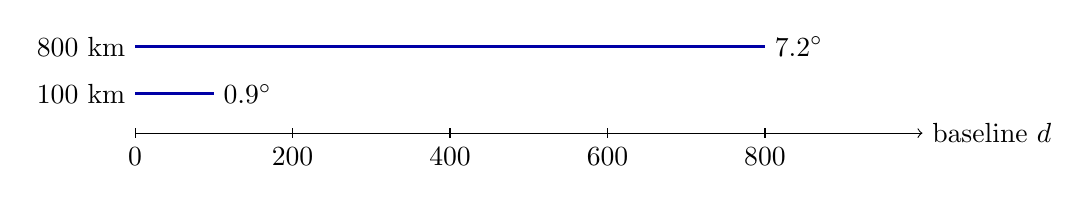
\begin{tikzpicture}[x=1cm,y=1cm]
\draw[->] (0,0)--(10,0) node[right]{baseline $d$};
\draw[very thick,blue!65!black] (0,.5)--(1,.5);
\draw[very thick,blue!65!black] (0,1.1)--(8,1.1);
\node[left] at (0,.5) {$100$ km};\node[right] at (1,.5) {$0.9^\circ$};
\node[left] at (0,1.1) {$800$ km};\node[right] at (8,1.1) {$7.2^\circ$};
\foreach \x/\lab in {0/0,2/200,4/400,6/600,8/800}{\draw (\x,.06)--(\x,-.06) node[below]{$\lab$};}
\end{tikzpicture}
\caption{On the same sphere, a longer north--south baseline produces a larger angular difference. Distances are drawn to scale; the angles are given as labels.}
\end{figure}

For example, suppose the angle can be read only within $0.1^\circ$ and
ignore distance error for the moment. With $d=800$ kilometres and a reading
of $7.2^\circ$, the possible circumference lies between
\[
\frac{360(800)}{7.3}\approx39{,}452
\quad\text{and}\quad
\frac{360(800)}{7.1}\approx40{,}563\text{ kilometres}.
\]
For $d=100$ kilometres and a reading of $0.9^\circ$, the same angular
uncertainty gives a much wider interval: $36{,}000$ to $45{,}000$ kilometres.
These are illustrative measurement bounds, not claims about the accuracy
of ancient instruments. A longer baseline helps with a fixed angular
error, but measuring that baseline introduces its own difficulties.

\subsection{What the model tells us, and what it assumes}
The cities are not exactly on the same meridian, and Syene was not exactly
at the location where the solstice Sun would be overhead. Earth is also
not a perfect sphere. These are limitations of the simplified account,
not flaws in its geometric deduction. The achievement is the method:
a terrestrial distance and an astronomical angle together determine a
planetary length scale.

Latitude makes the method especially transparent: along one meridian,
the difference in latitude is the measured central angle. Longitude tells
us why an east--west separation cannot be ignored. Places at different
longitudes generally reach solar noon at different times. Merely reading
two shadows at the same clock time need not reproduce the ideal experiment.

We have moved from a flat local model to a spherical global one. Neither
is useful at every scale. The earlier shadow calculation neglects the
change in vertical over a small area; Eratosthenes' calculation deliberately
makes that change large enough to measure.

\section{Do flights from Delhi to San Francisco fly over the pole?}
\label{sec:geo-geodesics}

\paragraph{The problem.}
Model the Earth as a sphere. What is the shortest route along its surface
from Delhi to San Francisco? Why might this route go far north, even though
neither city is close to the North Pole?

On a rectangular world map, a route curving towards the Arctic may look like
a detour. But a flat map stretches and rearranges distances on the Earth's
surface. The shortest line on the page need not represent the shortest route
on the Earth. This is another instance of a familiar question: which features
of the world does our representation preserve?

\subsection{Straight paths on curved surfaces}

On a plane, the shortest path between two points is a straight segment.
On a sphere, it is the shorter arc of a \emph{great circle}: a circle obtained
by cutting the sphere with a plane through its centre. The equator is a great
circle. A meridian together with its opposite meridian is another. Other
circles of latitude are not great circles.\footnote{For a visual explanation,
see the US Geological Survey's \href{https://www.usgs.gov/media/videos/great-circle}
{\emph{Great Circle}}.}

Such paths are examples of \emph{geodesics}, the counterpart of straight
lines on curved surfaces. A sufficiently short portion of a geodesic is a
shortest path between its endpoints. The qualification matters: going the
long way around a great circle follows a geodesic too, but is not the shortest
route between the endpoints. For two distinct points that are not opposite
one another, the shorter great-circle arc gives the unique shortest route.

Try this with a globe and a thread. Hold the ends at Delhi and San Francisco
and pull the thread taut against the surface, allowing it to settle into the
shorter route. It bends northward relative to the lines of latitude. On the
sphere, this is the direct route.

\subsection{How far north, and how far altogether?}

Use the approximate city coordinates
\[
\begin{array}{c|cc}
&\text{latitude}&\text{longitude}\\\hline
\text{Delhi}&28.6^\circ\mathrm{N}&77.2^\circ\mathrm{E}\\
\text{San Francisco}&37.8^\circ\mathrm{N}&122.4^\circ\mathrm{W}
\end{array}
\]
The smaller longitude separation is $160.4^\circ$. These points are nearly,
but not exactly, on opposite meridians. Their shorter great-circle route
reaches approximately $75.6^\circ\mathrm{N}$. It passes well into the Arctic,
but does \emph{not} pass through the North Pole.


%\begin{figure}[htbp]
%\centering
%\begin{tikzpicture}[font=\small]
%\shade[ball color=cyan!10] (0,0) circle (3);
%\draw[gray!20,densely dotted,thin] plot coordinates {(-0.5764,-0.6092) (-0.6005,-0.6170) (-0.6244,-0.6252) (-0.6481,-0.6337) (-0.6716,-0.6426) (-0.6949,-0.6517) (-0.7180,-0.6612) (-0.7409,-0.6709) (-0.7636,-0.6810) (-0.7860,-0.6913) (-0.8082,-0.7020) (-0.8301,-0.7129) (-0.8518,-0.7242) (-0.8732,-0.7357) (-0.8943,-0.7475) (-0.9152,-0.7596) (-0.9358,-0.7720) (-0.9561,-0.7846) (-0.9762,-0.7976) (-0.9959,-0.8107) (-1.0153,-0.8242) (-1.0344,-0.8379) (-1.0532,-0.8518) (-1.0717,-0.8661) (-1.0899,-0.8805) (-1.1077,-0.8952) (-1.1252,-0.9101) (-1.1423,-0.9253) (-1.1591,-0.9407) (-1.1755,-0.9563) (-1.1916,-0.9721) (-1.2073,-0.9881) (-1.2227,-1.0044) (-1.2377,-1.0208) (-1.2523,-1.0375) (-1.2665,-1.0543) (-1.2803,-1.0713) (-1.2938,-1.0885) (-1.3068,-1.1059) (-1.3195,-1.1235) (-1.3317,-1.1412) (-1.3436,-1.1591) (-1.3550,-1.1771) (-1.3660,-1.1953) (-1.3766,-1.2137) (-1.3868,-1.2321) (-1.3966,-1.2507) (-1.4059,-1.2695) (-1.4148,-1.2883) (-1.4233,-1.3073) (-1.4314,-1.3264) (-1.4390,-1.3456) (-1.4461,-1.3649) (-1.4529,-1.3842) (-1.4592,-1.4037) (-1.4650,-1.4233) (-1.4704,-1.4429) (-1.4754,-1.4626) (-1.4799,-1.4823) (-1.4839,-1.5022) (-1.4875,-1.5220) (-1.4907,-1.5419) (-1.4933,-1.5619) (-1.4956,-1.5819) (-1.4974,-1.6019) (-1.4987,-1.6219) (-1.4996,-1.6419) (-1.5000,-1.6620) (-1.4999,-1.6820) (-1.4994,-1.7021) (-1.4985,-1.7221) (-1.4970,-1.7422) (-1.4952,-1.7622) (-1.4928,-1.7821) (-1.4901,-1.8021) (-1.4868,-1.8220) (-1.4831,-1.8418) (-1.4790,-1.8616) (-1.4744,-1.8814) (-1.4694,-1.9011) (-1.4639,-1.9207) (-1.4579,-1.9402) (-1.4516,-1.9597) (-1.4447,-1.9790) (-1.4375,-1.9983) (-1.4298,-2.0175) (-1.4217,-2.0365) (-1.4131,-2.0555) (-1.4041,-2.0743) (-1.3947,-2.0930) (-1.3848,-2.1116) (-1.3745,-2.1300) (-1.3639,-2.1483) (-1.3527,-2.1665) (-1.3412,-2.1845) (-1.3293,-2.2024) (-1.3170,-2.2201) (-1.3042,-2.2376) (-1.2911,-2.2549) (-1.2776,-2.2721) (-1.2637,-2.2891) (-1.2494,-2.3059) (-1.2347,-2.3225) (-1.2197,-2.3389) (-1.2042,-2.3551) (-1.1884,-2.3711) (-1.1723,-2.3869) (-1.1558,-2.4025) (-1.1389,-2.4178) (-1.1217,-2.4329) (-1.1041,-2.4478) (-1.0863,-2.4624) (-1.0680,-2.4768) (-1.0495,-2.4910) (-1.0306,-2.5049) (-1.0115,-2.5185) (-0.9920,-2.5319) (-0.9722,-2.5451) (-0.9521,-2.5579) (-0.9317,-2.5705) (-0.9111,-2.5828) (-0.8901,-2.5949) (-0.8689,-2.6066) (-0.8475,-2.6181) (-0.8257,-2.6293) (-0.8037,-2.6402) (-0.7815,-2.6508) (-0.7591,-2.6611) (-0.7364,-2.6711) (-0.7134,-2.6808) (-0.6903,-2.6902) (-0.6670,-2.6992) (-0.6434,-2.7080) (-0.6197,-2.7164) (-0.5957,-2.7246) (-0.5716,-2.7324) (-0.5473,-2.7399) (-0.5229,-2.7470) (-0.4982,-2.7538) (-0.4735,-2.7603) (-0.4486,-2.7665) (-0.4235,-2.7723) (-0.3983,-2.7778) (-0.3730,-2.7830) (-0.3476,-2.7878) (-0.3221,-2.7923) (-0.2965,-2.7964) (-0.2708,-2.8002) (-0.2450,-2.8036) (-0.2191,-2.8068) (-0.1932,-2.8095) (-0.1672,-2.8119) (-0.1412,-2.8140) (-0.1151,-2.8157) (-0.0890,-2.8171) (-0.0628,-2.8181) (-0.0366,-2.8187) (-0.0105,-2.8190) (0.0157,-2.8190) (0.0419,-2.8186) (0.0680,-2.8179) (0.0942,-2.8168) (0.1203,-2.8154) (0.1464,-2.8136) (0.1724,-2.8115) (0.1984,-2.8090) (0.2243,-2.8062) (0.2502,-2.8030) (0.2759,-2.7995) (0.3016,-2.7956) (0.3272,-2.7914) (0.3527,-2.7869) (0.3781,-2.7820) (0.4034,-2.7767) (0.4285,-2.7712) (0.4536,-2.7653) (0.4784,-2.7591) (0.5032,-2.7525) (0.5278,-2.7456) (0.5522,-2.7384) (0.5764,-2.7308) (0.6005,-2.7230) (0.6244,-2.7148) (0.6481,-2.7063) (0.6716,-2.6975) (0.6949,-2.6883) (0.7180,-2.6789) (0.7409,-2.6691) (0.7636,-2.6591) (0.7860,-2.6487) (0.8082,-2.6380) (0.8301,-2.6271) (0.8518,-2.6158) (0.8732,-2.6043) (0.8943,-2.5925) (0.9152,-2.5804) (0.9358,-2.5680) (0.9561,-2.5554) (0.9762,-2.5425) (0.9959,-2.5293) (1.0153,-2.5158) (1.0344,-2.5021) (1.0532,-2.4882) (1.0717,-2.4740) (1.0899,-2.4595) (1.1077,-2.4448) (1.1252,-2.4299) (1.1423,-2.4147) (1.1591,-2.3994) (1.1755,-2.3838) (1.1916,-2.3679) (1.2073,-2.3519) (1.2227,-2.3356) (1.2377,-2.3192) (1.2523,-2.3026) (1.2665,-2.2857) (1.2803,-2.2687) (1.2938,-2.2515) (1.3068,-2.2341) (1.3195,-2.2165) (1.3317,-2.1988) (1.3436,-2.1809) (1.3550,-2.1629) (1.3660,-2.1447) (1.3766,-2.1264) (1.3868,-2.1079) (1.3966,-2.0893) (1.4059,-2.0705) (1.4148,-2.0517) (1.4233,-2.0327) (1.4314,-2.0136) (1.4390,-1.9944) (1.4461,-1.9752) (1.4529,-1.9558) (1.4592,-1.9363) (1.4650,-1.9168) (1.4704,-1.8971) (1.4754,-1.8774) (1.4799,-1.8577) (1.4839,-1.8379) (1.4875,-1.8180) (1.4907,-1.7981) (1.4933,-1.7781) (1.4956,-1.7582) (1.4974,-1.7382) (1.4987,-1.7181) (1.4996,-1.6981) (1.5000,-1.6780) (1.4999,-1.6580) (1.4994,-1.6379) (1.4985,-1.6179) (1.4970,-1.5979) (1.4952,-1.5779) (1.4928,-1.5579) (1.4901,-1.5379) (1.4868,-1.5180) (1.4831,-1.4982) (1.4790,-1.4784) (1.4744,-1.4586) (1.4694,-1.4390) (1.4639,-1.4194) (1.4579,-1.3998) (1.4516,-1.3804) (1.4447,-1.3610) (1.4375,-1.3417) (1.4298,-1.3226) (1.4217,-1.3035) (1.4131,-1.2846) (1.4041,-1.2657) (1.3947,-1.2470) (1.3848,-1.2284) (1.3745,-1.2100) (1.3639,-1.1917) (1.3527,-1.1735) (1.3412,-1.1555) (1.3293,-1.1377) (1.3170,-1.1200) (1.3042,-1.1024) (1.2911,-1.0851) (1.2776,-1.0679) (1.2637,-1.0509) (1.2494,-1.0341) (1.2347,-1.0175) (1.2197,-1.0011) (1.2042,-0.9849) (1.1884,-0.9689) (1.1723,-0.9531) (1.1558,-0.9376) (1.1389,-0.9222) (1.1217,-0.9071) (1.1041,-0.8922) (1.0863,-0.8776) (1.0680,-0.8632) (1.0495,-0.8490) (1.0306,-0.8351) (1.0115,-0.8215) (0.9920,-0.8081) (0.9722,-0.7950) (0.9521,-0.7821) (0.9317,-0.7695) (0.9111,-0.7572) (0.8901,-0.7451) (0.8689,-0.7334) (0.8475,-0.7219) (0.8257,-0.7107) (0.8037,-0.6998) (0.7815,-0.6892) (0.7591,-0.6789) (0.7364,-0.6689) (0.7134,-0.6592) (0.6903,-0.6499) (0.6670,-0.6408) (0.6434,-0.6320) (0.6197,-0.6236) (0.5957,-0.6154) (0.5716,-0.6076) (0.5473,-0.6002) (0.5229,-0.5930) (0.4982,-0.5862) (0.4735,-0.5797) (0.4486,-0.5735) (0.4235,-0.5677) (0.3983,-0.5622) (0.3730,-0.5570) (0.3476,-0.5522) (0.3221,-0.5477) (0.2965,-0.5436) (0.2708,-0.5398) (0.2450,-0.5364) (0.2191,-0.5333) (0.1932,-0.5305) (0.1672,-0.5281) (0.1412,-0.5260) (0.1151,-0.5243) (0.0890,-0.5230) (0.0628,-0.5220) (0.0366,-0.5213) (0.0105,-0.5210) (-0.0157,-0.5210) (-0.0419,-0.5214) (-0.0680,-0.5221) (-0.0942,-0.5232) (-0.1203,-0.5246) (-0.1464,-0.5264) (-0.1724,-0.5286) (-0.1984,-0.5310) (-0.2243,-0.5339) (-0.2502,-0.5370) (-0.2759,-0.5406) (-0.3016,-0.5444) (-0.3272,-0.5486) (-0.3527,-0.5532) (-0.3781,-0.5580) (-0.4034,-0.5633) (-0.4285,-0.5688) (-0.4536,-0.5747) (-0.4784,-0.5810) (-0.5032,-0.5875) (-0.5278,-0.5944) (-0.5522,-0.6016) (-0.5764,-0.6092)};
%\draw[gray!20,densely dotted,thin] plot coordinates {(-0.9984,0.8732) (-1.0401,0.8596) (-1.0815,0.8454) (-1.1226,0.8307) (-1.1633,0.8154) (-1.2037,0.7996) (-1.2437,0.7832) (-1.2833,0.7663) (-1.3225,0.7489) (-1.3614,0.7310) (-1.3998,0.7125) (-1.4378,0.6935) (-1.4753,0.6741) (-1.5124,0.6541) (-1.5490,0.6336) (-1.5852,0.6127) (-1.6209,0.5912) (-1.6561,0.5693) (-1.6908,0.5470) (-1.7249,0.5241) (-1.7586,0.5008) (-1.7917,0.4771) (-1.8242,0.4529) (-1.8563,0.4283) (-1.8877,0.4033) (-1.9186,0.3778) (-1.9488,0.3520) (-1.9785,0.3257) (-2.0076,0.2991) (-2.0361,0.2721) (-2.0639,0.2446) (-2.0912,0.2169) (-2.1178,0.1887) (-2.1437,0.1602) (-2.1690,0.1314) (-2.1936,0.1022) (-2.2176,0.0728) (-2.2409,0.0429) (-2.2635,0.0128) (-2.2854,-0.0176) (-2.3066,-0.0483) (-2.3271,-0.0792) (-2.3469,-0.1105) (-2.3660,-0.1420) (-2.3844,-0.1738) (-2.4020,-0.2058) (-2.4190,-0.2380) (-2.4351,-0.2704) (-2.4506,-0.3031) (-2.4653,-0.3360) (-2.4792,-0.3690) (-2.4924,-0.4023) (-2.5048,-0.4357) (-2.5165,-0.4692) (-2.5273,-0.5029) (-2.5375,-0.5368) (-2.5468,-0.5708) (-2.5554,-0.6049) (-2.5632,-0.6391) (-2.5702,-0.6734) (-2.5764,-0.7078) (-2.5819,-0.7423) (-2.5865,-0.7769) (-2.5904,-0.8115) (-2.5935,-0.8461) (-2.5958,-0.8808) (-2.5973,-0.9156) (-2.5980,-0.9503) (-2.5979,-0.9850) (-2.5971,-1.0198) (-2.5954,-1.0545) (-2.5929,-1.0891) (-2.5897,-1.1238) (-2.5857,-1.1584) (-2.5809,-1.1929) (-2.5753,-1.2274) (-2.5689,-1.2618) (-2.5617,-1.2961) (-2.5537,-1.3303) (-2.5450,-1.3644) (-2.5355,-1.3983) (-2.5252,-1.4322) (-2.5142,-1.4659) (-2.5024,-1.4994) (-2.4898,-1.5328) (-2.4765,-1.5660) (-2.4624,-1.5990) (-2.4475,-1.6318) (-2.4320,-1.6644) (-2.4156,-1.6968) (-2.3986,-1.7290) (-2.3808,-1.7610) (-2.3623,-1.7927) (-2.3430,-1.8241) (-2.3231,-1.8553) (-2.3024,-1.8863) (-2.2811,-1.9169) (-2.2590,-1.9472) (-2.2363,-1.9773) (-2.2129,-2.0070) (-2.1888,-2.0365) (-2.1640,-2.0656) (-2.1386,-2.0943) (-2.1125,-2.1227) (-2.0858,-2.1508) (-2.0584,-2.1785) (-2.0304,-2.2059) (-2.0019,-2.2328) (-1.9726,-2.2594) (-1.9428,-2.2856) (-1.9124,-2.3113)};
%\draw[gray!20,densely dotted,thin] plot coordinates {(1.8877,-2.3317) (1.9186,-2.3062) (1.9488,-2.2804) (1.9785,-2.2541) (2.0076,-2.2274) (2.0361,-2.2004) (2.0639,-2.1730) (2.0912,-2.1452) (2.1178,-2.1171) (2.1437,-2.0886) (2.1690,-2.0598) (2.1936,-2.0306) (2.2176,-2.0011) (2.2409,-1.9713) (2.2635,-1.9412) (2.2854,-1.9108) (2.3066,-1.8801) (2.3271,-1.8491) (2.3469,-1.8179) (2.3660,-1.7864) (2.3844,-1.7546) (2.4020,-1.7226) (2.4190,-1.6904) (2.4351,-1.6579) (2.4506,-1.6253) (2.4653,-1.5924) (2.4792,-1.5593) (2.4924,-1.5261) (2.5048,-1.4927) (2.5165,-1.4591) (2.5273,-1.4254) (2.5375,-1.3916) (2.5468,-1.3576) (2.5554,-1.3235) (2.5632,-1.2892) (2.5702,-1.2549) (2.5764,-1.2205) (2.5819,-1.1860) (2.5865,-1.1515) (2.5904,-1.1169) (2.5935,-1.0822) (2.5958,-1.0475) (2.5973,-1.0128) (2.5980,-0.9781) (2.5979,-0.9433) (2.5971,-0.9086) (2.5954,-0.8739) (2.5929,-0.8392) (2.5897,-0.8046) (2.5857,-0.7700) (2.5809,-0.7354) (2.5753,-0.7010) (2.5689,-0.6666) (2.5617,-0.6323) (2.5537,-0.5981) (2.5450,-0.5640) (2.5355,-0.5300) (2.5252,-0.4962) (2.5142,-0.4625) (2.5024,-0.4290) (2.4898,-0.3956) (2.4765,-0.3624) (2.4624,-0.3294) (2.4475,-0.2966) (2.4320,-0.2639) (2.4156,-0.2315) (2.3986,-0.1993) (2.3808,-0.1674) (2.3623,-0.1357) (2.3430,-0.1042) (2.3231,-0.0730) (2.3024,-0.0421) (2.2811,-0.0115) (2.2590,0.0189) (2.2363,0.0489) (2.2129,0.0787) (2.1888,0.1081) (2.1640,0.1372) (2.1386,0.1660) (2.1125,0.1944) (2.0858,0.2225) (2.0584,0.2502) (2.0304,0.2775) (2.0019,0.3044) (1.9726,0.3310) (1.9428,0.3572) (1.9124,0.3830) (1.8815,0.4083) (1.8499,0.4333) (1.8178,0.4578) (1.7851,0.4819) (1.7519,0.5055) (1.7181,0.5287) (1.6839,0.5515) (1.6491,0.5737) (1.6138,0.5956) (1.5780,0.6169) (1.5417,0.6378) (1.5050,0.6581) (1.4678,0.6780) (1.4302,0.6974) (1.3921,0.7162) (1.3536,0.7346) (1.3147,0.7524) (1.2754,0.7697) (1.2357,0.7865) (1.1956,0.8028) (1.1552,0.8185) (1.1144,0.8337) (1.0733,0.8483) (1.0318,0.8624) (0.9900,0.8759) (0.9480,0.8888) (0.9056,0.9012) (0.8630,0.9131) (0.8201,0.9243) (0.7769,0.9350) (0.7335,0.9451) (0.6899,0.9546) (0.6461,0.9635) (0.6021,0.9719) (0.5579,0.9796) (0.5135,0.9868) (0.4690,0.9934) (0.4243,0.9993) (0.3795,1.0047) (0.3346,1.0095) (0.2896,1.0137) (0.2445,1.0172) (0.1993,1.0202) (0.1541,1.0226) (0.1088,1.0243) (0.0635,1.0255) (0.0181,1.0260) (-0.0272,1.0260) (-0.0725,1.0253) (-0.1179,1.0240) (-0.1631,1.0221) (-0.2084,1.0196) (-0.2535,1.0166) (-0.2986,1.0129) (-0.3436,1.0086) (-0.3885,1.0037) (-0.4333,0.9982) (-0.4779,0.9921) (-0.5224,0.9854) (-0.5668,0.9781) (-0.6109,0.9703) (-0.6549,0.9618) (-0.6987,0.9527) (-0.7422,0.9431) (-0.7856,0.9329) (-0.8287,0.9221) (-0.8715,0.9107) (-0.9141,0.8988) (-0.9564,0.8863) (-0.9984,0.8732)};
%\draw[gray!45,thin] plot coordinates {(-1.8815,-2.3367) (-1.8499,-2.3616) (-1.8178,-2.3862) (-1.7851,-2.4102) (-1.7519,-2.4339) (-1.7181,-2.4571) (-1.6839,-2.4798) (-1.6491,-2.5021) (-1.6138,-2.5239) (-1.5780,-2.5453) (-1.5417,-2.5661) (-1.5050,-2.5865) (-1.4678,-2.6064) (-1.4302,-2.6257) (-1.3921,-2.6446) (-1.3536,-2.6630) (-1.3147,-2.6808) (-1.2754,-2.6981) (-1.2357,-2.7149) (-1.1956,-2.7311) (-1.1552,-2.7469) (-1.1144,-2.7620) (-1.0733,-2.7767) (-1.0318,-2.7907) (-0.9900,-2.8043) (-0.9480,-2.8172) (-0.9056,-2.8296) (-0.8630,-2.8414) (-0.8201,-2.8527) (-0.7769,-2.8634) (-0.7335,-2.8734) (-0.6899,-2.8830) (-0.6461,-2.8919) (-0.6021,-2.9002) (-0.5579,-2.9080) (-0.5135,-2.9152) (-0.4690,-2.9217) (-0.4243,-2.9277) (-0.3795,-2.9331) (-0.3346,-2.9378) (-0.2896,-2.9420) (-0.2445,-2.9456) (-0.1993,-2.9486) (-0.1541,-2.9509) (-0.1088,-2.9527) (-0.0635,-2.9538) (-0.0181,-2.9544) (0.0272,-2.9543) (0.0725,-2.9536) (0.1179,-2.9524) (0.1631,-2.9505) (0.2084,-2.9480) (0.2535,-2.9449) (0.2986,-2.9412) (0.3436,-2.9369) (0.3885,-2.9320) (0.4333,-2.9266) (0.4779,-2.9205) (0.5224,-2.9138) (0.5668,-2.9065) (0.6109,-2.8986) (0.6549,-2.8902) (0.6987,-2.8811) (0.7422,-2.8715) (0.7856,-2.8613) (0.8287,-2.8505) (0.8715,-2.8391) (0.9141,-2.8272) (0.9564,-2.8147) (0.9984,-2.8016) (1.0401,-2.7880) (1.0815,-2.7738) (1.1226,-2.7590) (1.1633,-2.7438) (1.2037,-2.7279) (1.2437,-2.7116) (1.2833,-2.6947) (1.3225,-2.6773) (1.3614,-2.6593) (1.3998,-2.6409) (1.4378,-2.6219) (1.4753,-2.6024) (1.5124,-2.5824) (1.5490,-2.5620) (1.5852,-2.5410) (1.6209,-2.5196) (1.6561,-2.4977) (1.6908,-2.4753) (1.7249,-2.4525) (1.7586,-2.4292) (1.7917,-2.4055) (1.8242,-2.3813) (1.8563,-2.3567)};
%\draw[gray!20,densely dotted,thin] plot coordinates {(-1.1529,2.1217) (-1.2010,2.1059) (-1.2488,2.0895) (-1.2963,2.0725) (-1.3433,2.0549) (-1.3899,2.0366) (-1.4361,2.0177) (-1.4818,1.9982) (-1.5271,1.9781) (-1.5720,1.9574) (-1.6163,1.9361) (-1.6602,1.9142) (-1.7035,1.8917) (-1.7464,1.8686) (-1.7887,1.8450) (-1.8304,1.8208) (-1.8716,1.7960) (-1.9123,1.7707) (-1.9523,1.7449) (-1.9918,1.7185) (-2.0306,1.6916) (-2.0689,1.6642) (-2.1065,1.6363) (-2.1434,1.6079) (-2.1797,1.5790) (-2.2154,1.5496) (-2.2503,1.5198) (-2.2846,1.4895) (-2.3182,1.4587) (-2.3511,1.4275) (-2.3832,1.3958) (-2.4147,1.3638) (-2.4454,1.3313) (-2.4753,1.2984) (-2.5045,1.2651) (-2.5330,1.2314) (-2.5607,1.1973) (-2.5875,1.1629) (-2.6136,1.1282) (-2.6389,1.0930) (-2.6634,1.0576) (-2.6871,1.0218) (-2.7100,0.9858) (-2.7321,0.9494) (-2.7533,0.9127) (-2.7736,0.8758) (-2.7932,0.8385) (-2.8118,0.8011) (-2.8297,0.7634) (-2.8466,0.7254) (-2.8627,0.6872) (-2.8779,0.6489) (-2.8923,0.6103) (-2.9057,0.5715) (-2.9183,0.5326) (-2.9300,0.4935) (-2.9408,0.4542) (-2.9507,0.4149) (-2.9597,0.3753) (-2.9678,0.3357) (-2.9750,0.2960) (-2.9813,0.2562) (-2.9867,0.2163) (-2.9912,0.1763) (-2.9947,0.1363) (-2.9974,0.0962) (-2.9991,0.0561) (-2.9999,0.0160)};
%\draw[gray!20,densely dotted,thin] plot coordinates {(2.9998,0.0241) (2.9988,0.0642) (2.9969,0.1043) (2.9941,0.1443) (2.9903,0.1843) (2.9857,0.2243) (2.9801,0.2641) (2.9736,0.3039) (2.9663,0.3437) (2.9580,0.3833) (2.9488,0.4227) (2.9387,0.4621) (2.9278,0.5013) (2.9159,0.5404) (2.9031,0.5793) (2.8895,0.6180) (2.8750,0.6565) (2.8596,0.6949) (2.8433,0.7330) (2.8262,0.7709) (2.8082,0.8086) (2.7893,0.8460) (2.7696,0.8832) (2.7491,0.9201) (2.7277,0.9567) (2.7055,0.9930) (2.6825,1.0290) (2.6586,1.0647) (2.6339,1.1001) (2.6085,1.1351) (2.5822,1.1698) (2.5552,1.2042) (2.5274,1.2382) (2.4988,1.2718) (2.4694,1.3050) (2.4393,1.3378) (2.4085,1.3702) (2.3769,1.4022) (2.3446,1.4338) (2.3115,1.4649) (2.2778,1.4956) (2.2434,1.5258) (2.2083,1.5556) (2.1725,1.5848) (2.1361,1.6136) (2.0990,1.6420) (2.0613,1.6698) (2.0229,1.6971) (1.9839,1.7239) (1.9444,1.7501) (1.9042,1.7758) (1.8634,1.8010) (1.8221,1.8257) (1.7803,1.8498) (1.7378,1.8733) (1.6949,1.8962) (1.6514,1.9186) (1.6075,1.9404) (1.5630,1.9616) (1.5181,1.9822) (1.4727,2.0022) (1.4269,2.0215) (1.3806,2.0403) (1.3339,2.0585) (1.2868,2.0760) (1.2393,2.0929) (1.1914,2.1091) (1.1432,2.1247) (1.0946,2.1397) (1.0457,2.1540) (0.9965,2.1677) (0.9469,2.1806) (0.8971,2.1930) (0.8470,2.2046) (0.7967,2.2156) (0.7461,2.2259) (0.6952,2.2356) (0.6442,2.2445) (0.5930,2.2528) (0.5416,2.2604) (0.4900,2.2673) (0.4382,2.2735) (0.3864,2.2790) (0.3344,2.2838) (0.2823,2.2879) (0.2302,2.2914) (0.1779,2.2941) (0.1256,2.2961) (0.0733,2.2974) (0.0209,2.2981) (-0.0314,2.2980) (-0.0838,2.2972) (-0.1361,2.2958) (-0.1884,2.2936) (-0.2406,2.2907) (-0.2927,2.2872) (-0.3448,2.2829) (-0.3968,2.2779) (-0.4486,2.2723) (-0.5003,2.2660) (-0.5519,2.2589) (-0.6032,2.2512) (-0.6544,2.2428) (-0.7054,2.2337) (-0.7562,2.2239) (-0.8068,2.2135) (-0.8571,2.2024) (-0.9071,2.1906) (-0.9569,2.1781) (-1.0064,2.1650) (-1.0555,2.1512) (-1.1044,2.1368) (-1.1529,2.1217)};
%\draw[gray!45,thin] plot coordinates {(-2.9998,-0.0241) (-2.9988,-0.0642) (-2.9969,-0.1043) (-2.9941,-0.1443) (-2.9903,-0.1843) (-2.9857,-0.2243) (-2.9801,-0.2641) (-2.9736,-0.3039) (-2.9663,-0.3437) (-2.9580,-0.3833) (-2.9488,-0.4227) (-2.9387,-0.4621) (-2.9278,-0.5013) (-2.9159,-0.5404) (-2.9031,-0.5793) (-2.8895,-0.6180) (-2.8750,-0.6565) (-2.8596,-0.6949) (-2.8433,-0.7330) (-2.8262,-0.7709) (-2.8082,-0.8086) (-2.7893,-0.8460) (-2.7696,-0.8832) (-2.7491,-0.9201) (-2.7277,-0.9567) (-2.7055,-0.9930) (-2.6825,-1.0290) (-2.6586,-1.0647) (-2.6339,-1.1001) (-2.6085,-1.1351) (-2.5822,-1.1698) (-2.5552,-1.2042) (-2.5274,-1.2382) (-2.4988,-1.2718) (-2.4694,-1.3050) (-2.4393,-1.3378) (-2.4085,-1.3702) (-2.3769,-1.4022) (-2.3446,-1.4338) (-2.3115,-1.4649) (-2.2778,-1.4956) (-2.2434,-1.5258) (-2.2083,-1.5556) (-2.1725,-1.5848) (-2.1361,-1.6136) (-2.0990,-1.6420) (-2.0613,-1.6698) (-2.0229,-1.6971) (-1.9839,-1.7239) (-1.9444,-1.7501) (-1.9042,-1.7758) (-1.8634,-1.8010) (-1.8221,-1.8257) (-1.7803,-1.8498) (-1.7378,-1.8733) (-1.6949,-1.8962) (-1.6514,-1.9186) (-1.6075,-1.9404) (-1.5630,-1.9616) (-1.5181,-1.9822) (-1.4727,-2.0022) (-1.4269,-2.0215) (-1.3806,-2.0403) (-1.3339,-2.0585) (-1.2868,-2.0760) (-1.2393,-2.0929) (-1.1914,-2.1091) (-1.1432,-2.1247) (-1.0946,-2.1397) (-1.0457,-2.1540) (-0.9965,-2.1677) (-0.9469,-2.1806) (-0.8971,-2.1930) (-0.8470,-2.2046) (-0.7967,-2.2156) (-0.7461,-2.2259) (-0.6952,-2.2356) (-0.6442,-2.2445) (-0.5930,-2.2528) (-0.5416,-2.2604) (-0.4900,-2.2673) (-0.4382,-2.2735) (-0.3864,-2.2790) (-0.3344,-2.2838) (-0.2823,-2.2879) (-0.2302,-2.2914) (-0.1779,-2.2941) (-0.1256,-2.2961) (-0.0733,-2.2974) (-0.0209,-2.2981) (0.0314,-2.2980) (0.0838,-2.2972) (0.1361,-2.2958) (0.1884,-2.2936) (0.2406,-2.2907) (0.2927,-2.2872) (0.3448,-2.2829) (0.3968,-2.2779) (0.4486,-2.2723) (0.5003,-2.2660) (0.5519,-2.2589) (0.6032,-2.2512) (0.6544,-2.2428) (0.7054,-2.2337) (0.7562,-2.2239) (0.8068,-2.2135) (0.8571,-2.2024) (0.9071,-2.1906) (0.9569,-2.1781) (1.0064,-2.1650) (1.0555,-2.1512) (1.1044,-2.1368) (1.1529,-2.1217) (1.2010,-2.1059) (1.2488,-2.0895) (1.2963,-2.0725) (1.3433,-2.0549) (1.3899,-2.0366) (1.4361,-2.0177) (1.4818,-1.9982) (1.5271,-1.9781) (1.5720,-1.9574) (1.6163,-1.9361) (1.6602,-1.9142) (1.7035,-1.8917) (1.7464,-1.8686) (1.7887,-1.8450) (1.8304,-1.8208) (1.8716,-1.7960) (1.9123,-1.7707) (1.9523,-1.7449) (1.9918,-1.7185) (2.0306,-1.6916) (2.0689,-1.6642) (2.1065,-1.6363) (2.1434,-1.6079) (2.1797,-1.5790) (2.2154,-1.5496) (2.2503,-1.5198) (2.2846,-1.4895) (2.3182,-1.4587) (2.3511,-1.4275) (2.3832,-1.3958) (2.4147,-1.3638) (2.4454,-1.3313) (2.4753,-1.2984) (2.5045,-1.2651) (2.5330,-1.2314) (2.5607,-1.1973) (2.5875,-1.1629) (2.6136,-1.1282) (2.6389,-1.0930) (2.6634,-1.0576) (2.6871,-1.0218) (2.7100,-0.9858) (2.7321,-0.9494) (2.7533,-0.9127) (2.7736,-0.8758) (2.7932,-0.8385) (2.8118,-0.8011) (2.8297,-0.7634) (2.8466,-0.7254) (2.8627,-0.6872) (2.8779,-0.6489) (2.8923,-0.6103) (2.9057,-0.5715) (2.9183,-0.5326) (2.9300,-0.4935) (2.9408,-0.4542) (2.9507,-0.4149) (2.9597,-0.3753) (2.9678,-0.3357) (2.9750,-0.2960) (2.9813,-0.2562) (2.9867,-0.2163) (2.9912,-0.1763) (2.9947,-0.1363) (2.9974,-0.0962) (2.9991,-0.0561) (2.9999,-0.0160)};
%\draw[gray!20,densely dotted,thin] plot coordinates {(-0.9984,2.8016) (-1.0401,2.7880) (-1.0815,2.7738) (-1.1226,2.7590) (-1.1633,2.7438) (-1.2037,2.7279) (-1.2437,2.7116) (-1.2833,2.6947) (-1.3225,2.6773) (-1.3614,2.6593) (-1.3998,2.6409) (-1.4378,2.6219) (-1.4753,2.6024) (-1.5124,2.5824) (-1.5490,2.5620) (-1.5852,2.5410) (-1.6209,2.5196) (-1.6561,2.4977) (-1.6908,2.4753) (-1.7249,2.4525) (-1.7586,2.4292) (-1.7917,2.4055) (-1.8242,2.3813) (-1.8563,2.3567)};
%\draw[gray!20,densely dotted,thin] plot coordinates {(1.8815,2.3367) (1.8499,2.3616) (1.8178,2.3862) (1.7851,2.4102) (1.7519,2.4339) (1.7181,2.4571) (1.6839,2.4798) (1.6491,2.5021) (1.6138,2.5239) (1.5780,2.5453) (1.5417,2.5661) (1.5050,2.5865) (1.4678,2.6064) (1.4302,2.6257) (1.3921,2.6446) (1.3536,2.6630) (1.3147,2.6808) (1.2754,2.6981) (1.2357,2.7149) (1.1956,2.7311) (1.1552,2.7469) (1.1144,2.7620) (1.0733,2.7767) (1.0318,2.7907) (0.9900,2.8043) (0.9480,2.8172) (0.9056,2.8296) (0.8630,2.8414) (0.8201,2.8527) (0.7769,2.8634) (0.7335,2.8734) (0.6899,2.8830) (0.6461,2.8919) (0.6021,2.9002) (0.5579,2.9080) (0.5135,2.9152) (0.4690,2.9217) (0.4243,2.9277) (0.3795,2.9331) (0.3346,2.9378) (0.2896,2.9420) (0.2445,2.9456) (0.1993,2.9486) (0.1541,2.9509) (0.1088,2.9527) (0.0635,2.9538) (0.0181,2.9544) (-0.0272,2.9543) (-0.0725,2.9536) (-0.1179,2.9524) (-0.1631,2.9505) (-0.2084,2.9480) (-0.2535,2.9449) (-0.2986,2.9412) (-0.3436,2.9369) (-0.3885,2.9320) (-0.4333,2.9266) (-0.4779,2.9205) (-0.5224,2.9138) (-0.5668,2.9065) (-0.6109,2.8986) (-0.6549,2.8902) (-0.6987,2.8811) (-0.7422,2.8715) (-0.7856,2.8613) (-0.8287,2.8505) (-0.8715,2.8391) (-0.9141,2.8272) (-0.9564,2.8147) (-0.9984,2.8016)};
%\draw[gray!45,thin] plot coordinates {(-1.8877,2.3317) (-1.9186,2.3062) (-1.9488,2.2804) (-1.9785,2.2541) (-2.0076,2.2274) (-2.0361,2.2004) (-2.0639,2.1730) (-2.0912,2.1452) (-2.1178,2.1171) (-2.1437,2.0886) (-2.1690,2.0598) (-2.1936,2.0306) (-2.2176,2.0011) (-2.2409,1.9713) (-2.2635,1.9412) (-2.2854,1.9108) (-2.3066,1.8801) (-2.3271,1.8491) (-2.3469,1.8179) (-2.3660,1.7864) (-2.3844,1.7546) (-2.4020,1.7226) (-2.4190,1.6904) (-2.4351,1.6579) (-2.4506,1.6253) (-2.4653,1.5924) (-2.4792,1.5593) (-2.4924,1.5261) (-2.5048,1.4927) (-2.5165,1.4591) (-2.5273,1.4254) (-2.5375,1.3916) (-2.5468,1.3576) (-2.5554,1.3235) (-2.5632,1.2892) (-2.5702,1.2549) (-2.5764,1.2205) (-2.5819,1.1860) (-2.5865,1.1515) (-2.5904,1.1169) (-2.5935,1.0822) (-2.5958,1.0475) (-2.5973,1.0128) (-2.5980,0.9781) (-2.5979,0.9433) (-2.5971,0.9086) (-2.5954,0.8739) (-2.5929,0.8392) (-2.5897,0.8046) (-2.5857,0.7700) (-2.5809,0.7354) (-2.5753,0.7010) (-2.5689,0.6666) (-2.5617,0.6323) (-2.5537,0.5981) (-2.5450,0.5640) (-2.5355,0.5300) (-2.5252,0.4962) (-2.5142,0.4625) (-2.5024,0.4290) (-2.4898,0.3956) (-2.4765,0.3624) (-2.4624,0.3294) (-2.4475,0.2966) (-2.4320,0.2639) (-2.4156,0.2315) (-2.3986,0.1993) (-2.3808,0.1674) (-2.3623,0.1357) (-2.3430,0.1042) (-2.3231,0.0730) (-2.3024,0.0421) (-2.2811,0.0115) (-2.2590,-0.0189) (-2.2363,-0.0489) (-2.2129,-0.0787) (-2.1888,-0.1081) (-2.1640,-0.1372) (-2.1386,-0.1660) (-2.1125,-0.1944) (-2.0858,-0.2225) (-2.0584,-0.2502) (-2.0304,-0.2775) (-2.0019,-0.3044) (-1.9726,-0.3310) (-1.9428,-0.3572) (-1.9124,-0.3830) (-1.8815,-0.4083) (-1.8499,-0.4333) (-1.8178,-0.4578) (-1.7851,-0.4819) (-1.7519,-0.5055) (-1.7181,-0.5287) (-1.6839,-0.5515) (-1.6491,-0.5737) (-1.6138,-0.5956) (-1.5780,-0.6169) (-1.5417,-0.6378) (-1.5050,-0.6581) (-1.4678,-0.6780) (-1.4302,-0.6974) (-1.3921,-0.7162) (-1.3536,-0.7346) (-1.3147,-0.7524) (-1.2754,-0.7697) (-1.2357,-0.7865) (-1.1956,-0.8028) (-1.1552,-0.8185) (-1.1144,-0.8337) (-1.0733,-0.8483) (-1.0318,-0.8624) (-0.9900,-0.8759) (-0.9480,-0.8888) (-0.9056,-0.9012) (-0.8630,-0.9131) (-0.8201,-0.9243) (-0.7769,-0.9350) (-0.7335,-0.9451) (-0.6899,-0.9546) (-0.6461,-0.9635) (-0.6021,-0.9719) (-0.5579,-0.9796) (-0.5135,-0.9868) (-0.4690,-0.9934) (-0.4243,-0.9993) (-0.3795,-1.0047) (-0.3346,-1.0095) (-0.2896,-1.0137) (-0.2445,-1.0172) (-0.1993,-1.0202) (-0.1541,-1.0226) (-0.1088,-1.0243) (-0.0635,-1.0255) (-0.0181,-1.0260) (0.0272,-1.0260) (0.0725,-1.0253) (0.1179,-1.0240) (0.1631,-1.0221) (0.2084,-1.0196) (0.2535,-1.0166) (0.2986,-1.0129) (0.3436,-1.0086) (0.3885,-1.0037) (0.4333,-0.9982) (0.4779,-0.9921) (0.5224,-0.9854) (0.5668,-0.9781) (0.6109,-0.9703) (0.6549,-0.9618) (0.6987,-0.9527) (0.7422,-0.9431) (0.7856,-0.9329) (0.8287,-0.9221) (0.8715,-0.9107) (0.9141,-0.8988) (0.9564,-0.8863) (0.9984,-0.8732) (1.0401,-0.8596) (1.0815,-0.8454) (1.1226,-0.8307) (1.1633,-0.8154) (1.2037,-0.7996) (1.2437,-0.7832) (1.2833,-0.7663) (1.3225,-0.7489) (1.3614,-0.7310) (1.3998,-0.7125) (1.4378,-0.6935) (1.4753,-0.6741) (1.5124,-0.6541) (1.5490,-0.6336) (1.5852,-0.6127) (1.6209,-0.5912) (1.6561,-0.5693) (1.6908,-0.5470) (1.7249,-0.5241) (1.7586,-0.5008) (1.7917,-0.4771) (1.8242,-0.4529) (1.8563,-0.4283) (1.8877,-0.4033) (1.9186,-0.3778) (1.9488,-0.3520) (1.9785,-0.3257) (2.0076,-0.2991) (2.0361,-0.2721) (2.0639,-0.2446) (2.0912,-0.2169) (2.1178,-0.1887) (2.1437,-0.1602) (2.1690,-0.1314) (2.1936,-0.1022) (2.2176,-0.0728) (2.2409,-0.0429) (2.2635,-0.0128) (2.2854,0.0176) (2.3066,0.0483) (2.3271,0.0792) (2.3469,0.1105) (2.3660,0.1420) (2.3844,0.1738) (2.4020,0.2058) (2.4190,0.2380) (2.4351,0.2704) (2.4506,0.3031) (2.4653,0.3360) (2.4792,0.3690) (2.4924,0.4023) (2.5048,0.4357) (2.5165,0.4692) (2.5273,0.5029) (2.5375,0.5368) (2.5468,0.5708) (2.5554,0.6049) (2.5632,0.6391) (2.5702,0.6734) (2.5764,0.7078) (2.5819,0.7423) (2.5865,0.7769) (2.5904,0.8115) (2.5935,0.8461) (2.5958,0.8808) (2.5973,0.9156) (2.5980,0.9503) (2.5979,0.9850) (2.5971,1.0198) (2.5954,1.0545) (2.5929,1.0891) (2.5897,1.1238) (2.5857,1.1584) (2.5809,1.1929) (2.5753,1.2274) (2.5689,1.2618) (2.5617,1.2961) (2.5537,1.3303) (2.5450,1.3644) (2.5355,1.3983) (2.5252,1.4322) (2.5142,1.4659) (2.5024,1.4994) (2.4898,1.5328) (2.4765,1.5660) (2.4624,1.5990) (2.4475,1.6318) (2.4320,1.6644) (2.4156,1.6968) (2.3986,1.7290) (2.3808,1.7610) (2.3623,1.7927) (2.3430,1.8241) (2.3231,1.8553) (2.3024,1.8863) (2.2811,1.9169) (2.2590,1.9472) (2.2363,1.9773) (2.2129,2.0070) (2.1888,2.0365) (2.1640,2.0656) (2.1386,2.0943) (2.1125,2.1227) (2.0858,2.1508) (2.0584,2.1785) (2.0304,2.2059) (2.0019,2.2328) (1.9726,2.2594) (1.9428,2.2856) (1.9124,2.3113)};
%\draw[gray!45,thin] plot coordinates {(-0.5764,2.7308) (-0.6005,2.7230) (-0.6244,2.7148) (-0.6481,2.7063) (-0.6716,2.6975) (-0.6949,2.6883) (-0.7180,2.6789) (-0.7409,2.6691) (-0.7636,2.6591) (-0.7860,2.6487) (-0.8082,2.6380) (-0.8301,2.6271) (-0.8518,2.6158) (-0.8732,2.6043) (-0.8943,2.5925) (-0.9152,2.5804) (-0.9358,2.5680) (-0.9561,2.5554) (-0.9762,2.5425) (-0.9959,2.5293) (-1.0153,2.5158) (-1.0344,2.5021) (-1.0532,2.4882) (-1.0717,2.4740) (-1.0899,2.4595) (-1.1077,2.4448) (-1.1252,2.4299) (-1.1423,2.4147) (-1.1591,2.3994) (-1.1755,2.3838) (-1.1916,2.3679) (-1.2073,2.3519) (-1.2227,2.3356) (-1.2377,2.3192) (-1.2523,2.3026) (-1.2665,2.2857) (-1.2803,2.2687) (-1.2938,2.2515) (-1.3068,2.2341) (-1.3195,2.2165) (-1.3317,2.1988) (-1.3436,2.1809) (-1.3550,2.1629) (-1.3660,2.1447) (-1.3766,2.1264) (-1.3868,2.1079) (-1.3966,2.0893) (-1.4059,2.0705) (-1.4148,2.0517) (-1.4233,2.0327) (-1.4314,2.0136) (-1.4390,1.9944) (-1.4461,1.9752) (-1.4529,1.9558) (-1.4592,1.9363) (-1.4650,1.9168) (-1.4704,1.8971) (-1.4754,1.8774) (-1.4799,1.8577) (-1.4839,1.8379) (-1.4875,1.8180) (-1.4907,1.7981) (-1.4933,1.7781) (-1.4956,1.7582) (-1.4974,1.7382) (-1.4987,1.7181) (-1.4996,1.6981) (-1.5000,1.6780) (-1.4999,1.6580) (-1.4994,1.6379) (-1.4985,1.6179) (-1.4970,1.5979) (-1.4952,1.5779) (-1.4928,1.5579) (-1.4901,1.5379) (-1.4868,1.5180) (-1.4831,1.4982) (-1.4790,1.4784) (-1.4744,1.4586) (-1.4694,1.4390) (-1.4639,1.4194) (-1.4579,1.3998) (-1.4516,1.3804) (-1.4447,1.3610) (-1.4375,1.3417) (-1.4298,1.3226) (-1.4217,1.3035) (-1.4131,1.2846) (-1.4041,1.2657) (-1.3947,1.2470) (-1.3848,1.2284) (-1.3745,1.2100) (-1.3639,1.1917) (-1.3527,1.1735) (-1.3412,1.1555) (-1.3293,1.1377) (-1.3170,1.1200) (-1.3042,1.1024) (-1.2911,1.0851) (-1.2776,1.0679) (-1.2637,1.0509) (-1.2494,1.0341) (-1.2347,1.0175) (-1.2197,1.0011) (-1.2042,0.9849) (-1.1884,0.9689) (-1.1723,0.9531) (-1.1558,0.9376) (-1.1389,0.9222) (-1.1217,0.9071) (-1.1041,0.8922) (-1.0863,0.8776) (-1.0680,0.8632) (-1.0495,0.8490) (-1.0306,0.8351) (-1.0115,0.8215) (-0.9920,0.8081) (-0.9722,0.7950) (-0.9521,0.7821) (-0.9317,0.7695) (-0.9111,0.7572) (-0.8901,0.7451) (-0.8689,0.7334) (-0.8475,0.7219) (-0.8257,0.7107) (-0.8037,0.6998) (-0.7815,0.6892) (-0.7591,0.6789) (-0.7364,0.6689) (-0.7134,0.6592) (-0.6903,0.6499) (-0.6670,0.6408) (-0.6434,0.6320) (-0.6197,0.6236) (-0.5957,0.6154) (-0.5716,0.6076) (-0.5473,0.6002) (-0.5229,0.5930) (-0.4982,0.5862) (-0.4735,0.5797) (-0.4486,0.5735) (-0.4235,0.5677) (-0.3983,0.5622) (-0.3730,0.5570) (-0.3476,0.5522) (-0.3221,0.5477) (-0.2965,0.5436) (-0.2708,0.5398) (-0.2450,0.5364) (-0.2191,0.5333) (-0.1932,0.5305) (-0.1672,0.5281) (-0.1412,0.5260) (-0.1151,0.5243) (-0.0890,0.5230) (-0.0628,0.5220) (-0.0366,0.5213) (-0.0105,0.5210) (0.0157,0.5210) (0.0419,0.5214) (0.0680,0.5221) (0.0942,0.5232) (0.1203,0.5246) (0.1464,0.5264) (0.1724,0.5286) (0.1984,0.5310) (0.2243,0.5339) (0.2502,0.5370) (0.2759,0.5406) (0.3016,0.5444) (0.3272,0.5486) (0.3527,0.5532) (0.3781,0.5580) (0.4034,0.5633) (0.4285,0.5688) (0.4536,0.5747) (0.4784,0.5810) (0.5032,0.5875) (0.5278,0.5944) (0.5522,0.6016) (0.5764,0.6092) (0.6005,0.6170) (0.6244,0.6252) (0.6481,0.6337) (0.6716,0.6426) (0.6949,0.6517) (0.7180,0.6612) (0.7409,0.6709) (0.7636,0.6810) (0.7860,0.6913) (0.8082,0.7020) (0.8301,0.7129) (0.8518,0.7242) (0.8732,0.7357) (0.8943,0.7475) (0.9152,0.7596) (0.9358,0.7720) (0.9561,0.7846) (0.9762,0.7976) (0.9959,0.8107) (1.0153,0.8242) (1.0344,0.8379) (1.0532,0.8518) (1.0717,0.8661) (1.0899,0.8805) (1.1077,0.8952) (1.1252,0.9101) (1.1423,0.9253) (1.1591,0.9407) (1.1755,0.9563) (1.1916,0.9721) (1.2073,0.9881) (1.2227,1.0044) (1.2377,1.0208) (1.2523,1.0375) (1.2665,1.0543) (1.2803,1.0713) (1.2938,1.0885) (1.3068,1.1059) (1.3195,1.1235) (1.3317,1.1412) (1.3436,1.1591) (1.3550,1.1771) (1.3660,1.1953) (1.3766,1.2137) (1.3868,1.2321) (1.3966,1.2507) (1.4059,1.2695) (1.4148,1.2883) (1.4233,1.3073) (1.4314,1.3264) (1.4390,1.3456) (1.4461,1.3649) (1.4529,1.3842) (1.4592,1.4037) (1.4650,1.4233) (1.4704,1.4429) (1.4754,1.4626) (1.4799,1.4823) (1.4839,1.5022) (1.4875,1.5220) (1.4907,1.5419) (1.4933,1.5619) (1.4956,1.5819) (1.4974,1.6019) (1.4987,1.6219) (1.4996,1.6419) (1.5000,1.6620) (1.4999,1.6820) (1.4994,1.7021) (1.4985,1.7221) (1.4970,1.7422) (1.4952,1.7622) (1.4928,1.7821) (1.4901,1.8021) (1.4868,1.8220) (1.4831,1.8418) (1.4790,1.8616) (1.4744,1.8814) (1.4694,1.9011) (1.4639,1.9207) (1.4579,1.9402) (1.4516,1.9597) (1.4447,1.9790) (1.4375,1.9983) (1.4298,2.0175) (1.4217,2.0365) (1.4131,2.0555) (1.4041,2.0743) (1.3947,2.0930) (1.3848,2.1116) (1.3745,2.1300) (1.3639,2.1483) (1.3527,2.1665) (1.3412,2.1845) (1.3293,2.2024) (1.3170,2.2201) (1.3042,2.2376) (1.2911,2.2549) (1.2776,2.2721) (1.2637,2.2891) (1.2494,2.3059) (1.2347,2.3225) (1.2197,2.3389) (1.2042,2.3551) (1.1884,2.3711) (1.1723,2.3869) (1.1558,2.4025) (1.1389,2.4178) (1.1217,2.4329) (1.1041,2.4478) (1.0863,2.4624) (1.0680,2.4768) (1.0495,2.4910) (1.0306,2.5049) (1.0115,2.5185) (0.9920,2.5319) (0.9722,2.5451) (0.9521,2.5579) (0.9317,2.5705) (0.9111,2.5828) (0.8901,2.5949) (0.8689,2.6066) (0.8475,2.6181) (0.8257,2.6293) (0.8037,2.6402) (0.7815,2.6508) (0.7591,2.6611) (0.7364,2.6711) (0.7134,2.6808) (0.6903,2.6902) (0.6670,2.6992) (0.6434,2.7080) (0.6197,2.7164) (0.5957,2.7246) (0.5716,2.7324) (0.5473,2.7399) (0.5229,2.7470) (0.4982,2.7538) (0.4735,2.7603) (0.4486,2.7665) (0.4235,2.7723) (0.3983,2.7778) (0.3730,2.7830) (0.3476,2.7878) (0.3221,2.7923) (0.2965,2.7964) (0.2708,2.8002) (0.2450,2.8036) (0.2191,2.8068) (0.1932,2.8095) (0.1672,2.8119) (0.1412,2.8140) (0.1151,2.8157) (0.0890,2.8171) (0.0628,2.8181) (0.0366,2.8187) (0.0105,2.8190) (-0.0157,2.8190) (-0.0419,2.8186) (-0.0680,2.8179) (-0.0942,2.8168) (-0.1203,2.8154) (-0.1464,2.8136) (-0.1724,2.8115) (-0.1984,2.8090) (-0.2243,2.8062) (-0.2502,2.8030) (-0.2759,2.7995) (-0.3016,2.7956) (-0.3272,2.7914) (-0.3527,2.7869) (-0.3781,2.7820) (-0.4034,2.7767) (-0.4285,2.7712) (-0.4536,2.7653) (-0.4784,2.7591) (-0.5032,2.7525) (-0.5278,2.7456) (-0.5522,2.7384) (-0.5764,2.7308)};
%\draw[gray!20,densely dotted,thin] plot coordinates {(-0.0000,-1.9284) (-0.0201,-1.8910) (-0.0402,-1.8531) (-0.0603,-1.8147) (-0.0804,-1.7757) (-0.1005,-1.7361) (-0.1205,-1.6960) (-0.1405,-1.6554) (-0.1605,-1.6143) (-0.1804,-1.5727) (-0.2002,-1.5306) (-0.2200,-1.4881) (-0.2397,-1.4451) (-0.2593,-1.4017) (-0.2789,-1.3578) (-0.2984,-1.3135) (-0.3178,-1.2689) (-0.3371,-1.2238) (-0.3563,-1.1784) (-0.3753,-1.1326) (-0.3943,-1.0864) (-0.4132,-1.0399) (-0.4319,-0.9932) (-0.4505,-0.9461) (-0.4689,-0.8987) (-0.4872,-0.8510) (-0.5054,-0.8031) (-0.5234,-0.7550) (-0.5412,-0.7066) (-0.5589,-0.6580) (-0.5764,-0.6092) (-0.5938,-0.5602) (-0.6109,-0.5110) (-0.6279,-0.4617) (-0.6447,-0.4123) (-0.6613,-0.3627) (-0.6776,-0.3130) (-0.6938,-0.2632) (-0.7098,-0.2133) (-0.7255,-0.1634) (-0.7411,-0.1134) (-0.7564,-0.0634) (-0.7714,-0.0134) (-0.7863,0.0367) (-0.8009,0.0867) (-0.8152,0.1367) (-0.8293,0.1866) (-0.8432,0.2365) (-0.8568,0.2864) (-0.8701,0.3361) (-0.8832,0.3858) (-0.8960,0.4353) (-0.9085,0.4847) (-0.9207,0.5339) (-0.9327,0.5830) (-0.9444,0.6319) (-0.9558,0.6806) (-0.9669,0.7291) (-0.9777,0.7774) (-0.9882,0.8254) (-0.9984,0.8732) (-1.0083,0.9208) (-1.0179,0.9680) (-1.0272,1.0150) (-1.0362,1.0616) (-1.0449,1.1079) (-1.0532,1.1539) (-1.0612,1.1995) (-1.0689,1.2448) (-1.0763,1.2897) (-1.0834,1.3342) (-1.0901,1.3783) (-1.0965,1.4219) (-1.1025,1.4652) (-1.1082,1.5079) (-1.1136,1.5503) (-1.1186,1.5921) (-1.1233,1.6335) (-1.1277,1.6744) (-1.1317,1.7147) (-1.1354,1.7546) (-1.1387,1.7939) (-1.1417,1.8326) (-1.1443,1.8708) (-1.1466,1.9085) (-1.1485,1.9455) (-1.1501,1.9820) (-1.1513,2.0178) (-1.1522,2.0531) (-1.1527,2.0877) (-1.1529,2.1217) (-1.1527,2.1550) (-1.1522,2.1877) (-1.1513,2.2197) (-1.1501,2.2510) (-1.1485,2.2817) (-1.1466,2.3116) (-1.1443,2.3409) (-1.1417,2.3694) (-1.1387,2.3972) (-1.1354,2.4243) (-1.1317,2.4506) (-1.1277,2.4762) (-1.1233,2.5011) (-1.1186,2.5252) (-1.1136,2.5485) (-1.1082,2.5710) (-1.1025,2.5928) (-1.0965,2.6137) (-1.0901,2.6339) (-1.0834,2.6532) (-1.0763,2.6718) (-1.0689,2.6895) (-1.0612,2.7065) (-1.0532,2.7226) (-1.0449,2.7378) (-1.0362,2.7523) (-1.0272,2.7659) (-1.0179,2.7786) (-1.0083,2.7905) (-0.9984,2.8016) (-0.9882,2.8118) (-0.9777,2.8211) (-0.9669,2.8296) (-0.9558,2.8373) (-0.9444,2.8440) (-0.9327,2.8499) (-0.9207,2.8550)};
%\draw[gray!45,thin] plot coordinates {(-0.9085,2.8591) (-0.8960,2.8624) (-0.8832,2.8648) (-0.8701,2.8664) (-0.8568,2.8670) (-0.8432,2.8668) (-0.8293,2.8657) (-0.8152,2.8638) (-0.8009,2.8610) (-0.7863,2.8573) (-0.7714,2.8527) (-0.7564,2.8473) (-0.7411,2.8410) (-0.7255,2.8338) (-0.7098,2.8258) (-0.6938,2.8169) (-0.6776,2.8072) (-0.6613,2.7966) (-0.6447,2.7851) (-0.6279,2.7728) (-0.6109,2.7597) (-0.5938,2.7457) (-0.5764,2.7308) (-0.5589,2.7152) (-0.5412,2.6987) (-0.5234,2.6814) (-0.5054,2.6633) (-0.4872,2.6443) (-0.4689,2.6246) (-0.4505,2.6041) (-0.4319,2.5827) (-0.4132,2.5606) (-0.3943,2.5377) (-0.3753,2.5140) (-0.3563,2.4896) (-0.3371,2.4644) (-0.3178,2.4385) (-0.2984,2.4118) (-0.2789,2.3844) (-0.2593,2.3562) (-0.2397,2.3273) (-0.2200,2.2978) (-0.2002,2.2675) (-0.1804,2.2365) (-0.1605,2.2049) (-0.1405,2.1726) (-0.1205,2.1396) (-0.1005,2.1059) (-0.0804,2.0717) (-0.0603,2.0368) (-0.0402,2.0012) (-0.0201,1.9651) (-0.0000,1.9284)};
%\draw[gray!20,densely dotted,thin] plot coordinates {(-0.0000,-1.9284) (-0.0416,-1.9037) (-0.0832,-1.8785) (-0.1247,-1.8527) (-0.1662,-1.8263) (-0.2077,-1.7994) (-0.2491,-1.7719) (-0.2904,-1.7439) (-0.3317,-1.7153) (-0.3728,-1.6863) (-0.4138,-1.6567) (-0.4547,-1.6266) (-0.4955,-1.5960) (-0.5361,-1.5649) (-0.5766,-1.5334) (-0.6168,-1.5014) (-0.6569,-1.4689) (-0.6968,-1.4360) (-0.7365,-1.4026) (-0.7759,-1.3689) (-0.8151,-1.3347) (-0.8541,-1.3001) (-0.8928,-1.2651) (-0.9312,-1.2297) (-0.9694,-1.1939) (-1.0072,-1.1578) (-1.0447,-1.1213) (-1.0820,-1.0845) (-1.1189,-1.0473) (-1.1554,-1.0099) (-1.1916,-0.9721) (-1.2275,-0.9340) (-1.2629,-0.8957) (-1.2980,-0.8570) (-1.3327,-0.8181) (-1.3670,-0.7790) (-1.4008,-0.7396) (-1.4343,-0.7000) (-1.4673,-0.6602) (-1.4998,-0.6202) (-1.5319,-0.5800) (-1.5635,-0.5396) (-1.5947,-0.4991) (-1.6254,-0.4584) (-1.6555,-0.4175) (-1.6852,-0.3766) (-1.7144,-0.3355) (-1.7430,-0.2943) (-1.7711,-0.2530) (-1.7987,-0.2117) (-1.8257,-0.1703) (-1.8521,-0.1288) (-1.8780,-0.0873) (-1.9033,-0.0458) (-1.9281,-0.0042) (-1.9522,0.0373) (-1.9758,0.0789) (-1.9988,0.1204) (-2.0211,0.1619) (-2.0428,0.2033) (-2.0639,0.2446) (-2.0844,0.2859) (-2.1043,0.3271) (-2.1235,0.3682) (-2.1420,0.4092) (-2.1600,0.4501) (-2.1772,0.4908) (-2.1938,0.5314) (-2.2097,0.5718) (-2.2249,0.6121) (-2.2395,0.6521) (-2.2534,0.6920) (-2.2666,0.7316) (-2.2791,0.7710) (-2.2909,0.8102) (-2.3020,0.8492) (-2.3125,0.8879) (-2.3222,0.9263) (-2.3312,0.9644) (-2.3395,1.0022) (-2.3470,1.0398) (-2.3539,1.0770) (-2.3601,1.1139) (-2.3655,1.1504) (-2.3702,1.1866) (-2.3742,1.2225) (-2.3774,1.2579) (-2.3800,1.2930) (-2.3818,1.3277) (-2.3829,1.3620) (-2.3832,1.3958) (-2.3829,1.4293) (-2.3818,1.4623) (-2.3800,1.4948) (-2.3774,1.5269) (-2.3742,1.5586) (-2.3702,1.5898) (-2.3655,1.6204) (-2.3601,1.6506) (-2.3539,1.6803) (-2.3470,1.7095) (-2.3395,1.7381) (-2.3312,1.7663) (-2.3222,1.7938) (-2.3125,1.8209) (-2.3020,1.8474) (-2.2909,1.8733) (-2.2791,1.8986) (-2.2666,1.9234) (-2.2534,1.9476) (-2.2395,1.9712) (-2.2249,1.9942) (-2.2097,2.0166) (-2.1938,2.0383) (-2.1772,2.0595) (-2.1600,2.0800) (-2.1420,2.0999) (-2.1235,2.1192)};
%\draw[gray!45,thin] plot coordinates {(-2.1043,2.1378) (-2.0844,2.1557) (-2.0639,2.1730) (-2.0428,2.1896) (-2.0211,2.2056) (-1.9988,2.2209) (-1.9758,2.2355) (-1.9522,2.2495) (-1.9281,2.2627) (-1.9033,2.2753) (-1.8780,2.2871) (-1.8521,2.2983) (-1.8257,2.3088) (-1.7987,2.3186) (-1.7711,2.3276) (-1.7430,2.3360) (-1.7144,2.3436) (-1.6852,2.3506) (-1.6555,2.3568) (-1.6254,2.3623) (-1.5947,2.3670) (-1.5635,2.3711) (-1.5319,2.3744) (-1.4998,2.3770) (-1.4673,2.3789) (-1.4343,2.3801) (-1.4008,2.3805) (-1.3670,2.3802) (-1.3327,2.3792) (-1.2980,2.3775) (-1.2629,2.3750) (-1.2275,2.3718) (-1.1916,2.3679) (-1.1554,2.3633) (-1.1189,2.3579) (-1.0820,2.3519) (-1.0447,2.3451) (-1.0072,2.3376) (-0.9694,2.3294) (-0.9312,2.3205) (-0.8928,2.3108) (-0.8541,2.3005) (-0.8151,2.2895) (-0.7759,2.2777) (-0.7365,2.2653) (-0.6968,2.2522) (-0.6569,2.2384) (-0.6168,2.2239) (-0.5766,2.2088) (-0.5361,2.1929) (-0.4955,2.1764) (-0.4547,2.1593) (-0.4138,2.1415) (-0.3728,2.1230) (-0.3317,2.1039) (-0.2904,2.0841) (-0.2491,2.0637) (-0.2077,2.0427) (-0.1662,2.0210) (-0.1247,1.9988) (-0.0832,1.9759) (-0.0416,1.9524) (-0.0000,1.9284)};
%\draw[gray!20,densely dotted,thin] plot coordinates {(-0.0000,-1.9284) (-0.0519,-1.9229) (-0.1038,-1.9169) (-0.1557,-1.9102) (-0.2075,-1.9030) (-0.2593,-1.8952) (-0.3110,-1.8869) (-0.3626,-1.8779) (-0.4140,-1.8684) (-0.4654,-1.8583) (-0.5166,-1.8477) (-0.5677,-1.8365) (-0.6185,-1.8247) (-0.6692,-1.8124) (-0.7197,-1.7995) (-0.7700,-1.7860) (-0.8200,-1.7721) (-0.8698,-1.7576) (-0.9193,-1.7425) (-0.9686,-1.7269) (-1.0175,-1.7108) (-1.0661,-1.6942) (-1.1145,-1.6771) (-1.1624,-1.6594) (-1.2100,-1.6413) (-1.2573,-1.6226) (-1.3042,-1.6034) (-1.3506,-1.5838) (-1.3967,-1.5637) (-1.4423,-1.5431) (-1.4875,-1.5220) (-1.5322,-1.5005) (-1.5765,-1.4785) (-1.6203,-1.4561) (-1.6636,-1.4332) (-1.7064,-1.4098) (-1.7487,-1.3861) (-1.7904,-1.3619) (-1.8316,-1.3373) (-1.8722,-1.3123) (-1.9123,-1.2870) (-1.9518,-1.2612) (-1.9907,-1.2350) (-2.0290,-1.2085) (-2.0666,-1.1815) (-2.1037,-1.1543) (-2.1400,-1.1266) (-2.1758,-1.0987) (-2.2109,-1.0704) (-2.2453,-1.0417) (-2.2790,-1.0128) (-2.3120,-0.9835) (-2.3443,-0.9540) (-2.3760,-0.9241) (-2.4068,-0.8940) (-2.4370,-0.8636) (-2.4664,-0.8329) (-2.4951,-0.8020) (-2.5230,-0.7709) (-2.5501,-0.7395) (-2.5764,-0.7078) (-2.6020,-0.6760) (-2.6268,-0.6440) (-2.6508,-0.6117) (-2.6739,-0.5793) (-2.6963,-0.5467) (-2.7178,-0.5139) (-2.7385,-0.4810) (-2.7584,-0.4479) (-2.7774,-0.4147) (-2.7956,-0.3814) (-2.8129,-0.3480) (-2.8294,-0.3144) (-2.8450,-0.2807) (-2.8598,-0.2470) (-2.8736,-0.2132) (-2.8866,-0.1793) (-2.8988,-0.1454) (-2.9100,-0.1114) (-2.9204,-0.0774) (-2.9298,-0.0434) (-2.9384,-0.0093) (-2.9461,0.0247) (-2.9528,0.0588) (-2.9587,0.0928) (-2.9637,0.1268) (-2.9678,0.1608) (-2.9709,0.1947) (-2.9732,0.2285) (-2.9746,0.2623) (-2.9750,0.2960) (-2.9746,0.3296) (-2.9732,0.3631) (-2.9709,0.3965) (-2.9678,0.4298) (-2.9637,0.4629) (-2.9587,0.4959)};
%\draw[gray!45,thin] plot coordinates {(-2.9528,0.5288) (-2.9461,0.5615) (-2.9384,0.5940) (-2.9298,0.6263) (-2.9204,0.6585) (-2.9100,0.6905) (-2.8988,0.7222) (-2.8866,0.7537) (-2.8736,0.7850) (-2.8598,0.8161) (-2.8450,0.8469) (-2.8294,0.8774) (-2.8129,0.9077) (-2.7956,0.9377) (-2.7774,0.9674) (-2.7584,0.9968) (-2.7385,1.0259) (-2.7178,1.0547) (-2.6963,1.0832) (-2.6739,1.1114) (-2.6508,1.1392) (-2.6268,1.1667) (-2.6020,1.1938) (-2.5764,1.2205) (-2.5501,1.2469) (-2.5230,1.2729) (-2.4951,1.2985) (-2.4664,1.3237) (-2.4370,1.3485) (-2.4068,1.3729) (-2.3760,1.3969) (-2.3443,1.4205) (-2.3120,1.4436) (-2.2790,1.4663) (-2.2453,1.4885) (-2.2109,1.5103) (-2.1758,1.5316) (-2.1400,1.5525) (-2.1037,1.5729) (-2.0666,1.5928) (-2.0290,1.6122) (-1.9907,1.6311) (-1.9518,1.6495) (-1.9123,1.6675) (-1.8722,1.6849) (-1.8316,1.7018) (-1.7904,1.7182) (-1.7487,1.7341) (-1.7064,1.7494) (-1.6636,1.7642) (-1.6203,1.7785) (-1.5765,1.7922) (-1.5322,1.8054) (-1.4875,1.8180) (-1.4423,1.8301) (-1.3967,1.8416) (-1.3506,1.8526) (-1.3042,1.8630) (-1.2573,1.8728) (-1.2100,1.8820) (-1.1624,1.8907) (-1.1145,1.8988) (-1.0661,1.9064) (-1.0175,1.9133) (-0.9686,1.9197) (-0.9193,1.9254) (-0.8698,1.9306) (-0.8200,1.9352) (-0.7700,1.9393) (-0.7197,1.9427) (-0.6692,1.9455) (-0.6185,1.9478) (-0.5677,1.9494) (-0.5166,1.9505) (-0.4654,1.9509) (-0.4140,1.9508) (-0.3626,1.9501) (-0.3110,1.9487) (-0.2593,1.9468) (-0.2075,1.9443) (-0.1557,1.9412) (-0.1038,1.9375) (-0.0519,1.9332) (-0.0000,1.9284)};
%\draw[gray!20,densely dotted,thin] plot coordinates {(-0.0000,-1.9284) (-0.0483,-1.9435) (-0.0967,-1.9580) (-0.1450,-1.9719) (-0.1932,-1.9853) (-0.2414,-1.9980) (-0.2895,-2.0101) (-0.3375,-2.0216) (-0.3855,-2.0325) (-0.4333,-2.0428) (-0.4809,-2.0524) (-0.5285,-2.0614) (-0.5758,-2.0698) (-0.6230,-2.0776) (-0.6700,-2.0847) (-0.7168,-2.0912) (-0.7634,-2.0971) (-0.8098,-2.1023) (-0.8559,-2.1069) (-0.9017,-2.1108) (-0.9473,-2.1141) (-0.9925,-2.1168) (-1.0375,-2.1188) (-1.0822,-2.1201) (-1.1265,-2.1209) (-1.1705,-2.1209) (-1.2141,-2.1204) (-1.2574,-2.1191) (-1.3003,-2.1173) (-1.3427,-2.1147) (-1.3848,-2.1116) (-1.4265,-2.1078) (-1.4677,-2.1033) (-1.5084,-2.0983) (-1.5488,-2.0925) (-1.5886,-2.0862) (-1.6279,-2.0792) (-1.6668,-2.0716) (-1.7052,-2.0633) (-1.7430,-2.0544) (-1.7803,-2.0449) (-1.8170,-2.0348) (-1.8532,-2.0240) (-1.8889,-2.0126) (-1.9239,-2.0006) (-1.9584,-1.9880) (-1.9923,-1.9748) (-2.0256,-1.9610) (-2.0582,-1.9466) (-2.0903,-1.9317) (-2.1217,-1.9161) (-2.1524,-1.8999) (-2.1825,-1.8832) (-2.2119,-1.8658) (-2.2407,-1.8480) (-2.2687,-1.8295) (-2.2961,-1.8105) (-2.3228,-1.7909) (-2.3488,-1.7708) (-2.3740,-1.7502) (-2.3986,-1.7290) (-2.4224,-1.7073) (-2.4454,-1.6851) (-2.4678,-1.6624) (-2.4893,-1.6391) (-2.5101,-1.6154) (-2.5302,-1.5911) (-2.5495,-1.5664) (-2.5680,-1.5412) (-2.5857,-1.5156) (-2.6026,-1.4894) (-2.6187,-1.4629) (-2.6341,-1.4358)};
%\draw[gray!45,thin] plot coordinates {(-2.6486,-1.4084) (-2.6623,-1.3805) (-2.6753,-1.3522) (-2.6874,-1.3234) (-2.6986,-1.2943) (-2.7091,-1.2648) (-2.7187,-1.2349) (-2.7276,-1.2046) (-2.7355,-1.1740) (-2.7427,-1.1429) (-2.7490,-1.1116) (-2.7545,-1.0799) (-2.7591,-1.0479) (-2.7629,-1.0155) (-2.7658,-0.9829) (-2.7679,-0.9499) (-2.7692,-0.9167) (-2.7696,-0.8832) (-2.7692,-0.8494) (-2.7679,-0.8153) (-2.7658,-0.7810) (-2.7629,-0.7465) (-2.7591,-0.7117) (-2.7545,-0.6768) (-2.7490,-0.6416) (-2.7427,-0.6062) (-2.7355,-0.5706) (-2.7276,-0.5349) (-2.7187,-0.4990) (-2.7091,-0.4629) (-2.6986,-0.4267) (-2.6874,-0.3904) (-2.6753,-0.3540) (-2.6623,-0.3174) (-2.6486,-0.2808) (-2.6341,-0.2440) (-2.6187,-0.2072) (-2.6026,-0.1704) (-2.5857,-0.1334) (-2.5680,-0.0965) (-2.5495,-0.0595) (-2.5302,-0.0225) (-2.5101,0.0145) (-2.4893,0.0516) (-2.4678,0.0886) (-2.4454,0.1255) (-2.4224,0.1625) (-2.3986,0.1993) (-2.3740,0.2362) (-2.3488,0.2729) (-2.3228,0.3096) (-2.2961,0.3462) (-2.2687,0.3826) (-2.2407,0.4190) (-2.2119,0.4552) (-2.1825,0.4913) (-2.1524,0.5272) (-2.1217,0.5630) (-2.0903,0.5986) (-2.0582,0.6340) (-2.0256,0.6692) (-1.9923,0.7043) (-1.9584,0.7391) (-1.9239,0.7737) (-1.8889,0.8080) (-1.8532,0.8421) (-1.8170,0.8759) (-1.7803,0.9095) (-1.7430,0.9428) (-1.7052,0.9758) (-1.6668,1.0086) (-1.6279,1.0410) (-1.5886,1.0731) (-1.5488,1.1048) (-1.5084,1.1363) (-1.4677,1.1673) (-1.4265,1.1981) (-1.3848,1.2284) (-1.3427,1.2584) (-1.3003,1.2880) (-1.2574,1.3172) (-1.2141,1.3460) (-1.1705,1.3744) (-1.1265,1.4024) (-1.0822,1.4300) (-1.0375,1.4571) (-0.9925,1.4838) (-0.9473,1.5100) (-0.9017,1.5358) (-0.8559,1.5611) (-0.8098,1.5859) (-0.7634,1.6102) (-0.7168,1.6341) (-0.6700,1.6574) (-0.6230,1.6803) (-0.5758,1.7026) (-0.5285,1.7244) (-0.4809,1.7457) (-0.4333,1.7665) (-0.3855,1.7867) (-0.3375,1.8064) (-0.2895,1.8255) (-0.2414,1.8441) (-0.1932,1.8621) (-0.1450,1.8795) (-0.0967,1.8964) (-0.0483,1.9127) (-0.0000,1.9284)};
%\draw[gray!20,densely dotted,thin] plot coordinates {(-0.0000,-1.9284) (-0.0318,-1.9599) (-0.0636,-1.9909) (-0.0954,-2.0213) (-0.1271,-2.0510) (-0.1588,-2.0801) (-0.1905,-2.1086) (-0.2221,-2.1365) (-0.2536,-2.1637) (-0.2850,-2.1902) (-0.3164,-2.2161) (-0.3477,-2.2413) (-0.3788,-2.2658) (-0.4099,-2.2896) (-0.4408,-2.3128) (-0.4716,-2.3352) (-0.5022,-2.3569) (-0.5327,-2.3779) (-0.5631,-2.3981) (-0.5932,-2.4177) (-0.6232,-2.4365) (-0.6530,-2.4545) (-0.6826,-2.4719) (-0.7120,-2.4884) (-0.7411,-2.5042) (-0.7701,-2.5193) (-0.7988,-2.5335) (-0.8272,-2.5470) (-0.8554,-2.5597) (-0.8834,-2.5717) (-0.9111,-2.5828) (-0.9385,-2.5932) (-0.9656,-2.6028) (-0.9924,-2.6116) (-1.0189,-2.6196) (-1.0451,-2.6268) (-1.0710,-2.6332) (-1.0966,-2.6388) (-1.1218,-2.6436) (-1.1467,-2.6476) (-1.1712,-2.6507) (-1.1954,-2.6531) (-1.2192,-2.6547) (-1.2427,-2.6554) (-1.2658,-2.6554) (-1.2884,-2.6545) (-1.3107,-2.6528) (-1.3326,-2.6504) (-1.3541,-2.6471) (-1.3752,-2.6430) (-1.3958,-2.6381) (-1.4161,-2.6324) (-1.4359,-2.6259) (-1.4552,-2.6186) (-1.4741,-2.6105) (-1.4926,-2.6016) (-1.5106,-2.5919)};
%\draw[gray!45,thin] plot coordinates {(-1.5282,-2.5814) (-1.5453,-2.5701) (-1.5619,-2.5581) (-1.5780,-2.5453) (-1.5937,-2.5317) (-1.6088,-2.5173) (-1.6235,-2.5021) (-1.6377,-2.4862) (-1.6514,-2.4696) (-1.6646,-2.4522) (-1.6773,-2.4340) (-1.6894,-2.4151) (-1.7011,-2.3955) (-1.7122,-2.3751) (-1.7229,-2.3540) (-1.7329,-2.3322) (-1.7425,-2.3097) (-1.7515,-2.2865) (-1.7600,-2.2626) (-1.7680,-2.2380) (-1.7754,-2.2127) (-1.7823,-2.1867) (-1.7886,-2.1601) (-1.7944,-2.1328) (-1.7997,-2.1049) (-1.8044,-2.0763) (-1.8085,-2.0471) (-1.8121,-2.0172) (-1.8152,-1.9868) (-1.8177,-1.9557) (-1.8196,-1.9241) (-1.8210,-1.8919) (-1.8219,-1.8590) (-1.8221,-1.8257) (-1.8219,-1.7917) (-1.8210,-1.7573) (-1.8196,-1.7222) (-1.8177,-1.6867) (-1.8152,-1.6507) (-1.8121,-1.6141) (-1.8085,-1.5771) (-1.8044,-1.5395) (-1.7997,-1.5015) (-1.7944,-1.4631) (-1.7886,-1.4242) (-1.7823,-1.3848) (-1.7754,-1.3451) (-1.7680,-1.3049) (-1.7600,-1.2644) (-1.7515,-1.2234) (-1.7425,-1.1821) (-1.7329,-1.1404) (-1.7229,-1.0984) (-1.7122,-1.0560) (-1.7011,-1.0133) (-1.6894,-0.9704) (-1.6773,-0.9271) (-1.6646,-0.8835) (-1.6514,-0.8397) (-1.6377,-0.7956) (-1.6235,-0.7512) (-1.6088,-0.7067) (-1.5937,-0.6619) (-1.5780,-0.6169) (-1.5619,-0.5717) (-1.5453,-0.5264) (-1.5282,-0.4809) (-1.5106,-0.4352) (-1.4926,-0.3894) (-1.4741,-0.3435) (-1.4552,-0.2975) (-1.4359,-0.2514) (-1.4161,-0.2053) (-1.3958,-0.1590) (-1.3752,-0.1127) (-1.3541,-0.0664) (-1.3326,-0.0201) (-1.3107,0.0263) (-1.2884,0.0726) (-1.2658,0.1189) (-1.2427,0.1652) (-1.2192,0.2114) (-1.1954,0.2576) (-1.1712,0.3037) (-1.1467,0.3497) (-1.1218,0.3956) (-1.0966,0.4413) (-1.0710,0.4870) (-1.0451,0.5325) (-1.0189,0.5778) (-0.9924,0.6229) (-0.9656,0.6679) (-0.9385,0.7126) (-0.9111,0.7572) (-0.8834,0.8015) (-0.8554,0.8455) (-0.8272,0.8893) (-0.7988,0.9329) (-0.7701,0.9761) (-0.7411,1.0191) (-0.7120,1.0617) (-0.6826,1.1040) (-0.6530,1.1460) (-0.6232,1.1877) (-0.5932,1.2289) (-0.5631,1.2698) (-0.5327,1.3103) (-0.5022,1.3504) (-0.4716,1.3901) (-0.4408,1.4294) (-0.4099,1.4683) (-0.3788,1.5066) (-0.3477,1.5446) (-0.3164,1.5820) (-0.2850,1.6190) (-0.2536,1.6555) (-0.2221,1.6915) (-0.1905,1.7270) (-0.1588,1.7619) (-0.1271,1.7963) (-0.0954,1.8302) (-0.0636,1.8635) (-0.0318,1.8962) (-0.0000,1.9284)};
%\draw[gray!20,densely dotted,thin] plot coordinates {(-0.0000,-1.9284) (-0.0067,-1.9678) (-0.0135,-2.0067) (-0.0202,-2.0450) (-0.0270,-2.0826) (-0.0337,-2.1197) (-0.0404,-2.1560) (-0.0471,-2.1917) (-0.0538,-2.2268) (-0.0604,-2.2611) (-0.0671,-2.2948) (-0.0737,-2.3278) (-0.0803,-2.3601) (-0.0869,-2.3916) (-0.0935,-2.4224) (-0.1000,-2.4525) (-0.1065,-2.4818) (-0.1130,-2.5104) (-0.1194,-2.5382) (-0.1258,-2.5653) (-0.1322,-2.5915) (-0.1385,-2.6170) (-0.1447,-2.6417) (-0.1510,-2.6655) (-0.1572,-2.6886) (-0.1633,-2.7108) (-0.1694,-2.7322) (-0.1754,-2.7528) (-0.1814,-2.7726) (-0.1873,-2.7915) (-0.1932,-2.8095) (-0.1990,-2.8267) (-0.2048,-2.8430) (-0.2104,-2.8585) (-0.2161,-2.8731) (-0.2216,-2.8868) (-0.2271,-2.8996) (-0.2325,-2.9116) (-0.2379,-2.9227) (-0.2432,-2.9328) (-0.2484,-2.9421) (-0.2535,-2.9505) (-0.2585,-2.9580) (-0.2635,-2.9646) (-0.2684,-2.9703) (-0.2732,-2.9750) (-0.2779,-2.9789) (-0.2826,-2.9819) (-0.2871,-2.9839) (-0.2916,-2.9851) (-0.2960,-2.9853)};
%\draw[gray!45,thin] plot coordinates {(-0.3003,-2.9847) (-0.3045,-2.9831) (-0.3086,-2.9806) (-0.3126,-2.9772) (-0.3165,-2.9729) (-0.3203,-2.9677) (-0.3241,-2.9616) (-0.3277,-2.9546) (-0.3312,-2.9467) (-0.3346,-2.9378) (-0.3379,-2.9281) (-0.3412,-2.9175) (-0.3443,-2.9061) (-0.3473,-2.8937) (-0.3502,-2.8804) (-0.3530,-2.8663) (-0.3557,-2.8513) (-0.3583,-2.8354) (-0.3607,-2.8187) (-0.3631,-2.8011) (-0.3653,-2.7826) (-0.3675,-2.7633) (-0.3695,-2.7432) (-0.3714,-2.7222) (-0.3732,-2.7004) (-0.3749,-2.6778) (-0.3765,-2.6544) (-0.3779,-2.6301) (-0.3793,-2.6051) (-0.3805,-2.5792) (-0.3816,-2.5526) (-0.3826,-2.5252) (-0.3835,-2.4970) (-0.3843,-2.4681) (-0.3849,-2.4384) (-0.3854,-2.4080) (-0.3859,-2.3768) (-0.3862,-2.3449) (-0.3863,-2.3123) (-0.3864,-2.2790) (-0.3863,-2.2450) (-0.3862,-2.2103) (-0.3859,-2.1749) (-0.3854,-2.1389) (-0.3849,-2.1023) (-0.3843,-2.0649) (-0.3835,-2.0270) (-0.3826,-1.9884) (-0.3816,-1.9493) (-0.3805,-1.9095) (-0.3793,-1.8692) (-0.3779,-1.8283) (-0.3765,-1.7868) (-0.3749,-1.7448) (-0.3732,-1.7022) (-0.3714,-1.6592) (-0.3695,-1.6156) (-0.3675,-1.5716) (-0.3653,-1.5270) (-0.3631,-1.4820) (-0.3607,-1.4366) (-0.3583,-1.3907) (-0.3557,-1.3444) (-0.3530,-1.2976) (-0.3502,-1.2505) (-0.3473,-1.2030) (-0.3443,-1.1551) (-0.3412,-1.1069) (-0.3379,-1.0584) (-0.3346,-1.0095) (-0.3312,-0.9603) (-0.3277,-0.9108) (-0.3241,-0.8611) (-0.3203,-0.8110) (-0.3165,-0.7608) (-0.3126,-0.7103) (-0.3086,-0.6596) (-0.3045,-0.6087) (-0.3003,-0.5576) (-0.2960,-0.5063) (-0.2916,-0.4549) (-0.2871,-0.4033) (-0.2826,-0.3516) (-0.2779,-0.2998) (-0.2732,-0.2479) (-0.2684,-0.1960) (-0.2635,-0.1440) (-0.2585,-0.0919) (-0.2535,-0.0398) (-0.2484,0.0123) (-0.2432,0.0644) (-0.2379,0.1165) (-0.2325,0.1685) (-0.2271,0.2205) (-0.2216,0.2724) (-0.2161,0.3243) (-0.2104,0.3760) (-0.2048,0.4277) (-0.1990,0.4792) (-0.1932,0.5305) (-0.1873,0.5817) (-0.1814,0.6327) (-0.1754,0.6835) (-0.1694,0.7342) (-0.1633,0.7845) (-0.1572,0.8347) (-0.1510,0.8846) (-0.1447,0.9342) (-0.1385,0.9836) (-0.1322,1.0326) (-0.1258,1.0813) (-0.1194,1.1297) (-0.1130,1.1778) (-0.1065,1.2255) (-0.1000,1.2728) (-0.0935,1.3197) (-0.0869,1.3663) (-0.0803,1.4124) (-0.0737,1.4581) (-0.0671,1.5033) (-0.0604,1.5481) (-0.0538,1.5924) (-0.0471,1.6362) (-0.0404,1.6796) (-0.0337,1.7224) (-0.0270,1.7647) (-0.0202,1.8064) (-0.0135,1.8477) (-0.0067,1.8883) (-0.0000,1.9284)};
%\draw[gray!20,densely dotted,thin] plot coordinates {(0.0000,-1.9284) (0.0201,-1.9651) (0.0402,-2.0012) (0.0603,-2.0368) (0.0804,-2.0717) (0.1005,-2.1059) (0.1205,-2.1396) (0.1405,-2.1726) (0.1605,-2.2049) (0.1804,-2.2365) (0.2002,-2.2675) (0.2200,-2.2978) (0.2397,-2.3273) (0.2593,-2.3562) (0.2789,-2.3844) (0.2984,-2.4118) (0.3178,-2.4385) (0.3371,-2.4644) (0.3563,-2.4896) (0.3753,-2.5140) (0.3943,-2.5377) (0.4132,-2.5606) (0.4319,-2.5827) (0.4505,-2.6041) (0.4689,-2.6246) (0.4872,-2.6443) (0.5054,-2.6633) (0.5234,-2.6814) (0.5412,-2.6987) (0.5589,-2.7152) (0.5764,-2.7308) (0.5938,-2.7457) (0.6109,-2.7597) (0.6279,-2.7728) (0.6447,-2.7851) (0.6613,-2.7966) (0.6776,-2.8072) (0.6938,-2.8169) (0.7098,-2.8258) (0.7255,-2.8338) (0.7411,-2.8410) (0.7564,-2.8473) (0.7714,-2.8527) (0.7863,-2.8573) (0.8009,-2.8610) (0.8152,-2.8638) (0.8293,-2.8657) (0.8432,-2.8668) (0.8568,-2.8670) (0.8701,-2.8664) (0.8832,-2.8648) (0.8960,-2.8624) (0.9085,-2.8591)};
%\draw[gray!45,thin] plot coordinates {(0.9207,-2.8550) (0.9327,-2.8499) (0.9444,-2.8440) (0.9558,-2.8373) (0.9669,-2.8296) (0.9777,-2.8211) (0.9882,-2.8118) (0.9984,-2.8016) (1.0083,-2.7905) (1.0179,-2.7786) (1.0272,-2.7659) (1.0362,-2.7523) (1.0449,-2.7378) (1.0532,-2.7226) (1.0612,-2.7065) (1.0689,-2.6895) (1.0763,-2.6718) (1.0834,-2.6532) (1.0901,-2.6339) (1.0965,-2.6137) (1.1025,-2.5928) (1.1082,-2.5710) (1.1136,-2.5485) (1.1186,-2.5252) (1.1233,-2.5011) (1.1277,-2.4762) (1.1317,-2.4506) (1.1354,-2.4243) (1.1387,-2.3972) (1.1417,-2.3694) (1.1443,-2.3409) (1.1466,-2.3116) (1.1485,-2.2817) (1.1501,-2.2510) (1.1513,-2.2197) (1.1522,-2.1877) (1.1527,-2.1550) (1.1529,-2.1217) (1.1527,-2.0877) (1.1522,-2.0531) (1.1513,-2.0178) (1.1501,-1.9820) (1.1485,-1.9455) (1.1466,-1.9085) (1.1443,-1.8708) (1.1417,-1.8326) (1.1387,-1.7939) (1.1354,-1.7546) (1.1317,-1.7147) (1.1277,-1.6744) (1.1233,-1.6335) (1.1186,-1.5921) (1.1136,-1.5503) (1.1082,-1.5079) (1.1025,-1.4652) (1.0965,-1.4219) (1.0901,-1.3783) (1.0834,-1.3342) (1.0763,-1.2897) (1.0689,-1.2448) (1.0612,-1.1995) (1.0532,-1.1539) (1.0449,-1.1079) (1.0362,-1.0616) (1.0272,-1.0150) (1.0179,-0.9680) (1.0083,-0.9208) (0.9984,-0.8732) (0.9882,-0.8254) (0.9777,-0.7774) (0.9669,-0.7291) (0.9558,-0.6806) (0.9444,-0.6319) (0.9327,-0.5830) (0.9207,-0.5339) (0.9085,-0.4847) (0.8960,-0.4353) (0.8832,-0.3858) (0.8701,-0.3361) (0.8568,-0.2864) (0.8432,-0.2365) (0.8293,-0.1866) (0.8152,-0.1367) (0.8009,-0.0867) (0.7863,-0.0367) (0.7714,0.0134) (0.7564,0.0634) (0.7411,0.1134) (0.7255,0.1634) (0.7098,0.2133) (0.6938,0.2632) (0.6776,0.3130) (0.6613,0.3627) (0.6447,0.4123) (0.6279,0.4617) (0.6109,0.5110) (0.5938,0.5602) (0.5764,0.6092) (0.5589,0.6580) (0.5412,0.7066) (0.5234,0.7550) (0.5054,0.8031) (0.4872,0.8510) (0.4689,0.8987) (0.4505,0.9461) (0.4319,0.9932) (0.4132,1.0399) (0.3943,1.0864) (0.3753,1.1326) (0.3563,1.1784) (0.3371,1.2238) (0.3178,1.2689) (0.2984,1.3135) (0.2789,1.3578) (0.2593,1.4017) (0.2397,1.4451) (0.2200,1.4881) (0.2002,1.5306) (0.1804,1.5727) (0.1605,1.6143) (0.1405,1.6554) (0.1205,1.6960) (0.1005,1.7361) (0.0804,1.7757) (0.0603,1.8147) (0.0402,1.8531) (0.0201,1.8910) (0.0000,1.9284)};
%\draw[gray!20,densely dotted,thin] plot coordinates {(0.0000,-1.9284) (0.0416,-1.9524) (0.0832,-1.9759) (0.1247,-1.9988) (0.1662,-2.0210) (0.2077,-2.0427) (0.2491,-2.0637) (0.2904,-2.0841) (0.3317,-2.1039) (0.3728,-2.1230) (0.4138,-2.1415) (0.4547,-2.1593) (0.4955,-2.1764) (0.5361,-2.1929) (0.5766,-2.2088) (0.6168,-2.2239) (0.6569,-2.2384) (0.6968,-2.2522) (0.7365,-2.2653) (0.7759,-2.2777) (0.8151,-2.2895) (0.8541,-2.3005) (0.8928,-2.3108) (0.9312,-2.3205) (0.9694,-2.3294) (1.0072,-2.3376) (1.0447,-2.3451) (1.0820,-2.3519) (1.1189,-2.3579) (1.1554,-2.3633) (1.1916,-2.3679) (1.2275,-2.3718) (1.2629,-2.3750) (1.2980,-2.3775) (1.3327,-2.3792) (1.3670,-2.3802) (1.4008,-2.3805) (1.4343,-2.3801) (1.4673,-2.3789) (1.4998,-2.3770) (1.5319,-2.3744) (1.5635,-2.3711) (1.5947,-2.3670) (1.6254,-2.3623) (1.6555,-2.3568) (1.6852,-2.3506) (1.7144,-2.3436) (1.7430,-2.3360) (1.7711,-2.3276) (1.7987,-2.3186) (1.8257,-2.3088) (1.8521,-2.2983) (1.8780,-2.2871) (1.9033,-2.2753) (1.9281,-2.2627) (1.9522,-2.2495) (1.9758,-2.2355) (1.9988,-2.2209) (2.0211,-2.2056) (2.0428,-2.1896) (2.0639,-2.1730) (2.0844,-2.1557) (2.1043,-2.1378)};
%\draw[gray!45,thin] plot coordinates {(2.1235,-2.1192) (2.1420,-2.0999) (2.1600,-2.0800) (2.1772,-2.0595) (2.1938,-2.0383) (2.2097,-2.0166) (2.2249,-1.9942) (2.2395,-1.9712) (2.2534,-1.9476) (2.2666,-1.9234) (2.2791,-1.8986) (2.2909,-1.8733) (2.3020,-1.8474) (2.3125,-1.8209) (2.3222,-1.7938) (2.3312,-1.7663) (2.3395,-1.7381) (2.3470,-1.7095) (2.3539,-1.6803) (2.3601,-1.6506) (2.3655,-1.6204) (2.3702,-1.5898) (2.3742,-1.5586) (2.3774,-1.5269) (2.3800,-1.4948) (2.3818,-1.4623) (2.3829,-1.4293) (2.3832,-1.3958) (2.3829,-1.3620) (2.3818,-1.3277) (2.3800,-1.2930) (2.3774,-1.2579) (2.3742,-1.2225) (2.3702,-1.1866) (2.3655,-1.1504) (2.3601,-1.1139) (2.3539,-1.0770) (2.3470,-1.0398) (2.3395,-1.0022) (2.3312,-0.9644) (2.3222,-0.9263) (2.3125,-0.8879) (2.3020,-0.8492) (2.2909,-0.8102) (2.2791,-0.7710) (2.2666,-0.7316) (2.2534,-0.6920) (2.2395,-0.6521) (2.2249,-0.6121) (2.2097,-0.5718) (2.1938,-0.5314) (2.1772,-0.4908) (2.1600,-0.4501) (2.1420,-0.4092) (2.1235,-0.3682) (2.1043,-0.3271) (2.0844,-0.2859) (2.0639,-0.2446) (2.0428,-0.2033) (2.0211,-0.1619) (1.9988,-0.1204) (1.9758,-0.0789) (1.9522,-0.0373) (1.9281,0.0042) (1.9033,0.0458) (1.8780,0.0873) (1.8521,0.1288) (1.8257,0.1703) (1.7987,0.2117) (1.7711,0.2530) (1.7430,0.2943) (1.7144,0.3355) (1.6852,0.3766) (1.6555,0.4175) (1.6254,0.4584) (1.5947,0.4991) (1.5635,0.5396) (1.5319,0.5800) (1.4998,0.6202) (1.4673,0.6602) (1.4343,0.7000) (1.4008,0.7396) (1.3670,0.7790) (1.3327,0.8181) (1.2980,0.8570) (1.2629,0.8957) (1.2275,0.9340) (1.1916,0.9721) (1.1554,1.0099) (1.1189,1.0473) (1.0820,1.0845) (1.0447,1.1213) (1.0072,1.1578) (0.9694,1.1939) (0.9312,1.2297) (0.8928,1.2651) (0.8541,1.3001) (0.8151,1.3347) (0.7759,1.3689) (0.7365,1.4026) (0.6968,1.4360) (0.6569,1.4689) (0.6168,1.5014) (0.5766,1.5334) (0.5361,1.5649) (0.4955,1.5960) (0.4547,1.6266) (0.4138,1.6567) (0.3728,1.6863) (0.3317,1.7153) (0.2904,1.7439) (0.2491,1.7719) (0.2077,1.7994) (0.1662,1.8263) (0.1247,1.8527) (0.0832,1.8785) (0.0416,1.9037) (0.0000,1.9284)};
%\draw[gray!20,densely dotted,thin] plot coordinates {(0.0000,-1.9284) (0.0519,-1.9332) (0.1038,-1.9375) (0.1557,-1.9412) (0.2075,-1.9443) (0.2593,-1.9468) (0.3110,-1.9487) (0.3626,-1.9501) (0.4140,-1.9508) (0.4654,-1.9509) (0.5166,-1.9505) (0.5677,-1.9494) (0.6185,-1.9478) (0.6692,-1.9455) (0.7197,-1.9427) (0.7700,-1.9393) (0.8200,-1.9352) (0.8698,-1.9306) (0.9193,-1.9254) (0.9686,-1.9197) (1.0175,-1.9133) (1.0661,-1.9064) (1.1145,-1.8988) (1.1624,-1.8907) (1.2100,-1.8820) (1.2573,-1.8728) (1.3042,-1.8630) (1.3506,-1.8526) (1.3967,-1.8416) (1.4423,-1.8301) (1.4875,-1.8180) (1.5322,-1.8054) (1.5765,-1.7922) (1.6203,-1.7785) (1.6636,-1.7642) (1.7064,-1.7494) (1.7487,-1.7341) (1.7904,-1.7182) (1.8316,-1.7018) (1.8722,-1.6849) (1.9123,-1.6675) (1.9518,-1.6495) (1.9907,-1.6311) (2.0290,-1.6122) (2.0666,-1.5928) (2.1037,-1.5729) (2.1400,-1.5525) (2.1758,-1.5316) (2.2109,-1.5103) (2.2453,-1.4885) (2.2790,-1.4663) (2.3120,-1.4436) (2.3443,-1.4205) (2.3760,-1.3969) (2.4068,-1.3729) (2.4370,-1.3485) (2.4664,-1.3237) (2.4951,-1.2985) (2.5230,-1.2729) (2.5501,-1.2469) (2.5764,-1.2205) (2.6020,-1.1938) (2.6268,-1.1667) (2.6508,-1.1392) (2.6739,-1.1114) (2.6963,-1.0832) (2.7178,-1.0547) (2.7385,-1.0259) (2.7584,-0.9968) (2.7774,-0.9674) (2.7956,-0.9377) (2.8129,-0.9077) (2.8294,-0.8774) (2.8450,-0.8469) (2.8598,-0.8161) (2.8736,-0.7850) (2.8866,-0.7537) (2.8988,-0.7222) (2.9100,-0.6905) (2.9204,-0.6585) (2.9298,-0.6263) (2.9384,-0.5940) (2.9461,-0.5615) (2.9528,-0.5288)};
%\draw[gray!45,thin] plot coordinates {(2.9587,-0.4959) (2.9637,-0.4629) (2.9678,-0.4298) (2.9709,-0.3965) (2.9732,-0.3631) (2.9746,-0.3296) (2.9750,-0.2960) (2.9746,-0.2623) (2.9732,-0.2285) (2.9709,-0.1947) (2.9678,-0.1608) (2.9637,-0.1268) (2.9587,-0.0928) (2.9528,-0.0588) (2.9461,-0.0247) (2.9384,0.0093) (2.9298,0.0434) (2.9204,0.0774) (2.9100,0.1114) (2.8988,0.1454) (2.8866,0.1793) (2.8736,0.2132) (2.8598,0.2470) (2.8450,0.2807) (2.8294,0.3144) (2.8129,0.3480) (2.7956,0.3814) (2.7774,0.4147) (2.7584,0.4479) (2.7385,0.4810) (2.7178,0.5139) (2.6963,0.5467) (2.6739,0.5793) (2.6508,0.6117) (2.6268,0.6440) (2.6020,0.6760) (2.5764,0.7078) (2.5501,0.7395) (2.5230,0.7709) (2.4951,0.8020) (2.4664,0.8329) (2.4370,0.8636) (2.4068,0.8940) (2.3760,0.9241) (2.3443,0.9540) (2.3120,0.9835) (2.2790,1.0128) (2.2453,1.0417) (2.2109,1.0704) (2.1758,1.0987) (2.1400,1.1266) (2.1037,1.1543) (2.0666,1.1815) (2.0290,1.2085) (1.9907,1.2350) (1.9518,1.2612) (1.9123,1.2870) (1.8722,1.3123) (1.8316,1.3373) (1.7904,1.3619) (1.7487,1.3861) (1.7064,1.4098) (1.6636,1.4332) (1.6203,1.4561) (1.5765,1.4785) (1.5322,1.5005) (1.4875,1.5220) (1.4423,1.5431) (1.3967,1.5637) (1.3506,1.5838) (1.3042,1.6034) (1.2573,1.6226) (1.2100,1.6413) (1.1624,1.6594) (1.1145,1.6771) (1.0661,1.6942) (1.0175,1.7108) (0.9686,1.7269) (0.9193,1.7425) (0.8698,1.7576) (0.8200,1.7721) (0.7700,1.7860) (0.7197,1.7995) (0.6692,1.8124) (0.6185,1.8247) (0.5677,1.8365) (0.5166,1.8477) (0.4654,1.8583) (0.4140,1.8684) (0.3626,1.8779) (0.3110,1.8869) (0.2593,1.8952) (0.2075,1.9030) (0.1557,1.9102) (0.1038,1.9169) (0.0519,1.9229) (0.0000,1.9284)};
%\draw[gray!20,densely dotted,thin] plot coordinates {(0.0000,-1.9284) (0.0483,-1.9127) (0.0967,-1.8964) (0.1450,-1.8795) (0.1932,-1.8621) (0.2414,-1.8441) (0.2895,-1.8255) (0.3375,-1.8064) (0.3855,-1.7867) (0.4333,-1.7665) (0.4809,-1.7457) (0.5285,-1.7244) (0.5758,-1.7026) (0.6230,-1.6803) (0.6700,-1.6574) (0.7168,-1.6341) (0.7634,-1.6102) (0.8098,-1.5859) (0.8559,-1.5611) (0.9017,-1.5358) (0.9473,-1.5100) (0.9925,-1.4838) (1.0375,-1.4571) (1.0822,-1.4300) (1.1265,-1.4024) (1.1705,-1.3744) (1.2141,-1.3460) (1.2574,-1.3172) (1.3003,-1.2880) (1.3427,-1.2584) (1.3848,-1.2284) (1.4265,-1.1981) (1.4677,-1.1673) (1.5084,-1.1363) (1.5488,-1.1048) (1.5886,-1.0731) (1.6279,-1.0410) (1.6668,-1.0086) (1.7052,-0.9758) (1.7430,-0.9428) (1.7803,-0.9095) (1.8170,-0.8759) (1.8532,-0.8421) (1.8889,-0.8080) (1.9239,-0.7737) (1.9584,-0.7391) (1.9923,-0.7043) (2.0256,-0.6692) (2.0582,-0.6340) (2.0903,-0.5986) (2.1217,-0.5630) (2.1524,-0.5272) (2.1825,-0.4913) (2.2119,-0.4552) (2.2407,-0.4190) (2.2687,-0.3826) (2.2961,-0.3462) (2.3228,-0.3096) (2.3488,-0.2729) (2.3740,-0.2362) (2.3986,-0.1993) (2.4224,-0.1625) (2.4454,-0.1255) (2.4678,-0.0886) (2.4893,-0.0516) (2.5101,-0.0145) (2.5302,0.0225) (2.5495,0.0595) (2.5680,0.0965) (2.5857,0.1334) (2.6026,0.1704) (2.6187,0.2072) (2.6341,0.2440) (2.6486,0.2808) (2.6623,0.3174) (2.6753,0.3540) (2.6874,0.3904) (2.6986,0.4267) (2.7091,0.4629) (2.7187,0.4990) (2.7276,0.5349) (2.7355,0.5706) (2.7427,0.6062) (2.7490,0.6416) (2.7545,0.6768) (2.7591,0.7117) (2.7629,0.7465) (2.7658,0.7810) (2.7679,0.8153) (2.7692,0.8494) (2.7696,0.8832) (2.7692,0.9167) (2.7679,0.9499) (2.7658,0.9829) (2.7629,1.0155) (2.7591,1.0479) (2.7545,1.0799) (2.7490,1.1116) (2.7427,1.1429) (2.7355,1.1740) (2.7276,1.2046) (2.7187,1.2349) (2.7091,1.2648) (2.6986,1.2943) (2.6874,1.3234) (2.6753,1.3522) (2.6623,1.3805) (2.6486,1.4084)};
%\draw[gray!45,thin] plot coordinates {(2.6341,1.4358) (2.6187,1.4629) (2.6026,1.4894) (2.5857,1.5156) (2.5680,1.5412) (2.5495,1.5664) (2.5302,1.5911) (2.5101,1.6154) (2.4893,1.6391) (2.4678,1.6624) (2.4454,1.6851) (2.4224,1.7073) (2.3986,1.7290) (2.3740,1.7502) (2.3488,1.7708) (2.3228,1.7909) (2.2961,1.8105) (2.2687,1.8295) (2.2407,1.8480) (2.2119,1.8658) (2.1825,1.8832) (2.1524,1.8999) (2.1217,1.9161) (2.0903,1.9317) (2.0582,1.9466) (2.0256,1.9610) (1.9923,1.9748) (1.9584,1.9880) (1.9239,2.0006) (1.8889,2.0126) (1.8532,2.0240) (1.8170,2.0348) (1.7803,2.0449) (1.7430,2.0544) (1.7052,2.0633) (1.6668,2.0716) (1.6279,2.0792) (1.5886,2.0862) (1.5488,2.0925) (1.5084,2.0983) (1.4677,2.1033) (1.4265,2.1078) (1.3848,2.1116) (1.3427,2.1147) (1.3003,2.1173) (1.2574,2.1191) (1.2141,2.1204) (1.1705,2.1209) (1.1265,2.1209) (1.0822,2.1201) (1.0375,2.1188) (0.9925,2.1168) (0.9473,2.1141) (0.9017,2.1108) (0.8559,2.1069) (0.8098,2.1023) (0.7634,2.0971) (0.7168,2.0912) (0.6700,2.0847) (0.6230,2.0776) (0.5758,2.0698) (0.5285,2.0614) (0.4809,2.0524) (0.4333,2.0428) (0.3855,2.0325) (0.3375,2.0216) (0.2895,2.0101) (0.2414,1.9980) (0.1932,1.9853) (0.1450,1.9719) (0.0967,1.9580) (0.0483,1.9435) (0.0000,1.9284)};
%\draw[gray!20,densely dotted,thin] plot coordinates {(0.0000,-1.9284) (0.0318,-1.8962) (0.0636,-1.8635) (0.0954,-1.8302) (0.1271,-1.7963) (0.1588,-1.7619) (0.1905,-1.7270) (0.2221,-1.6915) (0.2536,-1.6555) (0.2850,-1.6190) (0.3164,-1.5820) (0.3477,-1.5446) (0.3788,-1.5066) (0.4099,-1.4683) (0.4408,-1.4294) (0.4716,-1.3901) (0.5022,-1.3504) (0.5327,-1.3103) (0.5631,-1.2698) (0.5932,-1.2289) (0.6232,-1.1877) (0.6530,-1.1460) (0.6826,-1.1040) (0.7120,-1.0617) (0.7411,-1.0191) (0.7701,-0.9761) (0.7988,-0.9329) (0.8272,-0.8893) (0.8554,-0.8455) (0.8834,-0.8015) (0.9111,-0.7572) (0.9385,-0.7126) (0.9656,-0.6679) (0.9924,-0.6229) (1.0189,-0.5778) (1.0451,-0.5325) (1.0710,-0.4870) (1.0966,-0.4413) (1.1218,-0.3956) (1.1467,-0.3497) (1.1712,-0.3037) (1.1954,-0.2576) (1.2192,-0.2114) (1.2427,-0.1652) (1.2658,-0.1189) (1.2884,-0.0726) (1.3107,-0.0263) (1.3326,0.0201) (1.3541,0.0664) (1.3752,0.1127) (1.3958,0.1590) (1.4161,0.2053) (1.4359,0.2514) (1.4552,0.2975) (1.4741,0.3435) (1.4926,0.3894) (1.5106,0.4352) (1.5282,0.4809) (1.5453,0.5264) (1.5619,0.5717) (1.5780,0.6169) (1.5937,0.6619) (1.6088,0.7067) (1.6235,0.7512) (1.6377,0.7956) (1.6514,0.8397) (1.6646,0.8835) (1.6773,0.9271) (1.6894,0.9704) (1.7011,1.0133) (1.7122,1.0560) (1.7229,1.0984) (1.7329,1.1404) (1.7425,1.1821) (1.7515,1.2234) (1.7600,1.2644) (1.7680,1.3049) (1.7754,1.3451) (1.7823,1.3848) (1.7886,1.4242) (1.7944,1.4631) (1.7997,1.5015) (1.8044,1.5395) (1.8085,1.5771) (1.8121,1.6141) (1.8152,1.6507) (1.8177,1.6867) (1.8196,1.7222) (1.8210,1.7573) (1.8219,1.7917) (1.8221,1.8257) (1.8219,1.8590) (1.8210,1.8919) (1.8196,1.9241) (1.8177,1.9557) (1.8152,1.9868) (1.8121,2.0172) (1.8085,2.0471) (1.8044,2.0763) (1.7997,2.1049) (1.7944,2.1328) (1.7886,2.1601) (1.7823,2.1867) (1.7754,2.2127) (1.7680,2.2380) (1.7600,2.2626) (1.7515,2.2865) (1.7425,2.3097) (1.7329,2.3322) (1.7229,2.3540) (1.7122,2.3751) (1.7011,2.3955) (1.6894,2.4151) (1.6773,2.4340) (1.6646,2.4522) (1.6514,2.4696) (1.6377,2.4862) (1.6235,2.5021) (1.6088,2.5173) (1.5937,2.5317) (1.5780,2.5453) (1.5619,2.5581) (1.5453,2.5701) (1.5282,2.5814)};
%\draw[gray!45,thin] plot coordinates {(1.5106,2.5919) (1.4926,2.6016) (1.4741,2.6105) (1.4552,2.6186) (1.4359,2.6259) (1.4161,2.6324) (1.3958,2.6381) (1.3752,2.6430) (1.3541,2.6471) (1.3326,2.6504) (1.3107,2.6528) (1.2884,2.6545) (1.2658,2.6554) (1.2427,2.6554) (1.2192,2.6547) (1.1954,2.6531) (1.1712,2.6507) (1.1467,2.6476) (1.1218,2.6436) (1.0966,2.6388) (1.0710,2.6332) (1.0451,2.6268) (1.0189,2.6196) (0.9924,2.6116) (0.9656,2.6028) (0.9385,2.5932) (0.9111,2.5828) (0.8834,2.5717) (0.8554,2.5597) (0.8272,2.5470) (0.7988,2.5335) (0.7701,2.5193) (0.7411,2.5042) (0.7120,2.4884) (0.6826,2.4719) (0.6530,2.4545) (0.6232,2.4365) (0.5932,2.4177) (0.5631,2.3981) (0.5327,2.3779) (0.5022,2.3569) (0.4716,2.3352) (0.4408,2.3128) (0.4099,2.2896) (0.3788,2.2658) (0.3477,2.2413) (0.3164,2.2161) (0.2850,2.1902) (0.2536,2.1637) (0.2221,2.1365) (0.1905,2.1086) (0.1588,2.0801) (0.1271,2.0510) (0.0954,2.0213) (0.0636,1.9909) (0.0318,1.9599) (0.0000,1.9284)};
%\draw[gray!20,densely dotted,thin] plot coordinates {(0.0000,-1.9284) (0.0067,-1.8883) (0.0135,-1.8477) (0.0202,-1.8064) (0.0270,-1.7647) (0.0337,-1.7224) (0.0404,-1.6796) (0.0471,-1.6362) (0.0538,-1.5924) (0.0604,-1.5481) (0.0671,-1.5033) (0.0737,-1.4581) (0.0803,-1.4124) (0.0869,-1.3663) (0.0935,-1.3197) (0.1000,-1.2728) (0.1065,-1.2255) (0.1130,-1.1778) (0.1194,-1.1297) (0.1258,-1.0813) (0.1322,-1.0326) (0.1385,-0.9836) (0.1447,-0.9342) (0.1510,-0.8846) (0.1572,-0.8347) (0.1633,-0.7845) (0.1694,-0.7342) (0.1754,-0.6835) (0.1814,-0.6327) (0.1873,-0.5817) (0.1932,-0.5305) (0.1990,-0.4792) (0.2048,-0.4277) (0.2104,-0.3760) (0.2161,-0.3243) (0.2216,-0.2724) (0.2271,-0.2205) (0.2325,-0.1685) (0.2379,-0.1165) (0.2432,-0.0644) (0.2484,-0.0123) (0.2535,0.0398) (0.2585,0.0919) (0.2635,0.1440) (0.2684,0.1960) (0.2732,0.2479) (0.2779,0.2998) (0.2826,0.3516) (0.2871,0.4033) (0.2916,0.4549) (0.2960,0.5063) (0.3003,0.5576) (0.3045,0.6087) (0.3086,0.6596) (0.3126,0.7103) (0.3165,0.7608) (0.3203,0.8110) (0.3241,0.8611) (0.3277,0.9108) (0.3312,0.9603) (0.3346,1.0095) (0.3379,1.0584) (0.3412,1.1069) (0.3443,1.1551) (0.3473,1.2030) (0.3502,1.2505) (0.3530,1.2976) (0.3557,1.3444) (0.3583,1.3907) (0.3607,1.4366) (0.3631,1.4820) (0.3653,1.5270) (0.3675,1.5716) (0.3695,1.6156) (0.3714,1.6592) (0.3732,1.7022) (0.3749,1.7448) (0.3765,1.7868) (0.3779,1.8283) (0.3793,1.8692) (0.3805,1.9095) (0.3816,1.9493) (0.3826,1.9884) (0.3835,2.0270) (0.3843,2.0649) (0.3849,2.1023) (0.3854,2.1389) (0.3859,2.1749) (0.3862,2.2103) (0.3863,2.2450) (0.3864,2.2790) (0.3863,2.3123) (0.3862,2.3449) (0.3859,2.3768) (0.3854,2.4080) (0.3849,2.4384) (0.3843,2.4681) (0.3835,2.4970) (0.3826,2.5252) (0.3816,2.5526) (0.3805,2.5792) (0.3793,2.6051) (0.3779,2.6301) (0.3765,2.6544) (0.3749,2.6778) (0.3732,2.7004) (0.3714,2.7222) (0.3695,2.7432) (0.3675,2.7633) (0.3653,2.7826) (0.3631,2.8011) (0.3607,2.8187) (0.3583,2.8354) (0.3557,2.8513) (0.3530,2.8663) (0.3502,2.8804) (0.3473,2.8937) (0.3443,2.9061) (0.3412,2.9175) (0.3379,2.9281) (0.3346,2.9378) (0.3312,2.9467) (0.3277,2.9546) (0.3241,2.9616) (0.3203,2.9677) (0.3165,2.9729) (0.3126,2.9772) (0.3086,2.9806) (0.3045,2.9831) (0.3003,2.9847)};
%\draw[gray!45,thin] plot coordinates {(0.2960,2.9853) (0.2916,2.9851) (0.2871,2.9839) (0.2826,2.9819) (0.2779,2.9789) (0.2732,2.9750) (0.2684,2.9703) (0.2635,2.9646) (0.2585,2.9580) (0.2535,2.9505) (0.2484,2.9421) (0.2432,2.9328) (0.2379,2.9227) (0.2325,2.9116) (0.2271,2.8996) (0.2216,2.8868) (0.2161,2.8731) (0.2104,2.8585) (0.2048,2.8430) (0.1990,2.8267) (0.1932,2.8095) (0.1873,2.7915) (0.1814,2.7726) (0.1754,2.7528) (0.1694,2.7322) (0.1633,2.7108) (0.1572,2.6886) (0.1510,2.6655) (0.1447,2.6417) (0.1385,2.6170) (0.1322,2.5915) (0.1258,2.5653) (0.1194,2.5382) (0.1130,2.5104) (0.1065,2.4818) (0.1000,2.4525) (0.0935,2.4224) (0.0869,2.3916) (0.0803,2.3601) (0.0737,2.3278) (0.0671,2.2948) (0.0604,2.2611) (0.0538,2.2268) (0.0471,2.1917) (0.0404,2.1560) (0.0337,2.1197) (0.0270,2.0826) (0.0202,2.0450) (0.0135,2.0067) (0.0067,1.9678) (0.0000,1.9284)};
%\draw[orange!85!black,thick,dashed] plot coordinates {(-2.5955,0.5797) (-2.5802,0.5998) (-2.5646,0.6198) (-2.5487,0.6398) (-2.5325,0.6597) (-2.5160,0.6795) (-2.4992,0.6993) (-2.4822,0.7189) (-2.4648,0.7385) (-2.4472,0.7580) (-2.4293,0.7774) (-2.4111,0.7968) (-2.3926,0.8160) (-2.3739,0.8351) (-2.3548,0.8542) (-2.3356,0.8731) (-2.3160,0.8920) (-2.2962,0.9107) (-2.2761,0.9294) (-2.2558,0.9479) (-2.2351,0.9663) (-2.2143,0.9846) (-2.1932,1.0028) (-2.1718,1.0209) (-2.1502,1.0389) (-2.1283,1.0567) (-2.1062,1.0745) (-2.0839,1.0921) (-2.0613,1.1095) (-2.0384,1.1269) (-2.0154,1.1441) (-1.9921,1.1612) (-1.9686,1.1781) (-1.9448,1.1950) (-1.9209,1.2116) (-1.8967,1.2282) (-1.8723,1.2446) (-1.8476,1.2609) (-1.8228,1.2770) (-1.7978,1.2929) (-1.7725,1.3088) (-1.7470,1.3244) (-1.7214,1.3399) (-1.6955,1.3553) (-1.6695,1.3705) (-1.6432,1.3856) (-1.6168,1.4005) (-1.5902,1.4152) (-1.5634,1.4298) (-1.5364,1.4442) (-1.5093,1.4584) (-1.4820,1.4725) (-1.4545,1.4864) (-1.4268,1.5001) (-1.3990,1.5137) (-1.3710,1.5270) (-1.3428,1.5403) (-1.3145,1.5533) (-1.2861,1.5661) (-1.2575,1.5788) (-1.2287,1.5913) (-1.1999,1.6036) (-1.1708,1.6157) (-1.1417,1.6277) (-1.1124,1.6394) (-1.0830,1.6510) (-1.0534,1.6624) (-1.0238,1.6736) (-0.9940,1.6846) (-0.9641,1.6954) (-0.9341,1.7060) (-0.9040,1.7164) (-0.8738,1.7266) (-0.8435,1.7366) (-0.8131,1.7464) (-0.7826,1.7560) (-0.7520,1.7654) (-0.7213,1.7746) (-0.6905,1.7837) (-0.6597,1.7925) (-0.6288,1.8010) (-0.5978,1.8094) (-0.5667,1.8176) (-0.5356,1.8256) (-0.5044,1.8333) (-0.4732,1.8409) (-0.4419,1.8482) (-0.4105,1.8554) (-0.3791,1.8623) (-0.3477,1.8690) (-0.3162,1.8755) (-0.2847,1.8817) (-0.2531,1.8878) (-0.2216,1.8936) (-0.1899,1.8992) (-0.1583,1.9046) (-0.1267,1.9098) (-0.0950,1.9148) (-0.0634,1.9195) (-0.0317,1.9241) (-0.0000,1.9284) (0.0000,1.9284) (0.0269,1.9247) (0.0539,1.9209) (0.0808,1.9170) (0.1077,1.9128) (0.1346,1.9085) (0.1615,1.9041) (0.1884,1.8995) (0.2153,1.8948) (0.2421,1.8898) (0.2690,1.8848) (0.2958,1.8796) (0.3226,1.8742) (0.3493,1.8686) (0.3760,1.8629) (0.4027,1.8571) (0.4294,1.8511) (0.4560,1.8449) (0.4826,1.8386) (0.5092,1.8322) (0.5357,1.8256) (0.5621,1.8188) (0.5886,1.8119) (0.6149,1.8048) (0.6413,1.7976) (0.6675,1.7902) (0.6937,1.7827) (0.7199,1.7751) (0.7460,1.7673) (0.7720,1.7593) (0.7980,1.7512) (0.8239,1.7430) (0.8497,1.7346) (0.8755,1.7260) (0.9011,1.7173) (0.9268,1.7085) (0.9523,1.6996) (0.9778,1.6905) (1.0031,1.6812) (1.0284,1.6718) (1.0536,1.6623) (1.0788,1.6526) (1.1038,1.6429) (1.1287,1.6329) (1.1536,1.6228) (1.1783,1.6126) (1.2030,1.6023) (1.2275,1.5918) (1.2520,1.5812) (1.2763,1.5705) (1.3006,1.5596) (1.3247,1.5486) (1.3487,1.5375) (1.3726,1.5263) (1.3964,1.5149) (1.4201,1.5034) (1.4437,1.4918) (1.4671,1.4800) (1.4904,1.4681) (1.5136,1.4561) (1.5367,1.4440) (1.5596,1.4318) (1.5825,1.4194) (1.6051,1.4070) (1.6277,1.3944) (1.6501,1.3817) (1.6724,1.3688) (1.6945,1.3559) (1.7165,1.3429) (1.7384,1.3297) (1.7601,1.3164) (1.7817,1.3031) (1.8031,1.2896) (1.8243,1.2760) (1.8455,1.2623) (1.8664,1.2485) (1.8872,1.2346) (1.9079,1.2206) (1.9284,1.2064) (1.9487,1.1922) (1.9689,1.1779) (1.9889,1.1635) (2.0087,1.1490) (2.0284,1.1344) (2.0479,1.1197) (2.0673,1.1049) (2.0864,1.0901) (2.1054,1.0751) (2.1242,1.0600) (2.1429,1.0449) (2.1613,1.0296) (2.1796,1.0143) (2.1977,0.9989) (2.2157,0.9834) (2.2334,0.9679) (2.2509,0.9522) (2.2683,0.9365) (2.2855,0.9207) (2.3025,0.9048) (2.3193,0.8889) (2.3359,0.8728)};
%\draw[blue!75!black,very thick] plot coordinates {(-2.5955,0.5797) (-2.5759,0.5946) (-2.5558,0.6094) (-2.5353,0.6242) (-2.5144,0.6388) (-2.4931,0.6533) (-2.4713,0.6678) (-2.4492,0.6821) (-2.4266,0.6963) (-2.4036,0.7103) (-2.3802,0.7243) (-2.3564,0.7381) (-2.3323,0.7518) (-2.3077,0.7654) (-2.2828,0.7789) (-2.2574,0.7922) (-2.2317,0.8054) (-2.2056,0.8185) (-2.1792,0.8314) (-2.1524,0.8442) (-2.1252,0.8568) (-2.0977,0.8693) (-2.0698,0.8817) (-2.0416,0.8939) (-2.0130,0.9060) (-1.9841,0.9179) (-1.9549,0.9296) (-1.9253,0.9412) (-1.8954,0.9527) (-1.8652,0.9640) (-1.8347,0.9751) (-1.8039,0.9860) (-1.7728,0.9968) (-1.7414,1.0075) (-1.7097,1.0179) (-1.6777,1.0282) (-1.6454,1.0383) (-1.6129,1.0483) (-1.5800,1.0580) (-1.5470,1.0676) (-1.5136,1.0770) (-1.4800,1.0863) (-1.4462,1.0953) (-1.4121,1.1042) (-1.3778,1.1129) (-1.3432,1.1214) (-1.3085,1.1297) (-1.2735,1.1378) (-1.2383,1.1458) (-1.2029,1.1535) (-1.1673,1.1610) (-1.1314,1.1684) (-1.0955,1.1756) (-1.0593,1.1825) (-1.0229,1.1893) (-0.9864,1.1958) (-0.9497,1.2022) (-0.9128,1.2084) (-0.8758,1.2143) (-0.8387,1.2201) (-0.8014,1.2257) (-0.7640,1.2310) (-0.7264,1.2362) (-0.6888,1.2411) (-0.6510,1.2458) (-0.6131,1.2503) (-0.5751,1.2547) (-0.5370,1.2588) (-0.4988,1.2627) (-0.4605,1.2663) (-0.4222,1.2698) (-0.3838,1.2731) (-0.3453,1.2761) (-0.3067,1.2790) (-0.2682,1.2816) (-0.2295,1.2840) (-0.1908,1.2862) (-0.1521,1.2881) (-0.1134,1.2899) (-0.0747,1.2914) (-0.0359,1.2928) (0.0029,1.2939) (0.0416,1.2948) (0.0804,1.2955) (0.1191,1.2959) (0.1579,1.2962) (0.1966,1.2962) (0.2352,1.2960) (0.2739,1.2956) (0.3124,1.2950) (0.3510,1.2942) (0.3894,1.2931) (0.4278,1.2918) (0.4662,1.2904) (0.5044,1.2887) (0.5426,1.2867) (0.5807,1.2846) (0.6187,1.2823) (0.6566,1.2797) (0.6943,1.2769) (0.7320,1.2740) (0.7695,1.2708) (0.8069,1.2673) (0.8442,1.2637) (0.8813,1.2599) (0.9183,1.2558) (0.9551,1.2516) (0.9918,1.2471) (1.0283,1.2424) (1.0646,1.2376) (1.1008,1.2325) (1.1368,1.2272) (1.1725,1.2217) (1.2081,1.2160) (1.2435,1.2101) (1.2787,1.2040) (1.3136,1.1977) (1.3484,1.1911) (1.3829,1.1844) (1.4172,1.1775) (1.4512,1.1704) (1.4850,1.1631) (1.5186,1.1556) (1.5519,1.1479) (1.5849,1.1401) (1.6177,1.1320) (1.6502,1.1237) (1.6824,1.1153) (1.7144,1.1067) (1.7460,1.0978) (1.7774,1.0888) (1.8085,1.0797) (1.8393,1.0703) (1.8697,1.0608) (1.8999,1.0510) (1.9297,1.0411) (1.9592,1.0311) (1.9884,1.0208) (2.0173,1.0104) (2.0458,0.9998) (2.0740,0.9891) (2.1018,0.9782) (2.1293,0.9671) (2.1564,0.9559) (2.1831,0.9445) (2.2095,0.9329) (2.2356,0.9212) (2.2612,0.9093) (2.2865,0.8973) (2.3114,0.8851) (2.3359,0.8728)};
%\fill (-2.5955,0.5797) circle (2pt) node[below left] {Delhi};
%\fill (2.3359,0.8728) circle (2pt) node[below right] {San Francisco};
%\fill (-0.0000,1.9284) circle (2pt) node[above] {North Pole};
%
%\draw[blue!75!black,very thick] (-2.8,-3.5)--(-2,-3.5);
%\node[right] at (-1.9,-3.5) {shortest route: about 12,355 km};
%\draw[orange!85!black,thick,dashed] (-2.8,-3.95)--(-2,-3.95);
%\node[right] at (-1.9,-3.95) {via the pole: about 12,632 km};
%\end{tikzpicture}
%\caption{Delhi and San Francisco on a sphere viewed from above northern
%Asia. The blue arc is the shorter great-circle route; it reaches about
%$75.6^\circ$N and misses the pole. The dashed orange route goes through the
%pole and is longer. The graticule marks latitude and longitude at
%$30^\circ$ intervals; faint dotted lines lie on the hidden hemisphere.
%Both routes are calculated from the coordinates in the text.}
%\label{fig:geo-delhi-sf-globe}
%\end{figure}

\begin{figure}[htbp]
\centering
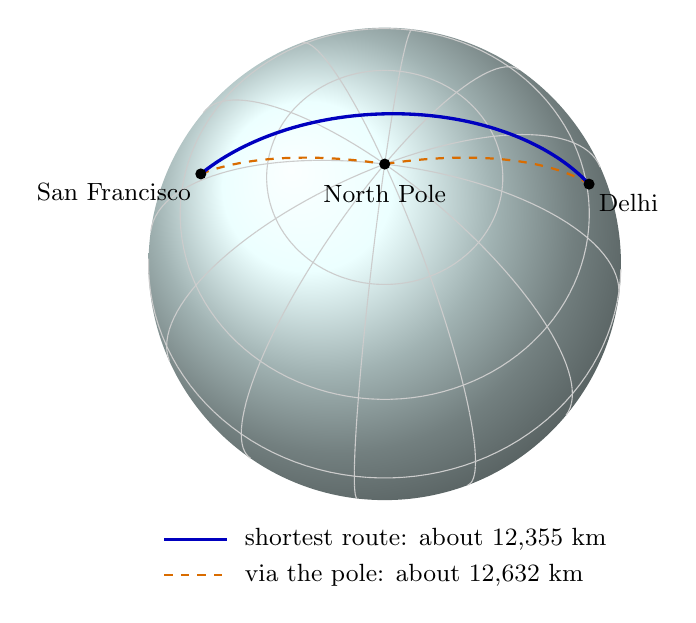
\begin{tikzpicture}[font=\small]
% Requires \usepackage{tikz}.
% View centred on 65 N, 22.6 W:
% San Francisco appears on the left, Delhi on the right.
\def\R{3}
\def\viewlat{65}
\def\viewlon{-22.6}

% Project latitude and longitude onto the drawing.
\pgfmathdeclarefunction{geoprojx}{2}{%
  \pgfmathparse{\R*cos(#1)*sin(#2-\viewlon)}}
\pgfmathdeclarefunction{geoprojy}{2}{%
  \pgfmathparse{\R*(sin(#1)*cos(\viewlat)
    -cos(#1)*cos(#2-\viewlon)*sin(\viewlat))}}
\pgfmathdeclarefunction{geodepth}{2}{%
  \pgfmathparse{sin(#1)*sin(\viewlat)
    +cos(#1)*cos(#2-\viewlon)*cos(\viewlat)}}

\shade[ball color=cyan!10] (0,0) circle (\R);

% Latitude circles: draw only the visible portions.
\foreach \lat in {-60,-30,0,30,60}{
  \foreach \lon in {-180,-177,...,177}{
    \pgfmathparse{geodepth(\lat,\lon+1.5)}
    \ifdim\pgfmathresult pt>0pt
      \draw[gray!40,thin]
        ({geoprojx(\lat,\lon)},{geoprojy(\lat,\lon)})
        -- ({geoprojx(\lat,\lon+3)},{geoprojy(\lat,\lon+3)});
    \fi
  }
}

% Meridians: draw only the visible portions.
\foreach \lon in {-180,-150,...,150}{
  \foreach \lat in {-90,-87,...,87}{
    \pgfmathparse{geodepth(\lat+1.5,\lon)}
    \ifdim\pgfmathresult pt>0pt
      \draw[gray!40,thin]
        ({geoprojx(\lat,\lon)},{geoprojy(\lat,\lon)})
        -- ({geoprojx(\lat+3,\lon)},{geoprojy(\lat+3,\lon)});
    \fi
  }
}

\coordinate (D) at
  ({geoprojx(28.6,77.2)},{geoprojy(28.6,77.2)});
\coordinate (S) at
  ({geoprojx(37.8,-122.4)},{geoprojy(37.8,-122.4)});
\coordinate (N) at
  ({geoprojx(90,0)},{geoprojy(90,0)});

% Longer route through the North Pole.
\draw[orange!85!black,thick,dashed]
  plot[domain=28.6:90,samples=70,variable=\t]
    ({geoprojx(\t,77.2)},{geoprojy(\t,77.2)});
\draw[orange!85!black,thick,dashed]
  plot[domain=37.8:90,samples=70,variable=\t]
    ({geoprojx(\t,-122.4)},{geoprojy(\t,-122.4)});

% Shorter great-circle arc, using spherical interpolation.
\pgfmathsetmacro{\angleDS}{
  acos(sin(28.6)*sin(37.8)
    +cos(28.6)*cos(37.8)*cos(77.2+122.4))}
\pgfmathsetmacro{\Dx}{geoprojx(28.6,77.2)}
\pgfmathsetmacro{\Dy}{geoprojy(28.6,77.2)}
\pgfmathsetmacro{\Sx}{geoprojx(37.8,-122.4)}
\pgfmathsetmacro{\Sy}{geoprojy(37.8,-122.4)}

\draw[blue!75!black,very thick]
  plot[domain=0:1,samples=120,variable=\t]
  ({(sin((1-\t)*\angleDS)*\Dx
       +sin(\t*\angleDS)*\Sx)/sin(\angleDS)},
   {(sin((1-\t)*\angleDS)*\Dy
       +sin(\t*\angleDS)*\Sy)/sin(\angleDS)});

\fill (S) circle (2pt) node[below left] {San Francisco};
\fill (D) circle (2pt) node[below right] {Delhi};
\fill (N) circle (2pt) node[below=4pt] {North Pole};

% Legend.
\draw[blue!75!black,very thick]
  (-2.8,-3.5)--(-2,-3.5);
\node[right] at (-1.9,-3.5)
  {shortest route: about 12,355 km};

\draw[orange!85!black,thick,dashed]
  (-2.8,-3.95)--(-2,-3.95);
\node[right] at (-1.9,-3.95)
  {via the pole: about 12,632 km};

\end{tikzpicture}
\caption{Delhi and San Francisco on a sphere, viewed from above
the northern Atlantic, with San Francisco to the left and Delhi
to the right. The blue great-circle arc reaches approximately
$75.6^\circ$N without passing through the North Pole.
The dashed orange route passes through the pole and is longer.
The grid marks latitude and longitude at $30^\circ$ intervals.
These are geometric routes, not records of actual flights.}
\label{fig:geo-delhi-sf-globe}
\end{figure}

The same great-circle route appears curved on the flat map in
Figure~\ref{fig:geo-delhi-sf}.

\begin{figure}[htbp]
\centering
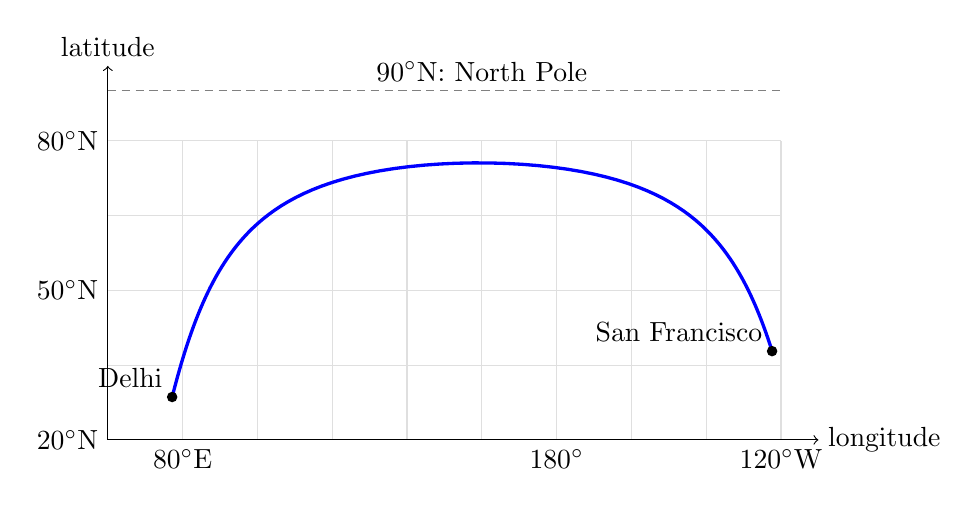
\begin{tikzpicture}[scale=0.95]
\draw[step=1,gray!25] (0,0) grid (9,4);
\draw[->] (0,0)--(9.5,0) node[right]{longitude};
\draw[->] (0,0)--(0,5) node[above]{latitude};
\foreach \y/\lab in {0/20,2/50,4/80} {\node[left] at (0,\y) {$\lab^\circ$N};}
\node[below] at (1,0) {$80^\circ$E};
\node[below] at (6,0) {$180^\circ$};
\node[below] at (9,0) {$120^\circ$W};
\draw[densely dashed,gray] (0,4.667)--(9,4.667);
\node[above] at (5,4.667) {$90^\circ$N: North Pole};
\draw[very thick,blue] plot coordinates {(0.8600,0.5733) (0.8782,0.6443) (0.8967,0.7152) (0.9157,0.7861) (0.9351,0.8569) (0.9550,0.9276) (0.9753,0.9982) (0.9963,1.0687) (1.0177,1.1391) (1.0398,1.2094) (1.0626,1.2796) (1.0860,1.3496) (1.1102,1.4196) (1.1351,1.4894) (1.1609,1.5590) (1.1876,1.6285) (1.2153,1.6978) (1.2440,1.7670) (1.2738,1.8359) (1.3048,1.9046) (1.3371,1.9731) (1.3708,2.0414) (1.4060,2.1093) (1.4428,2.1770) (1.4814,2.2444) (1.5218,2.3114) (1.5643,2.3780) (1.6091,2.4442) (1.6562,2.5100) (1.7059,2.5753) (1.7585,2.6400) (1.8143,2.7041) (1.8734,2.7676) (1.9362,2.8304) (2.0031,2.8923) (2.0745,2.9534) (2.1507,3.0135) (2.2322,3.0725) (2.3195,3.1302) (2.4132,3.1866) (2.5138,3.2414) (2.6220,3.2945) (2.7383,3.3457) (2.8634,3.3948) (2.9979,3.4414) (3.1424,3.4853) (3.2972,3.5261) (3.4628,3.5637) (3.6390,3.5975) (3.8258,3.6272) (4.0224,3.6525) (4.2279,3.6731) (4.4408,3.6885) (4.6592,3.6987) (4.8810,3.7033) (5.1035,3.7024) (5.3244,3.6960) (5.5413,3.6841) (5.7520,3.6670) (5.9548,3.6448) (6.1483,3.6181) (6.3317,3.5870) (6.5045,3.5519) (6.6666,3.5133) (6.8180,3.4714) (6.9592,3.4266) (7.0906,3.3792) (7.2128,3.3294) (7.3264,3.2776) (7.4321,3.2239) (7.5304,3.1685) (7.6220,3.1117) (7.7074,3.0535) (7.7871,2.9942) (7.8617,2.9338) (7.9316,2.8724) (7.9971,2.8102) (8.0587,2.7472) (8.1167,2.6835) (8.1714,2.6191) (8.2231,2.5542) (8.2719,2.4888) (8.3183,2.4229) (8.3622,2.3565) (8.4041,2.2897) (8.4439,2.2226) (8.4819,2.1552) (8.5181,2.0874) (8.5528,2.0193) (8.5861,1.9510) (8.6180,1.8824) (8.6486,1.8136) (8.6780,1.7446) (8.7064,1.6755) (8.7337,1.6061) (8.7602,1.5365) (8.7857,1.4668) (8.8104,1.3970) (8.8343,1.3270) (8.8575,1.2569) (8.8800,1.1867)};
\fill (0.86,0.5733) circle (2pt) node[above left]{Delhi};
\fill (8.88,1.1867) circle (2pt) node[above left]{San Francisco};
\end{tikzpicture}
\caption{The computed shorter great-circle arc on a latitude--longitude
map. Longitudes continue eastward across $180^\circ$. Equal distances on
this flat map do not represent equal distances on the Earth. This is a
geometric route, not a record of an actual flight.}
\label{fig:geo-delhi-sf}
\end{figure}

To find the distance, return to the idea used in Eratosthenes' measurement.
An arc occupies the same fraction of its circle's circumference as its
central angle occupies of a full turn. If the central angle is
$\alpha$ degrees, then
\[
 d=\frac{\alpha}{360^\circ}\,2\pi R.
\]
For these coordinates the central angle is approximately $111.1^\circ$.
Taking $R=6371$ km gives
\[
 d\approx\frac{111.1}{360}\times 2\pi\times6371
 \approx 12\,355\text{ km}.
\]
A route through the North Pole would instead cover
$(90-28.6)+(90-37.8)=113.6$ degrees along two meridians, or about
$12\,632$ km. Going exactly over the pole would therefore add about
$277$ km in this model.

\paragraph{Remark: calculating the central angle.}
Readers familiar with trigonometry can calculate it from latitudes
$\phi_1,\phi_2$ and the longitude difference $\Delta\lambda$:
\[
 \cos\alpha=\sin\phi_1\sin\phi_2+
 \cos\phi_1\cos\phi_2\cos(\Delta\lambda).
\]
Use the same angle units throughout. The formula supplies the angle;
the arc-length calculation then supplies the distance.

\paragraph{A geometric route and a flight route.}
The model explains why travelling far north can shorten the distance.
It does not determine the route of a particular flight. Winds, weather,
airspace restrictions, and operational requirements affect routing, and the
Earth is only approximately spherical. Thus the answer to our opening
question is: the shortest spherical route goes far north, but not exactly
over the pole; an actual flight need not follow that route exactly.


\section{Locating a point from distances}
\label{sec:geo-location}
\subsection{Coordinates turn a diagram into equations}
Choose perpendicular axes and a common unit. A point $P=(x,y)$ records
two signed displacements. By the Pythagorean theorem, the distance from
$P=(x,y)$ to $A=(a,b)$ is
\[
PA=\sqrt{(x-a)^2+(y-b)^2}.
\]
A negative coordinate is a direction, not a negative length. Coordinates
let us describe the same geometric relationships algebraically.

\begin{figure}[htbp]\centering
\begin{tikzpicture}[scale=.8]
\draw[->] (-.5,0)--(6,0) node[right]{$x$};\draw[->] (0,-.5)--(0,4.6) node[above]{$y$};
\coordinate (A) at (1,1);\coordinate (P) at (5,4);\coordinate (R) at (5,1);
\draw[thick,blue!65!black] (A)--node[above,sloped]{$PA$}(P);
\draw[dashed] (A)--node[below]{$x-a$}(R)--node[right]{$y-b$}(P);
\draw (4.75,1)--(4.75,1.25)--(5,1.25);
\fill (A) circle(2pt) node[left]{$A=(a,b)$};\fill (P) circle(2pt) node[above]{$P=(x,y)$};
\end{tikzpicture}
\caption{For the configuration drawn, the horizontal and vertical lengths are $x-a$ and $y-b$. In general use their absolute values; squaring removes the signs.}
\end{figure}

\subsection{One circle, two circles, three measurements}
Knowing that a point is five units from $A$ confines it to a circle;
it does not tell us which point on that circle it is. A second distance
usually leaves two possibilities. A third suitably placed landmark can
distinguish them.

\paragraph{The problem.}
Given $A=(0,0)$ and $B=(6,0)$, find all points $P$ with $PA=PB=5$.
Determine whether one additional exact distance from $C=(3,6)$
distinguishes those points. All distances are Euclidean.

If $P=(x,y)$ and $PA=PB=5$, then
\[
x^2+y^2=25,\qquad(x-6)^2+y^2=25.
\]
Subtracting the equations gives $12x-36=0$, so $x=3$. Substitution gives
$y^2=16$, leaving $P=(3,4)$ or $P=(3,-4)$.
A third landmark $C=(3,6)$ distinguishes them: their distances from $C$
are $2$ and $10$, respectively.

\begin{figure}[htbp]\centering
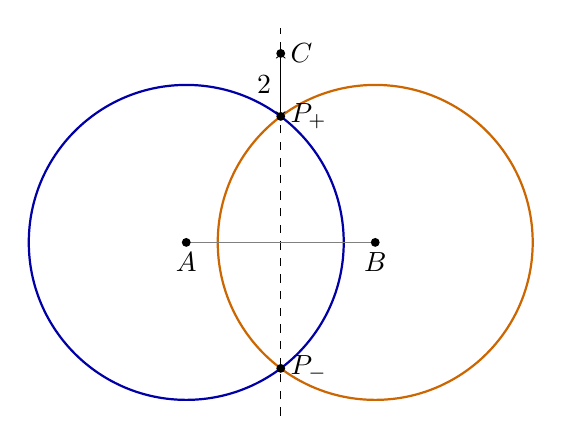
\begin{tikzpicture}[scale=.4]
\draw[blue!65!black,thick] (0,0) circle(5);\draw[orange!80!black,thick] (6,0) circle(5);
\draw[dashed] (3,-5.5)--(3,6.8);\draw[gray] (0,0)--(6,0);
\foreach \x/\y/\lab/\pos in {0/0/A/below,6/0/B/below,3/4/P_+/right,3/-4/P_-/right,3/6/C/right}{\fill (\x,\y) circle(4pt) node[\pos]{$\lab$};}
\draw[<->] (3,4)--node[left]{$2$}(3,6);
\end{tikzpicture}
\caption{Two distances leave a reflection ambiguity. A landmark off the baseline can distinguish the two points.}
\end{figure}

Two circles can also be tangent, disjoint, or coincident. With measured
rather than exact distances, three circles may have no common point.
This can indicate measurement error rather than a failure of geometry.
Each uncertain distance is better represented by a thin ring; plausible
locations lie in the overlap of the rings.

\begin{figure}[htbp]\centering
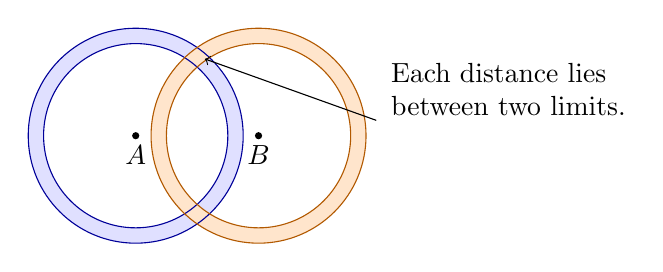
\begin{tikzpicture}[scale=.65]
\fill[blue!12,even odd rule] (0,0) circle(2.1) (0,0) circle(1.8);
\fill[orange!20,even odd rule] (2.4,0) circle(2.1) (2.4,0) circle(1.8);
\draw[blue!60!black] (0,0) circle(2.1) (0,0) circle(1.8);
\draw[orange!70!black] (2.4,0) circle(2.1) (2.4,0) circle(1.8);
\fill (0,0) circle(2pt) node[below]{$A$};\fill (2.4,0) circle(2pt) node[below]{$B$};
\node[right,align=left] at (4.8,.9) {Each distance lies\\between two limits.};
\draw[->] (4.7,.3)--(1.35,1.5);
\end{tikzpicture}
\caption{Uncertain measurements give regions of possible locations, often with more than one separate component.}
\end{figure}

\subsection{Which clinic is nearest?}
\begin{figure}[htbp]\centering
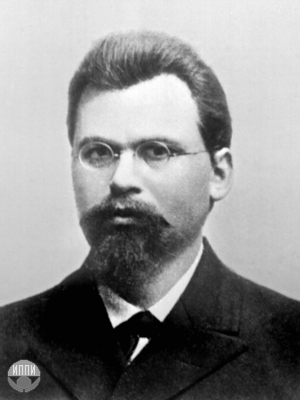
\includegraphics[height=1.4in]{images/voronoi.jpg}
\caption{Georgy Voronoi (1868--1908), whose name is attached to these
nearest-site regions. Photograph, photographer unknown;
\href{https://commons.wikimedia.org/wiki/File:Georgy_Voronoy.jpg}{Wikimedia Commons, marked public domain}.}
\label{fig:geo-voronoi-portrait}
\end{figure}
\paragraph{The problem.}
Given finitely many distinct clinic locations in the Euclidean plane,
describe, for each clinic, every point at least as close to it as to any
other clinic. Include ties on shared boundaries. Assume straight-line
travel is possible and all clinics are equally suitable.

Suppose two clinics are at $A=(-2,0)$ and $B=(2,0)$. For $P=(x,y)$,
\[
PA^2-PB^2=(x+2)^2+y^2-\bigl((x-2)^2+y^2\bigr)=8x.
\]
Thus $P$ is nearer $A$ when $x<0$, nearer $B$ when $x>0$, and equally
far from both when $x=0$. The boundary is the perpendicular bisector
of $AB$. Translating or rotating the picture does not change the result.

For several clinics, the region belonging to $A$ consists of all points
at least as near to $A$ as to every other clinic. For each competitor,
keep the half-plane containing $A$ bounded by their perpendicular bisector.
The intersection of those half-planes is $A$'s \emph{Voronoi region}.\footnote{The regions are named after Georgy Voronoi (also written Voronoy, 1868--1908).
For further examples and applications, see
\href{https://en.wikipedia.org/wiki/Voronoi_diagram}{Wikipedia, ``Voronoi diagram.''}}
Boundary points may belong to more than one region because of ties.

\begin{figure}[htbp]\centering
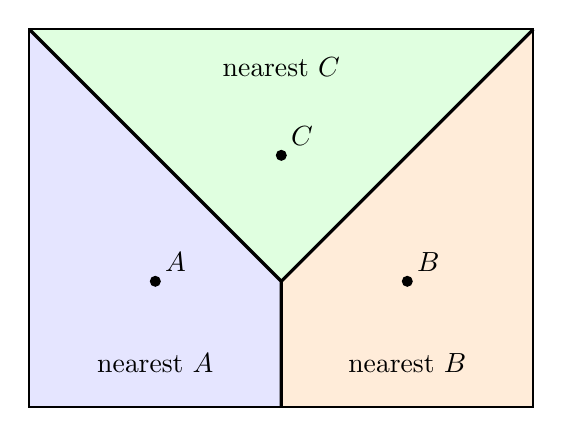
\begin{tikzpicture}[scale=.8]
\fill[blue!10] (-4,-2)--(0,-2)--(0,0)--(-4,4)--cycle;
\fill[orange!15] (0,-2)--(4,-2)--(4,4)--(0,0)--cycle;
\fill[green!12] (-4,4)--(0,0)--(4,4)--(4,4)--(-4,4)--cycle;
\draw[thick] (-4,-2) rectangle (4,4);
\draw[very thick] (0,-2)--(0,0)--(-4,4);\draw[very thick] (0,0)--(4,4);
\foreach \x/\y/\lab in {-2/0/A,2/0/B,0/2/C}{\fill (\x,\y) circle(2.5pt) node[above right]{$\lab$};}
\node at (-2,-1.3) {nearest $A$};\node at (2,-1.3) {nearest $B$};\node at (0,3.4) {nearest $C$};
\end{tikzpicture}
\caption{Three nearest-clinic regions, clipped to a rectangular map. Here $A=(-2,0)$, $B=(2,0)$, and $C=(0,2)$; the three boundaries meet at $(0,0)$.}
\label{fig:geo-voronoi}
\end{figure}

A region is not necessarily bounded: a clinic near the edge of the set of
sites can have a region extending indefinitely. The border of a printed
map is not a nearest-distance boundary. Nor does ``nearest'' automatically
mean ``best served'': travel time, capacity, and barriers may matter more.

\subsection{Changing the meaning of distance}
\paragraph{The problem.}
Given two grid intersections $P=(x_P,y_P)$ and $Q=(x_Q,y_Q)$ with integer
coordinates, determine the shortest route length using unit horizontal
or vertical street segments. Every segment is available and has unit cost.

On an ideal rectangular street grid, suppose we can move only horizontally
and vertically and every street is available. The shortest route length is
\[
d_{\rm grid}(P,Q)=|x_P-x_Q|+|y_P-y_Q|.
\]
Every route must cover at least those horizontal and vertical displacements;
a route that never reverses direction attains their sum. This proves the
formula. Between $(0,0)$ and $(3,2)$ it gives $5$, whereas straight-line
distance gives $\sqrt{13}$. The nearest-clinic boundaries can change when
the distance model changes.

\begin{figure}[htbp]\centering
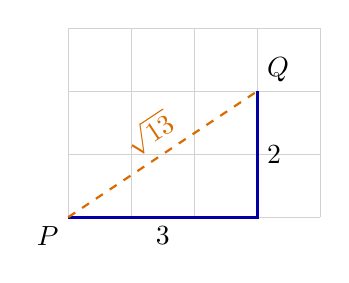
\begin{tikzpicture}[scale=.8]
\draw[step=1,gray!35] (0,0) grid (4,3);
\draw[very thick,blue!65!black] (0,0)--(3,0)--(3,2);
\draw[thick,dashed,orange!85!black] (0,0)--node[above,sloped]{$\sqrt{13}$}(3,2);
\node[below left] at (0,0) {$P$};\node[above right] at (3,2) {$Q$};
\node[below] at (1.5,0) {$3$};\node[right] at (3,1) {$2$};
\end{tikzpicture}
\caption{The straight route is shorter, but the street model does not permit it. A shortest admissible route has length $5$.}
\end{figure}

\section{Finding a shortest route}
\label{sec:geo-shortest}
\subsection{A route that must touch a straight boundary}
\paragraph{The problem.}
Let $A$ and $B$ lie strictly on the same side of a straight boundary $\ell$.
We want a route from $A$ to $B$ that touches $\ell$, perhaps to collect
water along a straight stretch of riverbank. Assuming open terrain and
equal cost per unit length, choose $X$ on $\ell$ to minimise $AX+XB$.

Reflect $B$ across $\ell$ to obtain $B'$. Every point $X$ of $\ell$
satisfies $XB=XB'$, so
\[
AX+XB=AX+XB'\geq AB'.
\]
The inequality is the triangle inequality. Equality holds when $X$ is
where the straight segment $AB'$ crosses $\ell$. Because $A$ and $B'$
are on opposite sides, that intersection exists. The lower bound is
attained, which proves that the constructed route is shortest.

\begin{figure}[htbp]\centering
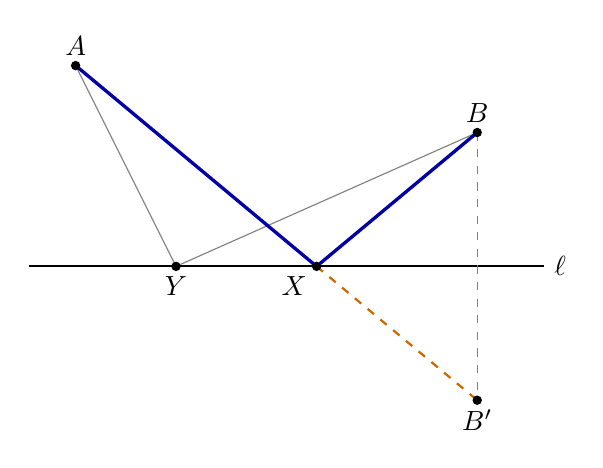
\begin{tikzpicture}[scale=.85]
\coordinate (A) at (0,3);\coordinate (B) at (6,2);\coordinate (Bp) at (6,-2);\coordinate (X) at (3.6,0);\coordinate (Y) at (1.5,0);
\draw[thick] (-.7,0)--(7,0) node[right]{$\ell$};
\draw[gray,dashed] (B)--(Bp);\draw[gray] (A)--(Y)--(B);
\draw[very thick,blue!65!black] (A)--(X)--(B);
\draw[thick,dashed,orange!80!black] (X)--(Bp);
\foreach \p/\lab/\pos in {A/A/above,B/B/above,Bp/B'/below,X/X/below left,Y/Y/below}{\fill (\p) circle(2pt) node[\pos]{$\lab$};}
\end{tikzpicture}
\caption{Reflect the destination. The best broken route becomes a straight segment; a different touching point $Y$ gives a longer route.}
\end{figure}

\paragraph{From the proof to a procedure.}
Construct the perpendicular from $B$ to $\ell$ and extend it by the same
length on the other side to obtain $B'$. Draw $AB'$ and mark its intersection
$X$ with $\ell$. Follow $AX$ and then $XB$. The proof supplies both the
construction and the certificate that no other touching point is better.

For $A=(0,3)$, $B=(6,2)$, and $\ell$ the horizontal axis, $B'=(6,-2)$.
The straight segment drops five units in six horizontal units, and reaches
the axis after a drop of three, so $X=(18/5,0)$. The shortest length is
$AB'=\sqrt{61}$. If only a finite stretch of bank is accessible, first
check that $X$ belongs to it; the construction for an unrestricted line
need not solve the constrained problem.

\subsection{Unfolding a surface}
A route drawn straight through a box is not a route along its surface.
But unfolding adjacent flat faces preserves lengths within those faces.
A shortest route crossing a specified shared edge can therefore be found
by laying the faces flat and drawing a straight segment, provided that
segment stays within the unfolded faces and crosses the intended edge.

\paragraph{The problem.}
For a rectangular box with edge lengths $a=4$, $b=3$, $c=2$ and opposite
corners $P,Q$, compare the three two-face routes obtained by unfolding
rectangles of dimensions $(a+b)\times c$, $(a+c)\times b$, and
$(b+c)\times a$. Check that each straight segment stays on those faces,
and find the shortest of these candidates. Lengths use a common unit.

The three unfoldings give the candidate lengths
\[
\sqrt{(a+b)^2+c^2}=\sqrt{53},\quad
\sqrt{(a+c)^2+b^2}=\sqrt{45},\quad
\sqrt{(b+c)^2+a^2}=\sqrt{41}.
\]
These are lengths of admissible surface routes, not of the space diagonal.
The third is the shortest of these candidates. Comparing candidates is a
useful step, but a claim of global optimality also needs a proof that
no other face sequence does better; we do not assume that merely from a drawing.

\begin{figure}[htbp]\centering
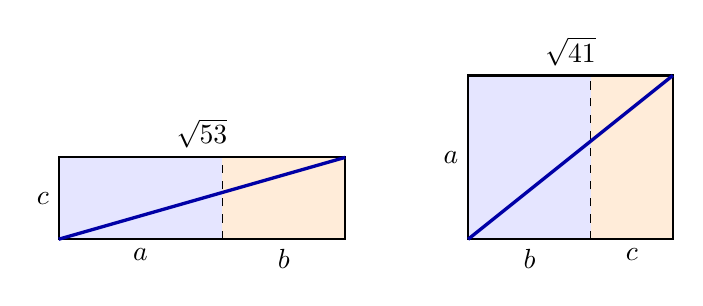
\begin{tikzpicture}[scale=.52]
\begin{scope}
\fill[blue!10] (0,0) rectangle (4,2);\fill[orange!15] (4,0) rectangle (7,2);
\draw[thick] (0,0) rectangle (7,2);\draw[dashed] (4,0)--(4,2);\draw[very thick,blue!65!black] (0,0)--(7,2);
\node[below] at (2,0) {$a$};\node[below] at (5.5,0) {$b$};\node[left] at (0,1) {$c$};
\node[above] at (3.5,2) {$\sqrt{53}$};
\end{scope}
\begin{scope}[xshift=10cm]
\fill[blue!10] (0,0) rectangle (3,4);\fill[orange!15] (3,0) rectangle (5,4);
\draw[thick] (0,0) rectangle (5,4);\draw[dashed] (3,0)--(3,4);\draw[very thick,blue!65!black] (0,0)--(5,4);
\node[below] at (1.5,0) {$b$};\node[below] at (4,0) {$c$};\node[left] at (0,2) {$a$};\node[above] at (2.5,4) {$\sqrt{41}$};
\end{scope}
\end{tikzpicture}
\caption{Two of the three candidate unfoldings. Dashed lines are folds, not barriers. The endpoints of each diagonal represent opposite corners of the box.}
\end{figure}

\paragraph{Try it with paper.}
Make a $4\times3\times2$ box, mark opposite corners, and transfer the
shorter route from its unfolding back onto the box. It will bend in space
at the fold although it was straight on the paper. The relevant geometry
is that of the permitted surface.

\section{Shape, size, and efficiency}
\label{sec:geo-efficiency}
\subsection{The largest rectangular garden}
\paragraph{The problem.}
Suppose a rectangular garden has a fixed perimeter $P>0$, with all four
sides fenced. If its side lengths are $x,y>0$, then $x+y=P/2$.
We want to maximise its area $xy$.

The identity
\[
(x+y)^2-(x-y)^2=4xy
\]
gives
\[
xy=\frac{P^2}{16}-\frac{(x-y)^2}{4}\leq\frac{P^2}{16}.
\]
Equality holds exactly when $x=y=P/4$. Thus the square has the greatest
area \emph{among rectangles with that perimeter}. The restriction to
rectangles is part of the claim. We have both an upper bound and a shape
that attains it, just as the reflection argument gave a lower bound and
a route attaining it.

\begin{figure}[htbp]\centering
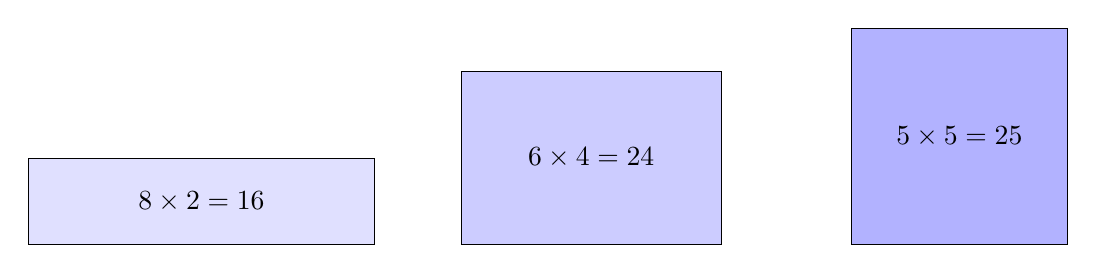
\begin{tikzpicture}[scale=.55]
\filldraw[fill=blue!12] (0,0) rectangle (8,2);\node at (4,1) {$8\times2=16$};
\filldraw[fill=blue!20] (10,0) rectangle (16,4);\node at (13,2) {$6\times4=24$};
\begin{scope}[xshift=19cm]\filldraw[fill=blue!30] (0,0) rectangle (5,5);\node at (2.5,2.5) {$5\times5=25$};\end{scope}
\end{tikzpicture}
\caption{Each rectangle has perimeter $20$. Equalising the side lengths increases area.}
\end{figure}

\paragraph{A changed problem.}
Now an existing straight wall can supply one entire side at no fencing
cost. It is long enough for any proposed garden. With the same available
fencing length $P$, determine the largest rectangular area and its dimensions.

The constraint changes to $2x+y=P$, where
$x$ measures distance away from the wall. Then
\[
xy=x(P-2x)=\frac{P^2}{8}-2\left(x-\frac P4\right)^2.
\]
The optimum now has $x=P/4$ and $y=P/2$: it is not a square.
A correct answer belongs to a specified problem, not just to a familiar picture.

\subsection{Enlarging a shape}
\paragraph{The problem.}
A plane figure or solid is enlarged uniformly by a factor $k>0$ in every
linear dimension. Determine the factors by which its area or volume
changes. For a solid, also determine the change in surface-area-to-volume ratio.

If every length of a shape is multiplied by $k>0$, corresponding areas
are multiplied by $k^2$ and volumes by $k^3$. For a rectangle this follows
from $(kx)(ky)=k^2xy$; for a rectangular box it follows from
$(kx)(ky)(kz)=k^3xyz$. Decomposing a polygon into triangles gives the
same area rule, and the volume rule extends to similar solids.

\begin{figure}[htbp]\centering
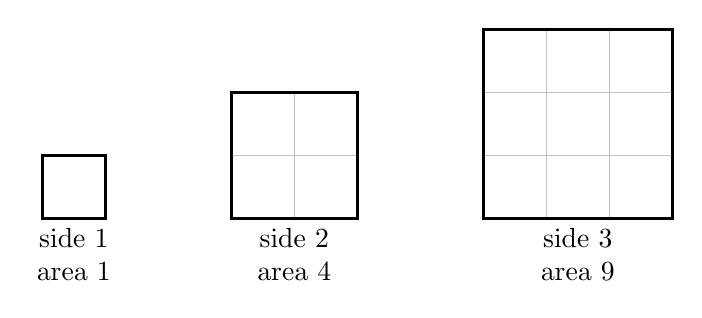
\begin{tikzpicture}[scale=.8]
\draw[step=1,gray!50] (0,0) grid (1,1);\draw[very thick] (0,0) rectangle (1,1);\node[below,align=center] at (.5,0) {side $1$\\area $1$};
\draw[step=1,gray!50] (3,0) grid (5,2);\draw[very thick] (3,0) rectangle (5,2);\node[below,align=center] at (4,0) {side $2$\\area $4$};
\draw[step=1,gray!50] (7,0) grid (10,3);\draw[very thick] (7,0) rectangle (10,3);\node[below,align=center] at (8.5,0) {side $3$\\area $9$};
\end{tikzpicture}
\caption{Scaling every length by $k$ requires $k^2$ unit squares to cover the enlarged square when $k$ is an integer. The algebraic rule also holds for noninteger $k>0$.}
\end{figure}

Doubling a box's dimensions therefore requires four times as much surface
material but gives eight times the capacity, if thickness is neglected.
The surface-area-to-volume ratio is divided by two. These statements
compare \emph{similar} boxes; changing only one dimension is a different
operation.

\subsection{Cutting a cube into pieces}
\paragraph{The problem.}
A cube of side $s>0$ is cut by planes parallel to its faces into equal
cubes, with $m\geq1$ divisions along each edge. Neglect the thickness of
cuts. Determine the number of pieces, their total volume and total surface
area, and the newly exposed area when all pieces are separated.

Take a cube of side $s$, and divide each edge into $m$ equal parts, where
$m\geq1$ is an integer. There are $m^3$ small cubes, each of side $s/m$.
Their combined volume is
\[
m^3(s/m)^3=s^3,
\]
but the sum of all their surface areas is
\[
m^3\,6(s/m)^2=6ms^2.
\]
That is $m$ times the surface area of the original cube. The extra area
comes from newly exposed cut faces, not from extra volume. If the pieces
remain pressed together, those internal faces are not exposed to the surroundings.

\begin{figure}[htbp]\centering
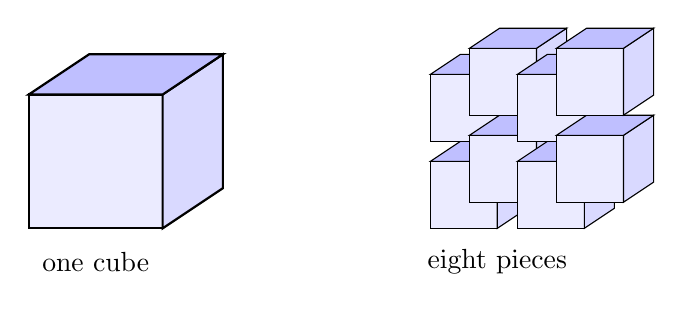
\begin{tikzpicture}[x={(1cm,0cm)},y={(.45cm,.3cm)},z={(0cm,1cm)},scale=.85]
\draw[thick,fill=blue!8] (0,0,0)--(2,0,0)--(2,0,2)--(0,0,2)--cycle;
\draw[thick,fill=blue!15] (2,0,0)--(2,2,0)--(2,2,2)--(2,0,2)--cycle;
\draw[thick,fill=blue!25] (0,0,2)--(2,0,2)--(2,2,2)--(0,2,2)--cycle;
\node at (1,0,-.5) {one cube};
\begin{scope}[xshift=6cm]
\foreach \a in {0,1}{\foreach \b in {0,1}{\foreach \c in {0,1}{
\begin{scope}[shift={(1.3*\a,1.3*\b,1.3*\c)}]
\draw[fill=blue!8] (0,0,0)--(1,0,0)--(1,0,1)--(0,0,1)--cycle;
\draw[fill=blue!15] (1,0,0)--(1,1,0)--(1,1,1)--(1,0,1)--cycle;
\draw[fill=blue!25] (0,0,1)--(1,0,1)--(1,1,1)--(0,1,1)--cycle;
\end{scope}}}}
\node at (1,0,-.5) {eight pieces};
\end{scope}
\end{tikzpicture}
\caption{For $m=2$, volume is unchanged but the total surface area of the separated pieces doubles. The gaps illustrate separation and are not part of the original cube.}
\end{figure}

This helps explain why crushing or cutting a material can make surface
processes faster. Geometry identifies the changed area; a prediction of
the actual rate also needs a model of the physical process.

\subsection{Packaging: state what is being optimised}
\paragraph{The problem.}
Among all closed boxes with a square base and prescribed volume $V>0$,
find dimensions that minimise total surface area, and prove the minimum.
The dimensions may be any positive real numbers; ignore material thickness,
seams, and waste in cutting.

Consider a closed box with square base of side $x$ and height $h$,
required to contain $V$ cubic units. Ignoring thickness and seams,
\[
x^2h=V,\qquad S=2x^2+4xh=2x^2+\frac{4V}{x}.
\]
For $V=1000$, the boxes $(x,h)=(5,40),(10,10),(20,2.5)$ have surface
areas $850,600,1000$, respectively. A table suggests a good design, but
three trials do not prove optimality.

Here a proof is possible without calculus. Put $s=\sqrt[3]{V}$ and
$t=x/s>0$. Then
\[
\frac{S}{2s^2}-3=t^2+\frac2t-3
=\frac{(t-1)^2(t+2)}t\geq0.
\]
Thus $S\geq6V^{2/3}$, with equality exactly at $t=1$: the cube is best
within this family of closed boxes. An open box has only one base, and
extra conditions such as shelf height, openings, seams, or strength change
the problem. The model tells us what our optimisation does and does not establish.

\section{A bridge back to algorithms: area from vertices}
\label{sec:geo-polygon}
\paragraph{The problem.}
Given the coordinates of the $n\geq3$ vertices of a simple polygon in
boundary order, compute its area. Give a procedure whose arithmetic-operation
count grows linearly with $n$. The input boundary does not cross itself;
clockwise and anticlockwise orders must both be accepted.

A survey may give the vertices of a field rather than its area. Suppose
$P_i=(x_i,y_i)$, $i=1,\ldots,n$, list the vertices of a simple polygon
in order around its boundary. ``Simple'' means that its edges do not cross.
Set $P_{n+1}=P_1$. Its area is
\[
A=\frac12\left|\sum_{i=1}^{n}
(x_i y_{i+1}-x_{i+1}y_i)\right|.
\]
This is the \emph{shoelace formula}. The order of the vertices is essential;
sorting them arbitrarily by one coordinate can describe a different boundary.

\begin{figure}[htbp]\centering
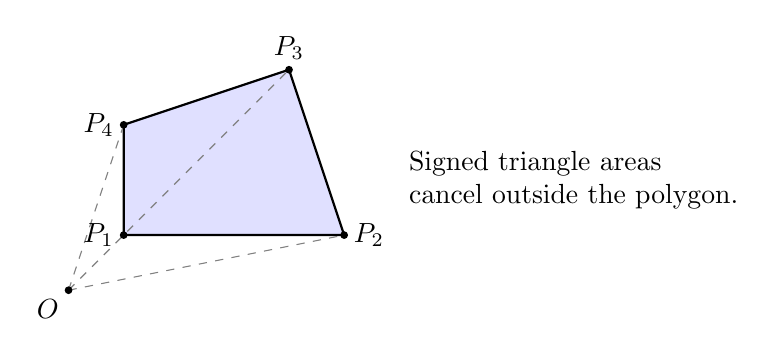
\begin{tikzpicture}[scale=.7]
\coordinate (O) at (0,0);\coordinate (A) at (1,1);\coordinate (B) at (5,1);\coordinate (C) at (4,4);\coordinate (D) at (1,3);
\fill[blue!12] (A)--(B)--(C)--(D)--cycle;
\draw[thick] (A)--(B)--(C)--(D)--cycle;
\draw[dashed,gray] (O)--(A) (O)--(B) (O)--(C) (O)--(D);
\foreach \p/\lab/\pos in {O/O/below left,A/P_1/left,B/P_2/right,C/P_3/above,D/P_4/left}{\fill (\p) circle(2pt) node[\pos]{$\lab$};}
\node[right,align=left] at (6,2) {Signed triangle areas\\cancel outside the polygon.};
\end{tikzpicture}
\caption{Summing oriented triangles from an origin gives the polygon area, even when that origin is outside.}
\end{figure}

Why does this work? The signed area of the triangle $OP_iP_{i+1}$ is
$\tfrac12(x_i y_{i+1}-x_{i+1}y_i)$, positive for an anticlockwise turn
and negative for a clockwise turn. The formula follows by subtracting
right-triangle areas, or by taking base times perpendicular height.
Triangulate the polygon, and orient each triangle anticlockwise. In the
sum of their coordinate expressions, every internal edge occurs in both
directions and cancels. Only the boundary terms remain. Reversing the
boundary order changes the sign; the absolute value recovers ordinary area.

For $(0,0),(4,0),(4,3),(0,3)$ the sum is $24$, giving area $12$.
For the quadrilateral in the figure the sum is $18$, giving area $9$.
A self-crossing boundary needs separate interpretation: signed regions
can cancel, so the formula need not give the total area one intended.

The desired loop postcondition is that an accumulator $z$ contains all
$n$ terms. Generalise ``all'' to ``the first $k$'':
\[
0\leq k\leq n,\qquad
z=\sum_{i=1}^{k}(x_i y_{i+1}-x_{i+1}y_i).
\]
Begin with $k=0,z=0$. While $k<n$, add the term with index $k+1$ to $z$,
then increment $k$. The displayed assertion is preserved, and the bound
function $n-k$ decreases by one. Return $|z|/2$. This connects a geometric
proof directly to an iterative procedure requiring $O(n)$ arithmetic operations.

\section{What a geometric answer should contain}
We have repeatedly followed the same route: state the question, draw a
model, identify assumptions, prove a relationship, and turn it into a
calculation or construction. Finally, interpret the result in the original
setting. A number without units, a diagram without justified relationships,
or an optimum without a specified constraint is only part of an answer.

Geometry also gives us ways to check our work. Does the formula have the
right units? Does it behave sensibly when a length doubles? Does an equality
case attain the bound? Does the constructed route stay in the permitted
region? These questions connect visual understanding to mathematical proof.

\section*{Problems}
Unless stated otherwise, coordinates refer to a Euclidean plane with a
common unit on both axes. Draw labelled diagrams where helpful. For
measurement problems, distinguish the conclusion within the stated model
from possible errors in the model itself.
\begin{enumerate}
\setlength{\itemsep}{0pt}
\setlength{\parsep}{0pt}
\item \textbf{Height from shadows.} A vertical stick of height $1.2$ metres
casts a shadow of length $0.8$ metres, while a vertical tree casts a shadow
of length $7$ metres at the same instant. Assume level ground and parallel
sunlight. Estimate the tree's height using similarity, and identify two
physical departures from the assumptions that would invalidate the estimate.

\item \textbf{Bounds on the height.} In the preceding shadow model, take
the stick height to be exactly $1.2$ metres, its shadow length to lie in
$[0.75,0.85]$ metres, and the tree's shadow length in $[6.8,7.2]$ metres.
Find the smallest interval containing every tree height allowed by these
bounds, with no further relationship assumed between the measurement errors.
Give exact endpoints and an outward-rounded interval to two decimal places.

\item \textbf{An unequal-baseline river construction.} Points $A,B,C$
lie in that order on a straight baseline, with $AB=12$ and $BC=8$ metres.
The segments $AT$ and $CD$ are perpendicular to the baseline on opposite
sides, $T,B,D$ are collinear, and $CD=10$ metres. Determine $AT$ by
similarity. Derive the general relation between $AT,AB,BC,CD$ and explain
what simplifies when $AB=BC$.

\item \textbf{Design a field measurement.} Choose one inaccessible height
or distance on campus, and define precisely its endpoints. Propose a
procedure using a tape, a vertical stick, and sight lines (you need not
perform it). Supply a labelled diagram, a list of accessible measurements,
the assumptions and formula used to infer the desired length, and one
repeat measurement that would help detect an error. Explain what that
repeat measurement checks.

\item \textbf{Locating a point.} Let $A=(0,0)$ and
$B=(8,0)$. Find all points $P$ satisfying $PA=PB=5$. Give coordinates for a third landmark whose distance to $P$
distinguishes the possible points, and for a different landmark whose
distance does not. Compute the relevant distances to justify both choices.

\item \textbf{How many circle intersections?} Two circles have radii
$r_1,r_2>0$ and distinct centres at distance $d>0$. Give necessary and
sufficient conditions, in terms of $r_1,r_2,d$, for zero, one, and two
intersection points. Distinguish external tangency from internal tangency,
and disjoint circles lying outside one another from one lying inside the other.
Illustrate each case.

\item \textbf{Three Voronoi regions.} The only sites are $A=(0,0)$,
$B=(6,0)$, and $C=(0,6)$. For each site, derive inequalities defining the
points at least as close to it as to both others. Draw all three regions
in the whole plane, mark the parts of the bisectors where nearest-site ties
occur, and identify the point tied among all three sites.

\item \textbf{Straight-line distance versus road distance.} Construct a
connected road network containing a home $H$ and two clinics $A,B$, with
$HA<HB$ in Euclidean distance but with the shortest road route from $H$
to $A$ longer than that from $H$ to $B$. Give coordinates for every junction,
list all roads and their lengths, and calculate both shortest road distances.
Use straight road segments with lengths given by their coordinates; travel
is allowed only along the listed roads.

\item \textbf{Counting shortest grid routes.} In the unobstructed integer
square grid, every horizontal or vertical edge has length one and may be
traversed in either direction. Find the shortest length from $(0,0)$ to
$(3,2)$ and count all routes attaining it. Explain why no shortest route
can include a westward or southward step.

\item \textbf{A route touching a boundary.} Let $A=(0,2)$ and $B=(8,4)$.
Among all broken straight routes $A\!\to X\!\to B$ with $X=(t,0)$,
$t\in\mathbb R$, find the minimising point $X$ and the minimum length.
Prove optimality by reflection. Repeat with the additional constraint
$0\leq t\leq1$, giving a proof that your constrained minimiser is best.

\item \textbf{Equal angles at the boundary.} Let $A,B$ lie strictly on
the same side of a line $\ell$, and let $X\in\ell$ minimise $AX+XB$.
Prove that the smaller angle between $AX$ and $\ell$ equals the smaller
angle between $BX$ and $\ell$. Include the case in which both segments
are perpendicular to $\ell$, and identify where reflection is used.

\item \textbf{Routes on a box.} A rectangular box has edge lengths
$5,4,1$ units. Join opposite corners by the three two-face routes obtained
from unfolded rectangles $(5+4)\times1$, $(5+1)\times4$, and
$(4+1)\times5$. Draw each unfolding with its fold and endpoints, find the
three lengths, and identify the smallest. Check that each diagonal crosses
the intended shared edge within that edge. Compare only these candidates;
a proof about all possible face sequences is not required.

\item \textbf{Fencing a garden.} Exactly $40$ metres of fencing is
available for a rectangular garden with positive side lengths. Find the
maximum area and the dimensions attaining it (a) when all four sides must
be fenced and (b) when an existing straight wall supplies one side. In (b)
assume the wall is long enough and the remaining three sides use all the
fencing. Prove both maxima algebraically.

\item \textbf{A scale model.} A model building is geometrically similar
to the actual building, with every model length equal to $1/50$ of the
corresponding actual length. Find the ratios model:actual for corresponding
areas and volumes. If $A$ square centimetres of model surface requires
painting, express the corresponding actual area in square centimetres and
explain why multiplying $A$ by $50$ is incorrect.

\item \textbf{Cutting a cube.} A solid cube of side $12$ cm is cut into
cubes of side $3$ cm by planes parallel to its faces. Neglect material lost
in cutting. Find the number of pieces, their combined volume, and the sum
of their surface areas. After every piece is separated, how much exposed
area is additional to the original cube's surface area? Include units.

\item \textbf{A closed box.} A closed box has a square base of side
$x>0$ cm, height $h>0$ cm, and volume $216$ cubic centimetres. Neglect
thickness and seams. Find the least possible total surface area, prove
that no admissible box has a smaller area, and identify all dimensions
attaining the minimum. Do not use calculus.

\item \textbf{An open box.} An open-top box has a square base of side
$x>0$ and prescribed volume $V>0$. Its height is $h=V/x^2$ and its
material area is $S=x^2+4V/x$. Prove without calculus that the unique
minimum occurs at $x^3=2V$, give the minimum area in terms of $V$, and
show that the optimal height is $x/2$. You may adapt the nonnegative
factorisation used for the closed box.

\item \textbf{Area from coordinates.} A polygon has vertices
$(0,0),(5,0),(5,2),(2,4),(0,2)$ in the listed boundary order, with the last
vertex joined to the first. Calculate its area using the shoelace formula.
Verify it independently by decomposing the polygon into a rectangle and
a triangle. Give the area in square coordinate units.

\item \textbf{Translation and the shoelace sum.} Let
$P_i=(x_i,y_i)$, $1\leq i\leq n$, be a closed polygonal sequence with
$P_{n+1}=P_1$. For fixed real numbers $a,b$, replace every vertex by
$(x_i+a,y_i+b)$. Prove that the signed sum
$\sum_{i=1}^n(x_i y_{i+1}-x_{i+1}y_i)$ is unchanged by expanding the
translated sum and cancelling terms. Deduce area invariance for a simple polygon.

\item \textbf{A crossed boundary.} Join $(0,0),(2,2),(0,2),(2,0)$ in
that order and close the boundary. Draw the resulting crossed figure.
Compute both the signed shoelace sum and half its absolute value. Separately
find the sum of the ordinary areas of its two triangular lobes. Explain
why these results differ and which hypothesis of the polygon-area formula fails.

\item \textbf{Earth's circumference from latitude.} Model Earth as a
sphere. Two sites on the same meridian have latitudes $18^\circ$ N and
$25.5^\circ$ N, and their meridian arc separation is $825$ km. Estimate
the great-circle circumference. If the sites have different longitudes,
explain why their latitude difference cannot simply be substituted for
the angle between their radii in the same calculation.

\item \textbf{An angle does not fix a size.} Fix an angle
$0<\theta<180^\circ$. Draw two circles of different radii, each with two
radii enclosing $\theta$. Explain why the same shadow-angle observation
could be consistent with either sphere. Identify one additional length
measurement that would determine the circumference and give the formula.

\item \textbf{Uncertainty in Earth's circumference.} In a spherical
model, two sites on one meridian have separation $d\in[595,605]$ km and
central angle $\theta\in[5.3^\circ,5.5^\circ]$. Assume no further relation
between these uncertainties. Find the smallest interval containing every
value of $C=360^\circ d/\theta$ consistent with the bounds. State which
endpoints determine each extreme and give an outward-rounded interval in
whole kilometres.

\item \textbf{Choosing a baseline.} Assume a spherical Earth of
circumference $40{,}000$ km. Compare meridian baselines of $100$ km and
$800$ km. Calculate their true central angles. For each, suppose the
reported angle equals that true angle but has uncertainty $\pm0.1^\circ$;
treat the distance as exact. Calculate the resulting circumference bounds
and compare their widths. Explain why a longer baseline helps here, and
why a winding road's length cannot replace the meridian arc length.

\item \textbf{Latitude is not longitude.} On a sphere, let $P$ have
coordinates $20^\circ$ N, $30^\circ$ E and $Q$ have coordinates
$20^\circ$ N, $60^\circ$ E. State their common coordinate and longitude
difference. Using a diagram, explain why that longitude difference is an
angle about the rotation axis, whereas $\angle POQ$ is measured at the
sphere's centre $O$ between the two radii; they are not equal here.
Explain why their common parallel is not a great circle, while a full
circle through a meridian is. No trigonometric calculation is required.

\item \textbf{Height from a photograph.} In the construction of
Section~\ref{sec:geo-camera}, the mapped points are
$F=(4,0)$, $R=(10,0)$, $F_0=(0,3)$, and $R_0=(0,5)$.
The reference object has height $h_0=1$ metre. Locate $O$, calculate both
ground-distance ratios, and determine the unknown height $h$. Infer the
camera height as a check, and verify the assumption that it exceeds both
object heights. The ground coordinates use one common, arbitrary unit.

\item \textbf{What the photograph does not tell us.} Assume the
point-camera model and horizontal ground. Explain why $H(t)$, for the
image $t$ of an object's top, is generally not its foot. Draw a vertical
cross-section for an object whose height equals the camera height and
explain why $H(t)$ then has no finite value. Finally, explain why the two
mapped top--foot lines cannot locate $O$ uniquely when both objects and
$O$ lie on one ground line.

\item \textbf{Calibrating and checking the mapping.} A marked rectangle
on the ground has side lengths in the ratio $4:3$. Its four photographed
corners $p_1,p_2,p_3,p_4$ are given in cyclic order, with $p_1p_2$
corresponding to the longer side. State the four correspondences that
map it to a ground rectangle with corners $(0,0),(4,0),(4,3),(0,3)$.
Explain why the rectangle's absolute size is unnecessary for the
height-ratio formula. If a fifth marked point is known to be the centre
of the rectangle, describe how its image can check the computed $H$.
Must that image be the arithmetic mean of the four image-corner
coordinates? Explain using the distinction between perspective and
ordinary averaging.

\item Two places lie on the equator at longitudes $20^\circ$E and
$80^\circ$E. On a sphere of radius $6371$ km, find their shortest surface
distance. Explain why the equator supplies the required great circle.
\item Two places are both at $60^\circ$N and their longitudes differ by
$180^\circ$. Compare the route through the North Pole with the shorter
route along their circle of latitude. Use the fact that the radius of this
latitude circle is $R\cos60^\circ=R/2$.
\item Explain why a great circle through the North Pole also passes through
the South Pole. What does this imply about the longitudes of two nonpolar
points on it? Use your answer to check the Delhi--San Francisco example.
\item Why must Brunelleschi's viewer use the prescribed viewpoint? Describe
an experiment with a window and two objects at different distances that
shows what changes when the eye moves sideways.

\end{enumerate}
